\pdfoutput=1
\documentclass[11pt,oneside,article]{memoir}
% !TEX root = ./CCC_Note.tex

\usepackage{amsmath}
\usepackage{amsthm}
\usepackage{amsfonts}
\usepackage{amssymb}
\usepackage{mathtools}
%\usepackage{datetime}
\usepackage[usenames,dvipsnames]{xcolor}
\usepackage[bookmarks=true,colorlinks=true, linkcolor=MidnightBlue, citecolor=cyan]{hyperref}
\usepackage[T1]{fontenc}
\usepackage[sc]{mathpazo}
\linespread{1.05}
\usepackage{mathrsfs}
\usepackage{euscript}
%\usepackage{MnSymbol}
\usepackage{paralist}
\usepackage{todonotes}
\usepackage{makecell}
\usepackage{booktabs}
\usepackage{tikz}
\usetikzlibrary{cd}
\usepackage{tensor}

\usetikzlibrary{decorations.markings,arrows.meta,calc,fit,quotes}
\hypersetup{final}

\DeclareMathOperator{\id}{id}
\DeclareMathOperator{\dom}{dom}
\DeclareMathOperator{\cod}{cod}
\DeclareMathOperator{\dvert}{Vert}
\DeclareMathOperator{\Lax}{Lax}
\DeclareMathOperator{\Hom}{Hom}
\DeclareMathOperator{\Ob}{Ob}
\DeclareMathOperator{\Tr}{Tr}


\theoremstyle{plain}
\newtheorem{theorem}{Theorem}[section]
\newtheorem*{theorem*}{Theorem}
\newtheorem{proposition}[theorem]{Proposition}
\newtheorem{corollary}[theorem]{Corollary}
\newtheorem{lemma}[theorem]{Lemma}
\newtheorem*{lemma*}{Lemma}

\theoremstyle{definition}
\newtheorem{definition}[theorem]{Definition}
\newtheorem{exercise}{Exercise}[section]

\theoremstyle{remark}
\newtheorem{example}[theorem]{Example}
\newtheorem{remark}[theorem]{Remark}

\newcommand{\prodb}{\mathbin{\Pi}}
\newcommand{\iso}{\cong}

\newcommand{\cat}[1]{\mathscr{#1}}
\newcommand{\Cat}[1]{\mathbf{#1}}
\newcommand{\fun}[1]{#1}
\newcommand{\Fun}[1]{\mathsf{#1}}
%\newcommand{\hom}{\mathrm{hom}}
\newcommand{\twocat}[1]{\mathcal{#1}}
\newcommand{\dblcat}[1]{\mathbb{#1}}
\newcommand{\Mon}{\Cat{Mon}}
\newcommand{\Prof}{\Cat{Prof}}
\newcommand{\MProf}{\Cat{MProf}}
\newcommand{\MonCat}{\Cat{MonCat}}
\newcommand{\SymMonCat}{\Cat{SymMonCat}}
\newcommand{\CompCat}{\Cat{CompCat}}
\newcommand{\TrCat}{\Cat{TrCat}}
\newcommand{\Set}{\Cat{Set}}
\newcommand{\Int}{\Fun{Int}}

\newcommand{\op}[1]{{#1}^{\text{op}}}
\newcommand{\vop}[1]{{#1}^{\text{vop}}}
\newcommand{\hop}[1]{{#1}^{\text{hop}}}

\newcommand{\Alg}{\mathrm{Alg}}
\newcommand{\Coalg}{\mathrm{Coalg}}
\newcommand{\RAlg}[1][]{\mathbb{R}_{#1}\text{-}\Alg}
\newcommand{\LCoalg}[1][]{\mathbb{L}_{#1}\text{-}\Coalg}
\newcommand{\LCoalgA}{\mathbb{L}_1\text{-}\Coalg}
\newcommand{\LCoalgB}{\mathbb{L}_2\text{-}\Coalg}

\newcommand{\twocell}[3][]{\arrow[draw=none,to path={(dom#2.center)--(cod#2.center)\tikztonodes}]{}[anchor=center,#1]{\Downarrow #3}}
\newcommand{\twocellalt}[3][]{\arrow[draw=none,to path={(dom#2.center)--(cod#2.center)\tikztonodes}]{}[anchor=center,#1]{#3}}
\newcommand{\twocellA}[2][]{\twocell[#1]{A}{#2}}
\newcommand{\twocellB}[2][]{\twocell[#1]{B}{#2}}
\newcommand{\twocellC}[2][]{\twocell[#1]{C}{#2}}
\newcommand{\twocellD}[2][]{\twocell[#1]{D}{#2}}
\newcommand{\twocellE}[2][]{\twocell[#1]{E}{#2}}
\newcommand{\twocellF}[2][]{\twocell[#1]{F}{#2}}



\tikzcdset{
	arrow style=tikz,
	diagrams={>={Classical TikZ Rightarrow[angle=63:4pt, line width=.6pt]}},
	arrows={semithick}
}

\tikzset{tick/.style={postaction={decorate,decoration={markings,mark=at position 0.5 with {\draw[-] (0,.4ex) -- (0,-.4ex);}}}}}
\tikzset{dom/.style={append after command={coordinate[alias=dom#1]}},
		domA/.style={dom=A}, domB/.style={dom=B},
		domC/.style={dom=C}, domD/.style={dom=D},
		domE/.style={dom=E}, domF/.style={dom=F}}
\tikzset{cod/.style={append after command={coordinate[alias=cod#1]}},
		codA/.style={cod=A}, codB/.style={cod=B},
		codC/.style={cod=C}, codD/.style={cod=D},
		codE/.style={cod=E}, codF/.style={cod=F}}


\tikzset{
	%label/.style={font=\everymath\expandafter{\the\everymath\scriptstyle}},
	wiring diagram/.style={
		every to/.style={out=0,in=180,draw},
		label/.style={
			font=\everymath\expandafter{\the\everymath\scriptstyle},
			inner sep=0pt,
			node distance=2pt and -2pt},
		semithick,
		node distance=1 and 1,
		decoration={markings, mark=at position .5 with {\arrow{stealth};}},
		ar/.style={postaction={decorate}},
		execute at begin picture={\tikzset{
			x=\bbx, y=\bby,
			every fit/.style={inner xsep=\bbx, inner ysep=\bby}}}
		},
	bbx/.store in=\bbx,
	bbx = 1.5cm,
	bby/.store in=\bby,
	bby = 1.75ex,
	bb port sep/.store in=\bbportsep,
	bb port sep=2,
	% bb wire sep/.store in=\bbwiresep,
	% bb wire sep=1.75ex,
	bb port length/.store in=\bbportlen,
	bb port length=4pt,
	bb min width/.store in=\bbminwidth,
	bb min width=1cm,
	bb rounded corners/.store in=\bbcorners,
	bb rounded corners=2pt,
	bb small/.style={bb port sep=1, bb port length=2.5pt, bbx=.4cm, bb min width=.4cm, bby=.7ex},
	bb/.code 2 args={
		\pgfmathsetlengthmacro{\bbheight}{\bbportsep * (max(#1,#2)+1) * \bby}
		\pgfkeysalso{draw,minimum height=\bbheight,minimum width=\bbminwidth,outer sep=0pt,
			rounded corners=\bbcorners,thick,
			prefix after command={\pgfextra{\let\fixname\tikzlastnode}},
			append after command={\pgfextra{\draw
				\ifnum #1=0{} \else foreach \i in {1,...,#1} {
					($(\fixname.north west)!{\i/(#1+1)}!(\fixname.south west)$) +(-\bbportlen,0) coordinate (\fixname_in\i) -- +(\bbportlen,0) coordinate (\fixname_in\i')}\fi
				\ifnum #2=0{} \else foreach \i in {1,...,#2} {
					($(\fixname.north east)!{\i/(#2+1)}!(\fixname.south east)$) +(-\bbportlen,0) coordinate (\fixname_out\i') -- +(\bbportlen,0) coordinate (\fixname_out\i)}\fi;
			}}}
	},
	bb name/.style={append after command={\pgfextra{\node[anchor=north] at (\fixname.north) {#1};}}}
}

\usetikzlibrary{arrows,calc,chains,matrix,positioning,scopes,snakes}


\newcommand{\vinp}[1]{\overline{\inp{#1}}}
\newcommand{\voutp}[1]{\overline{\outp{#1}}}
%\newcommand{\inp}[1]{#1^{\textnormal{in}}}
%\newcommand{\outp}[1]{#1^{\textnormal{out}}}
\newcommand{\inp}[1]{#1^-}
\newcommand{\outp}[1]{#1^+}

% \def\bhline{\Xhline{2\arrayrulewidth}}
% \def\bbhline{\Xhline{2.5\arrayrulewidth}}
\def\alg{{\text \textendash}\Cat{Alg}}
\def\XCat{\textnormal{$\Cat{X}$-$\Cat{Cat}$}}
\def\To{\xrightarrow}
\def\ul{\underline}
\def\List{\textnormal{List}}
\def\SList{\textnormal{SList}}
\def\SSList{\textnormal{SSList}}

\newcommand{\erase}[1]{{}}
\def\NN{\mathbb{N}}
\def\ss{\subseteq}
\def\boo{{\Ob\iso}}
\newcommand{\bo}{\mathsf{bo}}
\newcommand{\ff}{\mathsf{ff}}


\settrims{0pt}{0pt} % page and stock same size
%\setlxvchars %calculate line length such that there are about 65 characters per line in \normalfont
\settypeblocksize{*}{35pc}{*} % {height}{width}{ratio}
%\settypeblocksize{*}{39pc}{*} % {height}{width}{ratio}
\setlrmargins{*}{*}{1} % {spine}{edge}{ratio}
%\setulmargins{*}{*}{1} % {upper}{lower}{ratio}, hight of typeblock fixed
\setulmarginsandblock{1in}{1in}{*} % height of typeblock computed
\setheadfoot{\onelineskip}{2\onelineskip} % {headheight}{footskip}
\setheaderspaces{*}{1.5\onelineskip}{*} % {headdrop}{headsep}{ratio}
\checkandfixthelayout

\makeatletter
\def\blfootnote{\gdef\@thefnmark{}\@footnotetext}
\makeatother

\setcounter{tocdepth}{1}
\setcounter{secnumdepth}{2}
\pagestyle{ruled}
\renewcommand*{\chaptitlefont}{\bfseries\Large}
\setsecheadstyle{\bfseries\large\raggedright}
\setsubsecheadstyle{\bfseries\raggedright}

\title{String diagrams for traced and compact categories are oriented 1-cobordisms}
\author{David I. Spivak\thanks{Supported by AFOSR grant FA9550--14--1--0031, ONR grant N000141310260, and NASA grant NNL14AA05C.} \and Patrick Schultz${}^*$\\ \and \small{\textit{Massachusetts Institute of Technology, Cambridge, MA 02139}} \and Dylan Rupel\thanks{Corresponding author}\thanks{Present address: University of Notre Dame, Notre Dame, IN 46556}\\ \small{\textit{Northeastern University, Boston, MA 02115}}}


\date{\vspace{-3ex}}

\begin{document}
\firmlists*

\maketitle
\blfootnote{\textit{Email addresses:} \href{mailto:dspivak@math.mit.edu}{dspivak@math.mit.edu}, %
  \href{schultzp@mit.edu}{schultzp@mit.edu}, %
  \href{drupel@nd.edu}{drupel@nd.edu}
}

\begin{abstract}
  We give an alternate conception of string diagrams as labeled 1-dimensional oriented cobordisms,
  the operad of which we denote by $\LCob{\LabSet}$, where $\LabSet$ is the set of string labels.
  The axioms of traced (symmetric monoidal) categories are fully encoded by $\LCob{\LabSet}$ in the sense that there is
  an equivalence between $\LCob{\LabSet}$-algebras, for varying $\LabSet$, and traced categories
  with varying object set. The same holds for compact (closed) categories, the difference being in terms of
  variance in $\LabSet$. As a consequence of our main theorem, we give a characterization of the
  2-category of traced categories solely in terms of those of monoidal and compact categories,
  without any reference to the usual structures or axioms of traced categories. In an appendix we
  offer a complete proof of the well-known relationship between the 2-category of monoidal
  categories with strong monoidal functors and the 2-category of monoidal categories whose object set is free
  with strict functors; similarly for traced and compact categories. \\

  \noindent\textbf{Keywords:} Traced monoidal categories, compact closed categories, monoidal
  categories, lax functors, equipments, operads, factorization systems.
\end{abstract}

% \setcounter{tocdepth}{1}
% \tableofcontents*
\tableofcontents*

\chapter{Introduction}
  \label{chap:intro}

Traced (symmetric monoidal) categories have been used to model processes with
feedback~\cite{Abramsky1} or operators with fixed points~\cite{PontoShulman}. A graphical calculus
for traced categories was developed by Joyal, Street, and Verity~\cite{JoyalStreetVerity} in which
string diagrams of the form
\begin{equation}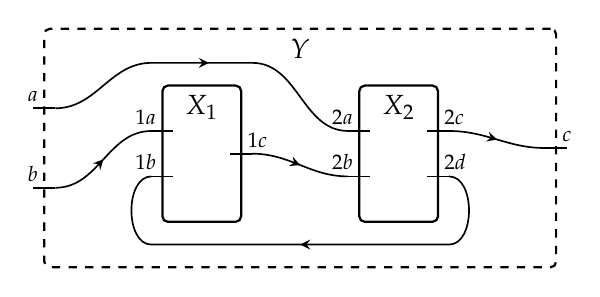
\begin{tikzpicture}[wiring diagram,baseline]
    \label{dia:string_diagram}
  \node[bb={2}{1}, bb name=$X_1$] (X1) {};
  \node[bb={2}{2}, right=of X1, bb name=$X_2$] (X2) {};
  \node[bb={2}{1}, dashed, fit={(X1) (X2) ($(X1.north)+(0,1.5)$) ($(X1.south)-(0,1)$)},
        bb name=$Y$] (Y) {};
  \draw[label]
    node[above left=of Y_in1]     {$a$}
    node[above left=of Y_in2]     {$b$}
    node[above right=of Y_out1]   {$c$}
    node[above left=of X1_in1]    {$1a$}
    node[above left=of X1_in2]    {$1b$}
    node[above right=of X1_out1]  {$1c$}
    node[above left=of X2_in1]    {$2a$}
    node[above left=of X2_in2]    {$2b$}
    node[above right=of X2_out1]  {$2c$}
    node[above right=of X2_out2]  {$2d$};
  \draw[ar] (Y_in2') to (X1_in1);
  \draw[ar] (X1_out1) to (X2_in2);
  \draw[ar] (X2_out1) to (Y_out1');
  \draw[ar] let \p1=(X1.north west), \p2=(X1.north east), \n1={\y1+\bby}, \n2=\bbportlen in
    (Y_in1') to (\x1-\n2,\n1) -- (\x2+\n2,\n1) to (X2_in1);
  \draw[ar] let \p1=(X2.south east), \p2=(X1.south west), \n1={\y1-\bby}, \n2=\bbportlen in
    (X2_out2) to[in=0] (\x1+\n2,\n1) -- (\x2-\n2,\n1) to[out=180] (X1_in2);
\end{tikzpicture}\end{equation}
represent compositions in a traced category $\cat{T}$. That is, new morphisms are constructed from
old by specifying which outputs will be fed back into which inputs. These are related to Penrose
diagrams in $\ncat{Vect}$ and the word \emph{traced} originates in this vector space
terminology.

The string diagrams of \cite{JoyalStreetVerity} typically do not explicitly include the outer box
$Y$. If we include it, as in (\ref{dia:string_diagram}), the resulting \emph{wiring diagram} can be
given a seemingly new interpretation: it represents a 1-dimensional cobordism between oriented
0-manifolds. Indeed, the objects in $\Cob$ are signed sets $X=\inp{X}\sqcup\outp{X}$, each of which
can be drawn as a box with input wires $\inp{X}$ entering on the left and output wires $\outp{X}$
exiting on the right.
\begin{equation*}
  \begin{tikzpicture}[node distance=0 and 0, baseline=(current bounding box.center)]
    \node (A1) {$-$};
    \node[below=-.1 of A1] (A2) {$-$};
    \node[below=-.1 of A2] (A3) {$-$};
    \node[below=-.1 of A3] (B1) {$+$};
    \node[below=-.1 of B1] (B2) {$+$};
  \end{tikzpicture}
  \hspace{4em}
  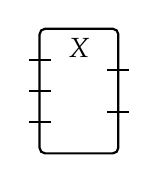
\begin{tikzpicture}[wiring diagram, bby=1.2ex, baseline=(current bounding box.center)]
    \node[bb={3}{2},bb name=$X$] {};
  \end{tikzpicture}
\end{equation*}
Moreover, the wiring diagram itself in which boxes $X_1,\ldots,X_n$ are wired together inside a
larger box $Y$ can be interpreted as an oriented cobordism from $X_1\sqcup\cdots\sqcup X_n$ to $Y$.
In fact, this is more appropriately interpreted as a morphism in the (colored) operad $\Cob$
underlying the symmetric monoidal category of oriented 1-cobordisms. The
following shows the two approaches to drawing a 2-ary morphism $X_1,X_2\to Y$ in $\LCob{\LabSet}$\todo{$\LCob{\LabSet}$ hasn't been introduced yet, move this lower?}:
\begin{equation*}
  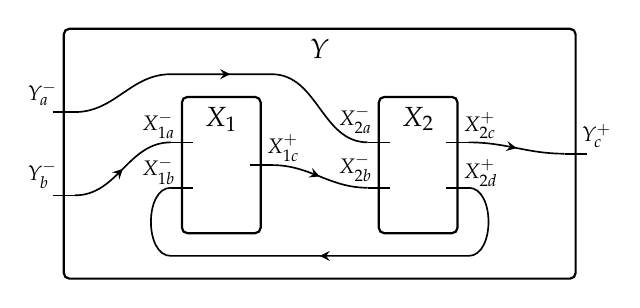
\begin{tikzpicture}[wiring diagram, baseline=(current bounding box.center)]
    \node[bb={2}{1}, bb name=$X_1$] (X1) {};
    \node[bb={2}{2}, right=of X1, bb name=$X_2$] (X2) {};
    \node[bb={2}{1}, fit={(X1) (X2) ($(X1.north)+(0,2)$) ($(X1.south)-(0,1)$)},bb name =$Y$] (Y) {};
    \draw[label]
      node[above left=of Y_in1]     {$\inp{Y}_a$}
      node[above left=of Y_in2]     {$\inp{Y}_b$}
      node[above right=of Y_out1]   {$\outp{Y}_c$}
      node[above left=1pt and -2pt of X1_in1]    {$\inp{X}_{1a}$}
      node[above left=1pt and -2pt of X1_in2]    {$\inp{X}_{1b}$}
      node[above right=1pt and -2pt of X1_out1]  {$\outp{X}_{1c}$}
      node[above left=3pt and -2pt of X2_in1]    {$\inp{X}_{2a}$}
      node[above left=2pt and -2pt of X2_in2]    {$\inp{X}_{2b}$}
      node[above right=1pt and -2pt of X2_out1]  {$\outp{X}_{2c}$}
      node[above right=0pt and -2pt of X2_out2]  {$\outp{X}_{2d}$};
    \draw[ar] (Y_in2') to (X1_in1);
    \draw[ar] (X1_out1) to (X2_in2);
    \draw[ar] (X2_out1) to (Y_out1');
    \draw[ar] let \p1=(X1.north west), \p2=(X1.north east), \n1={\y1+\bby}, \n2=\bbportlen in
      (Y_in1') to (\x1-\n2,\n1) -- (\x2+\n2,\n1) to (X2_in1);
    \draw[ar] let \p1=(X2.south east), \p2=(X1.south west), \n1={\y1-\bby}, \n2=\bbportlen in
      (X2_out2) to[in=0] (\x1+\n2,\n1) -- (\x2-\n2,\n1) to[out=180] (X1_in2);
  \end{tikzpicture}
  \qquad\quad
  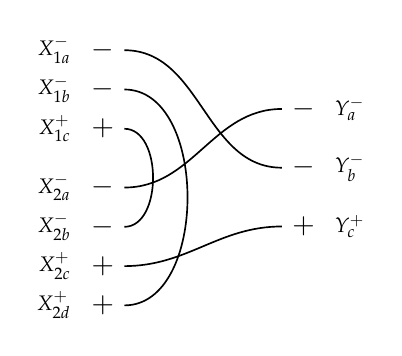
\begin{tikzpicture}[x=1cm,y=1ex,node distance=1 and 1,semithick,every label quotes/.style={font=\everymath\expandafter{\the\everymath\scriptstyle}},every to/.style={out=0,in=180},baseline=(current bounding box.center)]
    \node ["$\inp{X}_{1a}$" left] (X1a) {$-$};
    \node [below=0 of X1a, "$\inp{X}_{1b}$" left] (X1b) {$-$};
    \node [below=0 of X1b, "$\outp{X}_{1c}$" left] (X1c) {$+$};
    \node [below=1.5 of X1c, "$\inp{X}_{2a}$" left] (X2a) {$-$};
    \node [below=0 of X2a, "$\inp{X}_{2b}$" left] (X2b) {$-$};
    \node [below=0 of X2b, "$\outp{X}_{2c}$" left] (X2c) {$+$};
    \node [below=0 of X2c, "$\outp{X}_{2d}$" left] (X2d) {$+$};
    \node [below right=1.5 and 2 of X1a, "$\inp{Y}_a$" right] (Ya) {$-$};
    \node [below=1.5 of Ya, "$\inp{Y}_b$" right] (Yb) {$-$};
    \node [below=1.5 of Yb, "$\outp{Y}_c$" right] (Yc) {$+$};
    \draw (X1a) to (Yb);
    \draw (X1b) to[in=0] (X2d);
    \draw (X1c) to[in=0] (X2b);
    \draw (X2a) to (Ya);
    \draw (X2c) to (Yc);
  \end{tikzpicture}
\end{equation*}

There is actually a bit more data in a string (or wiring) diagram for a traced category $\cat{T}$
than in a cobordism. Namely, each input and output of a box must be labeled by an object of
$\cat{T}$ and the wires connecting boxes must respect the labels (e.g.\ in
(\ref{dia:string_diagram}) objects $1c$ and $2b$ must be equal). We will thus consider the operad
$\LCob{\LabSet}$ of oriented 1-dimensional cobordisms over a fixed set of labels $\LabSet$. We also
write $\LCob{\LabSet}$ to denote the corresponding symmetric monoidal category.

In the table below, we record these two interpretations of a string diagram. Note the ``degree
shift'' between the second and third columns.
\begin{center}
  \setlength{\tabcolsep}{10pt}
  \begin{tabular}{lll}
    \toprule
    \multicolumn{3}{c}{Interpretations of string diagrams} \\
    \midrule
    String diagram & Traced category $\cat{T}$ & $\LCob{\LabSet}$ \\
    \midrule
    Wire label set, $\LabSet$ & Objects, $\LabSet\coloneqq\Ob(\cat{T})$ & Label set, $\LabSet$ \\
    Boxes,
    e.g.~\tikz[wiring diagram,bb port sep=1,bby=2.4pt,bb min width=5.5pt,
          bb port length=2pt,bb rounded corners=1pt,baseline=(B.south)]
      {\node[bb={1}{2}] (B) {};}
    & Morphisms in $\cat{T}$& Objects (oriented 0-mfds over $\LabSet$) \\
    String diagrams & Compositions in $\cat{T}$& Morphisms (cobordisms over $\LabSet$) \\
    Nesting & Axioms of traced cats & Composition (of cobordisms) \\
    \bottomrule
  \end{tabular}
\end{center}

In the last row above, each of the seven axioms of traced categories is vacuous from the cobordism
perspective in the sense that both sides of the equation correspond to the same cobordism (up to
diffeomorphism). For example, the axiom of \emph{superposition} reads:
\[
  \Tr^U_{X,Y}\big[f\big]\otimes g=\Tr^U_{X\otimes W,Y\otimes Z}\big[f\otimes g\big]
\]
for every $f\colon U\otimes X\to U\otimes Y$ and $g\colon W\to Z$, or diagramatically:
\[\tikzset{bbx=.8cm,bb port sep=1.5}
  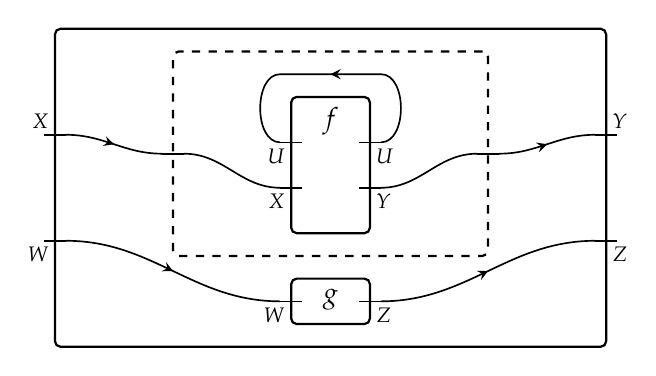
\begin{tikzpicture}[wiring diagram,baseline=(current bounding box.center)]
    \node[bb={2}{2}, bb name=$f$] (X1) {};
    \node[bb port sep=1,bb={1}{1}, below=2 of X1, bb name=$g$] (X2) {};
    \node[bb={1}{1}, fit={(X1) ($(X1.north)+(0,1)$)}, dashed] (Z) {};
    \node[bb={2}{2}, fit={(Z) (X2)}] (Y) {};
    \draw[ar] (Y_in1') to (Z_in1);
    \draw (Z_in1') to (X1_in2);
    \draw[ar] (Y_in2') to (X2_in1);
    \draw (X1_out2) to (Z_out1');
    \draw[ar] (Z_out1) to (Y_out1');
    \draw[ar] (X2_out1) to (Y_out2');
    \draw[ar] let \p1=(X1.north east), \p2=(X2.north west), \n1={\y1+\bby}, \n2=\bbportlen in
      (X1_out1) to[in=0] (\x1+\n2,\n1) -- (\x2-\n2,\n1) to[out=180] (X1_in1);
    \draw[label]
      node[above left=of Y_in1] {$X$}
      node[below left=of Y_in2] {$W$}
      node[above right=of Y_out1] {$Y$}
      node[below right=of Y_out2] {$Z$}
      node[below left=of X1_in1] {$U$}
      node[below left=of X1_in2] {$X$}
      node[below right=of X1_out2] {$Y$}
      node[below right=of X1_out1] {$U$}
      node[below left=of X2_in1] {$W$}
      node[below right=of X2_out1] {$Z$};
  \end{tikzpicture}
  \quad=\quad
  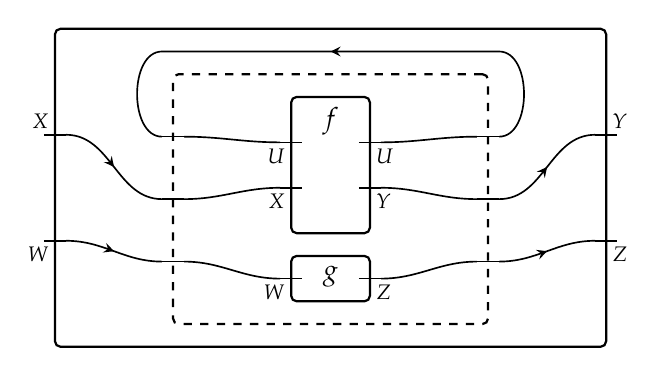
\begin{tikzpicture}[wiring diagram,baseline=(current bounding box.center)]
    \node[bb={2}{2}, bb name=$f$] (X1) {};
    \node[bb port sep=1,bb={1}{1}, below=of X1, bb name=$g$] (X2) {};
    \node[bb={3}{3}, fit={(X1) (X2)}, dashed] (Z) {};
    \node[bb={2}{2}, fit={(Z) ($(Z.north)+(0,1)$)}] (Y) {};
    \draw[ar] (Y_in1') to (Z_in2);
    \draw (Z_in2') to (X1_in2);
    \draw[ar] (Y_in2') to (Z_in3);
    \draw (Z_in3') to (X2_in1);
    \draw (X1_out2) to (Z_out2');
    \draw[ar] (Z_out2) to (Y_out1');
    \draw (X2_out1) to (Z_out3');
    \draw[ar] (Z_out3) to (Y_out2');
    \draw (Z_in1') to (X1_in1);
    \draw (X1_out1) to (Z_out1');
    \draw[ar] let \p1=(Z.north east), \p2=(Z.north west), \n1={\y1+\bby}, \n2=\bbportlen in
      (Z_out1) to[in=0] (\x1+\n2,\n1) -- (\x2-\n2,\n1) to[out=180] (Z_in1);
    \draw[label]
      node[above left=of Y_in1] {$X$}
      node[below left=of Y_in2] {$W$}
      node[above right=of Y_out1] {$Y$}
      node[below right=of Y_out2] {$Z$}
      node[below left=of X1_in1] {$U$}
      node[below left=of X1_in2] {$X$}
      node[below right=of X1_out2] {$Y$}
      node[below right=of X1_out1] {$U$}
      node[below left=of X2_in1] {$W$}
      node[below right=of X2_out1] {$Z$};
  \end{tikzpicture}
\]

To make precise the relationship between these interpretations of string diagrams, we fix the set
$\LabSet$ of labels. Let $\TrCat$ denote the 1-category of traced categories and traced strict
monoidal functors. Write $\TrCat_{\LabSet}$ for the subcategory consisting of those traced
categories $\cat{T}$ for which the monoid of objects is free on the set $\LabSet$, with
identity-on-objects functors $\cat{T}\to\cat{T}'$ between them.

\begin{named}{Theorem 0}
    \label{thm:traced_is_cob_alg}
  There is an equivalence of 1-categories
  \begin{equation}
      \label{eq:single_fiber_tr}
    \LCob{\LabSet}\alg\equiv\TrCat_{\LabSet},
  \end{equation}
  where, given any monoidal category $\cat{M}$, we denote by
  $\cat{M}\alg\coloneqq\ncat{Lax}(\cat{M},\Set)$ the category of lax functors $\cat{M}\to\Set$ and
  monoidal natural transformations.
\end{named}

To build intuition for this statement note that the same data are required, and the same conditions
are satisfied, whether one is specifying a lax functor $P\in\LCob{\LabSet}\alg$ or a traced category
$\cat{T}\in\TrCat_{\LabSet}$ with objects freely generated by the set $\LabSet$. First, for each box
$X=(\inp{X},\outp{X})$ that might appear in a string diagram, both $P\colon\LCob{\LabSet}\to\Set$
and $\cat{T}$ require a set, $P(X)$ and $\Hom_{\cat{T}}(\inp{X},\outp{X})$, respectively. Second,
for each string diagram, both $P$ and $\cat{T}$ require a function: an action on morphisms in the
case of $P$ and a formula for performing the required compositions, tensors, and traces in the case
of $\cat{T}$. The condition that $P$ is functorial corresponds to the fact that $\cat{T}$ satisfies
the axioms of traced categories.

We will briefly specify how to construct a lax functor $P$ from a traced category
$(\cat{T},\otimes,I,\Tr)$ whose objects are freely generated by $\LabSet$. In what follows, we abuse
notation slightly: given a relative set $\iota\colon Z\to\LabSet$ we will use the same symbol $Z$ to
denote the tensor $\bigotimes_{z\in Z}\iota(z)$ in $\cat{T}$. For an oriented 0-manifold
$X=\inp{X}\sqcup \outp{X}$ over $\LabSet$, put $P(X)\coloneqq\Hom_{\cat{T}}(\inp{X},\outp{X})$.
Given a cobordism $\Phi\colon X\to Y$, we need a function $P(\Phi)\colon P(X)\to P(Y)$. To specify
it, note that for any cobordism $\Phi$ there exist $A,B,C,D,E\in\Ob(\cat{T})$ such that
$\inp{X}\cong C\otimes A$, $\outp{X}\cong C\otimes B$, $\inp{Y}\cong A\otimes D$, $\outp{Y}\cong
B\otimes D$, and $E$ is the set of floating loops in $\Phi$; thus $\Phi$ is essentially equivalent
to the cobordism shown on the left side of (\ref{eq:cob_and_trace_pic}).
\begin{equation}
    \label{eq:cob_and_trace_pic}
  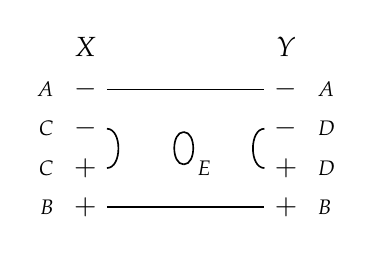
\begin{tikzpicture}[
      x=1cm, y=1ex, node distance=1 and 1, semithick,
      every label quotes/.style={font=\everymath\expandafter{\the\everymath\scriptstyle}},
      every to/.style={out=0,in=180},
      baseline=(current bounding box.center)
    ]
    \node ["$A$" left] (X1a) {$-$};
    \node [above=0.25 of X1a] {$X$};
    \node [below=0 of X1a, "$C$" left] (X1b) {$-$};
    \node [below=0 of X1b, "$C$" left] (X2a) {$+$};
    \node [below=0 of X2a, "$B$" left] (X2b) {$+$};
    \node [right=2 of X1a, "$A$" right] (Y1a) {$-$};
    \node [above=0.25 of Y1a] {$Y$};
    \node [below=0 of Y1a, "$D$" right] (Y1b) {$-$};
    \node [below=0 of Y1b, "$D$" right] (Y2a) {$+$};
    \node [below=0 of Y2a, "$B$" right] (Y2b) {$+$};
    \node [right=1.45 of X2a, "$E$" left] {};
    \draw (X1a) to (Y1a);
    \draw (X1b) to[in=0] (X2a);
    \draw (X2b) to (Y2b);
    \draw (Y1b) to[in=180,out=180] (Y2a);
    \draw ($(X1b)+(1.25,-2.75)$) to[in=0] ($(X1b)+(1.25,-0.25)$);
    \draw ($(X1b)+(1.25,-0.25)$) to[in=180,out=180] ($(X1b)+(1.25,-2.75)$);
  \end{tikzpicture}
  \qquad\qquad
  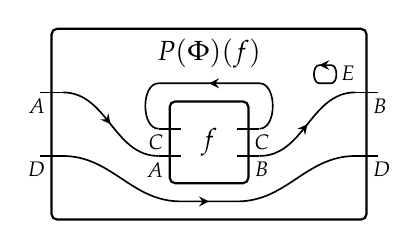
\begin{tikzpicture}[wiring diagram, bby=1.4ex, baseline=(current bounding box.center)]
    \node[bb port sep=1.5, bb={2}{2}] (domain) {$f$};
    \node[bb={2}{2}, fit={(domain) ($(domain.north)+(0,3)$) ($(domain.south)-(0,1)$)}, bb name=$P(\Phi)(f)$] (codomain) {};
    \draw[ar] (codomain_in1') to (domain_in2);
    \draw[ar] (domain_out2) to (codomain_out1');
    \draw[ar] let \p1=(domain.north east), \p2=(domain.north west), \n1={\y1+\bby}, \n2=\bbportlen in
      (domain_out1) to[in=0] (\x1+\n2,\n1) -- (\x2-\n2,\n1) to[out=180] (domain_in1);  %Trace on C
    \draw[ar] let \p1=(domain.south west), \p2=(domain.south east), \n1={\y1-\bby}, \n2=\bbportlen in
      (codomain_in2') to[in=180] (\x1+\n2,\n1) -- (\x2-\n2,\n1) to[out=0] (codomain_out2'); %Identity on D
    \draw[ar] let \p1=(domain.north east) in
      (\x1+.7*\bbx,\y1+\bby) to[in=0] (\x1+.7*\bbx,\y1+2*\bby) -- (\x1+.6*\bbx,\y1+2*\bby) to[out=180] (\x1+.6*\bbx,\y1+\bby) -- (\x1+.7*\bbx,\y1+\bby);%Loop
    \draw[label] let \p1=(domain.north east) in
      node[below left=of codomain_in1]     {$A$}
      node[below left=of codomain_in2]     {$D$}
      node[below right=of codomain_out1]    {$B$}
      node[below right=of codomain_out2]    {$D$}
      node[above left=.6 and 0 of codomain_out1']  {$E$}
      node[below left=of domain_in1]     {$C$}
      node[below left=of domain_in2]     {$A$}
      node[below right=of domain_out2]    {$B$}
      node[below right=of domain_out1]   {$C$};
  \end{tikzpicture}
\end{equation}
With the above notation, for $f\in P(X)$ we can follow the string diagram (right side of
(\ref{eq:cob_and_trace_pic})) and define
\begin{equation}
    \label{eq:cob algebra formula}
  P(\Phi)(f)\coloneqq\Tr_{A,B}^C[f]\otimes D\otimes\Tr^E_{I,I}[E],
\end{equation}
where we abuse notation and write $D$ and $E$ for the identity maps on these objects. One may easily
check, using each axiom of the trace \cite{JoyalStreetVerity} in an essential way, that
\eqref{eq:cob algebra formula} defines an algebra over $\LCob{\LabSet}$. We will not prove
\ref{thm:traced_is_cob_alg} directly as indicated here but to specify our proof strategy we must
introduce more notation.

\section{The main results}
  \label{sec:main_results}

The equivalence \eqref{eq:single_fiber_tr} has two significant conceptual drawbacks: the object set
of the traced category is fixed, and it is assumed to be freely generated by some set under tensor
products and functors are assumed strict; we refer to this latter condition using the term
\emph{objectwise-free}. Much of the work in this paper goes towards relaxing these two conditions.

To overcome the use of a fixed object set, we first explain what kind of object variance is
appropriate. There is an adjunction
\[
  \Adjoint{\Set}{\TrCat}{\FT}{\UT}
\]
inducing a monad $\TT$ on $\Set$, which is in fact isomorphic to the free monoid monad. Let
$\cat{T}$ and $\cat{T}'$ be objectwise-free traced categories where $\Ob(\cat{T})$ is the free
monoid on a set $\LabSet$ and $\Ob(\cat{T}')$ is the free monoid on a set $\LabSet'$. A strict
(traced) monoidal functor $F\colon \cat{T}\to \cat{T}'$ induces a homomorphism
$\Ob(F)\colon\Ob(\cat{T})\to\Ob(\cat{T}')$ between the free monoids, or equivalently a function $\Ob
F\colon\LabSet\to\TT(\LabSet')$ which can be identified with a morphism in the Kleisli category
$\Set_{\TT}$ of this monad.

The compact category $\LCob{\LabSet}$ clearly varies functorially in $\LabSet\in\Set$, but it is not
much harder to see that it is also functorial in $\LabSet\in\Set_{\TT}$.  This gives rise to a functor
\[
  (\LCob{\bullet})\colon\Set_{\TT}\to\CompCat
\]
to the category $\CompCat$ of compact categories and strict functors, sending $\LabSet$ to
$\LCob{\LabSet}$, the free compact category on $\LabSet$ (e.g.\ see \cite{KellyLaplaza,Abramsky2}).
We can compose this with $\Lax(-,\Set)$ to obtain a functor which we denote
\begin{equation}
    \label{eqn:cob/bullet}
  (\LCob{\bullet})\alg\colon\Set_{\TT}^{\mathrm{op}}\too\Cat.
\end{equation}
By applying the Grothendieck construction (denoted by $\int$ here) to (\ref{eqn:cob/bullet}), we
obtain a fibration for which the fiber over a set $\LabSet$ is equivalent (by
\ref{thm:traced_is_cob_alg}) to $\TrCat_{\LabSet}$. Let $\TrFrObCat\subset\TrCat$ denote the full
subcategory spanned by the objectwise-free traced categories.

\begin{named}{Theorem A}
    \label{thm:TheoremA_statement}
  There is an equivalence of 1-categories
  \begin{align*}
    &\int^{\LabSet\in\Set_{\TT}}(\LCob{\LabSet})\alg \to \TrFrObCat.
  \end{align*}
\end{named}

This result is proven in Section~\ref{sec:monoids_on_free} together with an analogous statement for
compact categories.

The fact that the traced categories appearing in \ref{thm:TheoremA_statement} are assumed
objectwise-free and the functors between them are strict is the second of two drawbacks mentioned
above. To address it, we prove that the 2-category of traced categories and strong functors is
biequivalent to that of objectwise-free traced categories and strict functors; see
Corollary~\ref{cor:object_frees}. This result seems to be well-known to experts but is difficult to
find in the literature.

In the course of proving \ref{thm:TheoremA_statement}, we will also establish generalizations
characterizing lax functors out of arbitrary compact categories, and in particular lax functors out
of $\Int(\cat{T})$ for an arbitrary traced category $\cat{T}$. In order to state this
characteization, we prove (Theorem~\ref{thm:orthogonal} and Proposition~\ref{prop:CompProf_exact})
that the well-known $(\bo,\ff)$ factorization system of $\Cat$ restricts to a factorization system
on $\TrCat$; more precisely the left class consists of bijective-on-objects functors and the right
class consists of fully faithful functors.

Write $\TrCat^{\bo}$ for the full subcategory of the arrow category $\TrCat^{\to}$ spanned by the
bijective-on-objects functors. The existence of the factorization system implies that the domain
functor
\[
  \dom\colon\TrCat^{\bo}\twoheadrightarrow\TrCat
\]
is a fibration. For a fixed traced category $\cat{T}$, the fiber
$\TrCat^{\bo}_{\cat{T}/}\coloneqq\dom^{-1}(\cat{T})$ is the category of strict monoidal,
bijective-on-objects functors from $\cat{T}$ to another traced category, with the evident
commutative triangles as morphisms. Note that we have an isomorphism
$\TrCat_{\LabSet}\iso\TrCat^{\bo}_{(\FT\LabSet)/}$.

Recall from~\cite{JoyalStreetVerity} that traced categories can be thought of as full subcategories
of compact categories: the Int construction applied to a traced category $\cat{T}$ builds the
smallest compact category $\Int(\cat{T})$ of which $\cat{T}$ is a monoidal subcategory. Generalizing
\eqref{eq:single_fiber_tr}, we can give a complete characterization of lax functors out of such
compact categories: for a fixed traced category $\cat{T}$ there is an equivalence of categories
\[
  \Lax(\Int(\cat{T}),\Set)\equiv\TrCat^{\bo}_{\cat{T}/}.
\]
In Section~\ref{sec:exactness_proofs} we show that these equivalences glue together to form an
equivalence of fibrations:

\begin{named}{Theorem B}
    \label{thm:TheoremB_statement}
  There is an equivalence of fibrations
  \begin{equation*}
    \begin{tikzcd}[column sep=-1em]
      \int\limits^{\mathclap{\cat{T}\in\TrCat}} \Lax(\Int(\cat{T}),\Set)
        \ar[rr,"\equiv"] \ar[dr,two heads]
      && \TrCat^{\bo} \ar[dl,two heads,"\dom" pos=.4] \\
      & \TrCat. &
    \end{tikzcd}
  \end{equation*}
\end{named}

Our main tool in proving this result will be the 2-categorical notion of \emph{(proarrow)
equipments}, which we recall in Section~\ref{chap:background_equipments}. We will introduce what
appears to be a new definition of \emph{monoidal profunctors}, and the equipment thereof, in
Section~\ref{chap:equipments_monoidal_profunctors}.

\section{Plan of the paper}

Section~\ref{sec:equipments} reviews the notion of an equipment (or framed bicategory
\cite{Shulman}), while Section~\ref{sec:monoids_bimods} recalls monoids and bimodules in an
equipment. Section~\ref{sec:exactness_boff} defines \emph{exact equipments}, which are central to
our proof strategy, and which we believe to be of independent interest. The material of this section
is original, though some of it appeared in the earlier unpublished \cite{Schultz2015}. In the short
Section~\ref{sec:internal_presheaves} we define (co)presheaves internal to an equipment, which will
allow us to reformulate our main theorems in terms of equipments.

In Section~\ref{sec:monoidal,compact,traced} we briefly review monoidal, traced, and compact
categories. We finally introduce various equipments of monoidal profunctors ($\dMonProf, \dTrProf$,
and $\dCompProf$) at the heart of the paper in Section~\ref{sec:monoidal_profunctors}. In
Section~\ref{sec:special_CompProf} we prove the special properties about $\dCompProf$ which are at
the core of our results. Indeed one might view the rest of the paper as a formal wrapper for the
results in that section. In Section~\ref{sec:exactness_proofs} we prove that the equipments of
interest are exact, and apply the theory developed in Section~\ref{chap:background_equipments} to
deduce \ref{thm:TheoremB}. In Section~\ref{sec:monoids_on_free} we deal with the objectwise-freeness
needed for \ref{thm:TheoremA}.

The appendix contains material that is not essential for establishing the main results of the paper. Its function is to prove the
biequivalence between the 2-category $\MMonCatStrong$ of monoidal categories with arbitrary object
set and strong functors, on the one hand, and the 2-category $\MMonFrObCat$ of monoidal categories
with free object set and strict functors. We do the same for traced and compact categories, all in
Corollary~\ref{cor:object_frees}.

\section*{Acknowledgments}

Thanks go to Steve Awodey and Ed Morehouse for suggesting we formally connect the operad-algebra
picture in \cite{RupelSpivak} to string diagrams in traced categories. We also thank Mike Shulman
for many useful conversations, and Tobias Fritz, Justin Hilburn, Dmitry Vagner, and Christina
Vasilakopoulou for helpful comments on drafts of this paper. Finally, we thank our referee for many
useful suggestions.

\chapter{Background on equipments}
  \label{chap:background_equipments}

This section introduces equipments, which we use to properly situate traced and compact categories.
This tool will eventually allow us to clarify the relationship between strict monoidal functors
between monoidal categories and lax monoidal functors to $\Set$.

\section{Equipments}
  \label{sec:equipments}

A double category is a 2-category-like structure involving horizontal and vertical arrows, as well
as 2-cells. An equipment (sometimes called a \emph{proarrow equipment} or \emph{framed bicategory})
is a double category satisfying a certain fibrancy condition. In this section, we will spell this
out and give two relevant examples. An excellent reference is Shulman's paper \cite{Shulman}; see
also \cite{Wood1} and \cite{Wood2}.

\begin{definition}
  A \emph{double category}%
  \footnote{
    We will use many flavors of category in this paper. To help distinguish, we denote named
    1-categories, monoidal categories, and operads with bold roman letters, e.g.\ $\ncat{Cob}$, and
    unnamed 1-categories with script, e.g.\ $\cat{C}$. For named 2-categories or bicategories we do
    almost the same, but change the font of the first letter to calligraphic, such as
    $\nncat{T}{rCat}$; for unnamed 2-categories we use (unbold) calligraphic, e.g.\ $\ccat{D}$.
    Finally, for double categories we make the first letter blackboard bold, whether named (e.g.,
    $\ndcat{P}{rof}$) or unnamed (e.g., $\dcat{D}$).
  }
  $\dcat{D}$ consists of the following data:
  \begin{itemize}
    \item A category $\dcat{D}_0$, which we refer to as the \emph{vertical category} of $\dcat{D}$.
      For any two objects $c,d\in\dcat{D}_0$, we will write $\dcat{D}_0(c,d)$ for the set of
      vertical arrows from $c$ to $d$. We refer to objects of $\dcat{D}_0$ as objects of $\dcat{D}$.
    \item A category $\dcat{D}_1$, equipped with two functors
      $\lframe,\rframe\colon\dcat{D}_1\to\dcat{D}_0$, called the \emph{left frame} and \emph{right
      frame} functors. Given an object $M\in\Ob(\dcat{D}_1)$ with $c=\lframe(M)$ and
      $c'=\rframe(M)$, we say that $M$ is a \emph{proarrow} (or \emph{horizontal arrow}) \emph{from
      $c$ to $c'$} and write $M\colon c\tickar c'$. A morphism $\phi\colon M\to N$ in $\dcat{D}_1$
      is called a 2-cell, and is drawn as follows, where $f=\lframe(\phi)$ and $f'=\rframe(\phi)$:
      \begin{equation} \begin{tikzcd}
          \label{eqn:2cell}
        c \ar[r,tick,"M" domA] \ar[d,"f"']
          & c'\ar[d,"f'"] \\
        d \ar[r,tick,"N"' codA]
          & d'
        \twocellA{\phi}
      \end{tikzcd} \end{equation}
    \item A \emph{unit} functor $\unit\colon\dcat{D}_0\to\dcat{D}_1$, which is a strict section of
      both $\lframe$ and $\rframe$, i.e.\ $\lframe\circ\unit=\id_{\dcat{D}_0}=\rframe\circ\unit$. We
      will often abuse notation by writing $c$ for the unit proarrow $\unit(c)\colon c\tickar c$,
      and similarly for vertical arrows.
    \item A functor $\odot\colon\dcat{D}_1\times_{\dcat{D}_0}\dcat{D}_1\to\dcat{D}_1$, called
      \emph{horizontal composition}, which is weakly associative and unital in the sense that there
      are coherent unitor and associator isomorphisms. See \cite{Shulman} for more details.
   \end{itemize}
  Given a double category $\dcat{D}$ there is a strict 2-category called the \emph{vertical
  2-category}, denoted $\VVer(\dcat{D})$, whose underlying 1-category is $\dcat{D}_0$ and whose
  2-morphisms $f\Rightarrow f'$ are defined to be 2-cells \eqref{eqn:2cell} where $M=\unit(c)$ and
  $N=\unit(d)$ are unit proarrows. There is also a \emph{horizontal bicategory}, denoted
  $\HHor(\dcat{D})$, whose objects and 1-cells are the objects and horizontal 1-cells of $\dcat{D}$,
  and whose 2-cells are the 2-cells of $\dcat{D}$ of the form \eqref{eqn:2cell} such that $f=\id_c$
  and $f'=\id_{c'}$.

  A \emph{strong double functor} $F\colon\dcat{C}\to\dcat{D}$ consists of functors
  $F_0\colon\dcat{C}_0\to\dcat{D}_0$ and $F_1\colon\dcat{C}_1\to\dcat{D}_1$ commuting with the
  frames $\lframe$,$\rframe$, and preserving the unit $\unit$ and horizontal composition $\odot$ up
  to coherent isomorphism.
\end{definition}

Recall that a \emph{fibration} of categories $p\colon\cat{E}\to\cat{B}$ is a functor with a lifting
property: for every $f\colon b'\to b$ in $\cat{B}$ and object $e\in\cat{E}$ with $p(e)=b$, there
exists $e'\to e$ over $f$ that is \emph{cartesian}, i.e.\ universal in an appropriate sense. We
denote fibrations of 1-categories using two-headed arrows $\onto$.

\begin{definition}
    \label{def:equipment}
  An \emph{equipment} is a double category $\dcat{D}$ in which the frame functor
  \[
    (\lframe,\rframe)\colon\dcat{D}_1\onto\dcat{D}_0\times\dcat{D}_0
  \]
  is a fibration. If $f\colon c\to d$ and $f'\colon c'\to d'$ are vertical morphisms and $N\colon
  d\tickar d'$ is a proarrow, a cartesian morphism $M\to N$ in $\dcat{D}_1$ over $(f,f')$ is a
  2-cell
  \[ \begin{tikzcd}
    c \ar[r,tick, "M" domA] \ar[d,"f"']
      & c'\ar[d,"f'"] \\
    d \ar[r,tick,"N"' codA]
      & d'
    \twocellalt{A}{\tn{cart}}
  \end{tikzcd} \]
  which we call a \emph{cartesian 2-cell}. We refer to $M$ as the \emph{restriction of $N$ along $f$
  and $f'$}, written $M=N(f',f)$.
\end{definition}

For any vertical morphism $f\colon c\to d$ in an equipment $\dcat{D}$, there are two canonical
proarrows $\comp{f}\colon c\tickar d$ and $\conj{f}\colon d\tickar c$, called respectively the
\emph{companion} and \emph{conjoint} of $f$, defined by restriction:
\begin{equation*}
  \begin{tikzcd}
    c \ar[r,tick,"\comp{f}" domA] \ar[d,"f"']
    & d \ar[d,equal] \\
    d \ar[r,tick,"\unit(d)"' codA] & d
    \twocellA{\tn{cart}}
  \end{tikzcd}
  \quad
  \begin{tikzcd}
    d \ar[r,tick,"\conj{f}" domA] \ar[d,equal]
    & c \ar[d,"f"] \\
    d \ar[r,tick,"\unit(d)"' codA] & d.
    \twocellA{\tn{cart}}
  \end{tikzcd}
\end{equation*}
In \cite{Shulman}, it is shown that all restrictions can be obtained by composing with companions
and conjoints. In particular, $N(f,g)\iso\comp{f}\odot N\odot\conj{g}$ for any proarrow $N$.
Moreover, $\comp{f}$ and $\conj{f}$ form an adjunction in $\HHor(\dcat{D})$; we write
$\eta_f\colon\conj{f}\odot\comp{f}\to\unit(d)$ and
$\epsilon_f\colon\unit(c)\to\comp{f}\odot\conj{f}$ for the unit and counit of this adjunction.

Recall that a pseudo-pullback of a cospan $A_1\To{f_1}A\From{f_2}A_2$ in a 2-category $\ccat{C}$ is a diagram
\begin{equation}
    \label{eqn:pseudopullback}
  \begin{tikzcd}[sep=small]
    X \ar[r,"g_1"] \ar[d,"g_2"'] \ar[rd,phantom,"\overset{\alpha}{\footnotesize\cong}"]
      & A_2 \ar[d,"f_2"] \\
    A_1 \ar[r,"f_1"']
      & A
  \end{tikzcd}
\end{equation}
where the tuple $(X,g_1,g_2,\alpha)$ is universal, up to equivalence, for data of that shape.
Although this definition makes sense for any 2-category $\ccat{C}$, we will use it only in the
special case described in the next paragraph.

Let $\ccat{C}=\CCat$.  Suppose $f_2$ is a fibration and that the square \eqref{eqn:pseudopullback}
strictly commutes, i.e.\ that $\alpha$ is the identity. It is a standard fact that a strict pullback
of a Grothendieck fibration along an arbitrary functor is a fibration and that the strict pullback
is also a pseudo-pullback. The upshot is that $g_2$ is a pseudo-pullback if and only if, for any
strict pullback $g_2'$ of $f_2$ along $f_1$, the induced map $g_2\to g_2'$ is an equivalence of
fibrations.

\begin{definition}
    \label{def:local_equivalence}
  By an \emph{equipment functor}, we simply mean a strong double functor between equipments. We
  refer to an equipment functor $F\colon\dcat{C}\to\dcat{D}$ as a \emph{local equivalence} if the
  following (strictly commuting) square is a pseudo-pullback of categories:
  \begin{equation} \begin{tikzcd}
      \label{eqn:local_equiv}
    \dcat{C}_1 \ar[r,"F_1"] \ar[d,two heads,"{(\lframe,\rframe)}"'] \ar[dr,phantom,"\lrcorner" very near start]
      & \dcat{D}_1 \ar[d,two heads,"{(\lframe,\rframe)}"] \\
    \dcat{C}_0\times\dcat{C}_0 \ar[r,"F_0\times F_0"']
      & \dcat{D}_0\times\dcat{D}_0.
  \end{tikzcd} \end{equation}
   If moreover $F_0\colon\dcat{C}_0\to\dcat{D}_0$ is fully faithful, we say that $F$ is a
   \emph{fully faithful local equivalence}.
\end{definition}

\begin{remark}
    \label{rem:strict_vs_pseudo_pullback}
  As discussed above, if the square \eqref{eqn:local_equiv} is a strict pullback, it will be a
  pseudo-pullback, and hence a local equivalence. Any local equivalence can be replaced by an
  equivalent strict pullback, which we define in
  Definition~\ref{def:induced_locally_equivalent_equipment}.

  Also note that the frame fibration for $\dcat{C}$ is equivalent to the functor
  $\dcat{C}_0\times\dcat{C}_0\to\CCat$, the 2-category of small categories, sending $(c,d)$ to
  $\HHor(\dcat{C})(c,d)$ and similarly for $\dcat{D}$. In this language, $F$ is a local equivalence
  if and only if the induced functors $\HHor(\dcat{C})(c,d)\to\HHor(\dcat{D})(F_0(c),F_0(d))$ are
  equivalences of categories for every pair of objects $(c,d)$. The square \eqref{eqn:local_equiv}
  is a strict pullback precisely when these are isomorphisms of categories.
\end{remark}

\begin{definition}
    \label{def:induced_locally_equivalent_equipment}
  Let $\dcat{D}$ be a double category and $F_0\colon\dcat{C}_0\to\dcat{D}_0$ be a functor. A strict
  pullback of the form \eqref{eqn:local_equiv} defines a double category $\dcat{C}$, which we denote
  \[
    \dcat{C}\coloneqq F_0^*(\dcat{D}).
  \]
  If $\dcat{D}$ is an equipment, $F_0^*(\dcat{D})$ will be as well since fibrations are stable under
  pullback. In this case we call $F_0^*(\dcat{D})$ the \emph{equipment induced by $F_0$}. By
  Remark~\ref{rem:strict_vs_pseudo_pullback}, the induced equipment functor
  $F_0^*(\dcat{D})\to\dcat{D}$ is a local equivalence.
\end{definition}

Our main tool in this paper will be equipments in which the horizontal arrows are (generalizations
of) profunctors, as in the following example.

\begin{example}
    \label{ex:profunctors}
  The equipment $\dProf$ is a double category whose vertical category $\dProf_0=\Cat$ is the
  category of small 1-categories and functors. Given categories $\cat{C},\cat{C}'\in\dProf_0$, a
  proarrow
  \[ \begin{tikzcd}
    \cat{C} \ar[r,tick,"M"] & \cat{C}'
  \end{tikzcd} \]
  in $\dProf_1$ is a profunctor, i.e.\ a functor $M\colon\op{\cat{C}}\times\cat{C}'\to\Set$. The
  left and right frame functors are given by $\lframe(M)=\cat{C}$ and $\rframe(M)=\cat{C}'$. A
  2-cell $\phi$ in $\dProf$, as to the left, denotes a natural transformation, as to the right, in
  \eqref{eqn:Prof2cells}:
  \begin{equation}
      \label{eqn:Prof2cells}
    \begin{tikzcd}
      \cat{C} \ar[r,tick,"M" domA] \ar[d,"F"']
        & \cat{C}'\ar[d,"F'"] \\
      \cat{D} \ar[r,tick,"N"' codA]
        & \cat{D}'
      \twocellA{\phi}
    \end{tikzcd}
    \hspace{.6in}
    \begin{tikzcd}[column sep=.8em, row sep=5ex]
      \op{\cat{C}}\times \cat{C}' \ar[dr,"M"'] \ar[rr,"\op{F}\times F'"]
        & \ar[d,phantom,"\overset{\phi}{\Rightarrow}" near start]
        & \op{\cat{D}}\times \cat{D}'\ar[dl,"N"] \\
      & \Set.
    \end{tikzcd}
  \end{equation}
  The unit functor $\unit\colon\Cat\to\dProf_1$ sends a category $\cat{C}$ to the hom profunctor
  $\Hom_{\cat{C}}\colon\op{\cat{C}}\times\cat{C}\to\Set$. Given two profunctors
  \[ \begin{tikzcd}
    \cat{C} \ar[r,tick,"M"] & \cat{D} \ar[r,tick,"N"] & \cat{E},
  \end{tikzcd} \]
  define the horizontal composition $M\odot N$ on objects $c\in\cat{C}$ and $e\in\cat{E}$ as the
  coequalizer of the diagram
  \begin{equation} \begin{tikzcd}
      \label{eqn:coendComp}
    \displaystyle\coprod_{d_1,d_2\in\cat{D}} M(c,d_1)\times\cat{D}(d_1,d_2)\times N(d_2,e)
      \ar[r,shift left] \ar[r,shift right]
    & \displaystyle\coprod_{d\in\cat{D}} M(c,d)\times N(d,e)
  \end{tikzcd} \end{equation}
  where the two maps are given by the right and left actions of $\cat{D}$ on $M$ and $N$
  respectively. Note that the coequalizer \eqref{eqn:coendComp} is in fact a reflexive coequalizer,
  using $\id_d\in\cat{D}(d,d)$. Given a profunctor $M\colon\cat{C}\tickar\cat{C'}$ there are
  canonical isomorphisms $\Hom_{\cat{C}}\odot M \iso M \iso M\odot\Hom_{\cat{D}}$ which can be
  viewed as giving an action of $\Hom_{\cat{C}}$ and of $\Hom_{\cat{D}}$ on $M$, from the left and
  right respectively.

  At this point we have given $\dProf$ the structure of a double category. To see that $\dProf$ is
  an equipment, note that from a pair of functors $F\colon\cat{C}\to\cat{D}$,
  $F'\colon\cat{C}'\to\cat{D}'$ and a profunctor $N\colon \cat{D}\tickar\cat{D}'$ we may form the
  composite
  \[\begin{tikzcd}
    \op{\cat{C}}\times\cat{C}' \ar[r,"\op{F}\times F'"]
      &[1.5em] \op{\cat{D}}\times\cat{D}' \ar[r,"N"]
      & \Set,
  \end{tikzcd}\]
  denoted $N(F',F)\colon\cat{C}\tickar\cat{C}'$, such that
  \begin{equation}
      \label{eq:cartesian profunctor morphism}
    \begin{tikzcd}
      \cat{C} \ar[r,tick,"{N(F',F)}" domA] \ar[d,"F"']
        & \cat{C}'\ar[d,"F'"] \\
      \cat{D} \ar[r,tick,"N"' codA]
        & \cat{D}'
      \twocellA{\phi}
    \end{tikzcd}
  \end{equation}
  is a cartesian 2-cell. A simple Yoneda lemma argument yields $\VVer(\dProf)\equiv\CCat$.
\end{example}

\begin{remark}
    \label{rmk:profunctor_as_bimodule}
  There is a strong analogy relating profunctors between categories with bimodules between rings.
  Besides being a useful source of intuition, we can also exploit this analogy to provide a
  convenient notation for working with profunctors.

  If $M\colon\op{\cat{C}}\times\cat{D}\to\Set$ is a profunctor, then for any element $m\in M(c,d)$
  and morphisms $f\colon c'\to c$ and $g\colon d\to d'$, we can write $g\cdot m\in M(c,d')$ and
  $m\cdot f\in M(c',d)$ for the elements $M(\id,g)(m)$ and $M(f,\id)(m)$ respectively. Thus we think
  of the functoriality of $M$ as providing left and right actions of $\cat{D}$ and $\cat{C}$ on the
  elements of $M$. The equations $(g\cdot m)\cdot f = g\cdot (m\cdot f)$, $g'\cdot(g\cdot
  m)=(g'\circ g)\cdot m$, and $(m\cdot f)\cdot f'=m\cdot(f\circ f')$ clearly hold whenever they
  make sense.

  The coequalizer \eqref{eqn:coendComp} can be easily expressed in this notation: the elements of
  $(M\odot N)(c,e)$ are pairs $m\otimes n$ of elements $m\in M(c,d)$ and $n\in N(d,e)$ for some
  $d\in\cat{D}$ modulo the relation $(m\cdot f)\otimes n = m\otimes(f\cdot n)$, whenever this makes
  sense.

  Finally, a 2-cell $\phi$ of the form \eqref{eqn:Prof2cells} is function sending elements $m\in
  M(c,c')$ to elements $\phi(m)\in N(Fc,F'c')$ such that the equation $\phi(f\cdot m\cdot
  g)=F(f)\cdot\phi(m)\cdot F'(g)$ holds whenever it makes sense.
\end{remark}

\section{Monoids and bimodules}
  \label{sec:monoids_bimods}

Our eventual proofs of \ref{thm:TheoremA}~and~\ref{thm:TheoremB} will revolve around a careful
understanding of internal monoids in an equipment $\dcat{D}$. In particular,
following~\cite{Schultz2015}, the exactness of an equipment and the resulting $(\bo,\ff)$
factorization system, both given in Section~\ref{sec:exactness_boff}, are built on notions related
to monoids in $\dcat{D}$.

\begin{definition}
    \label{def:monoids}
  Denote by $\Mon(\dcat{D})$ the category of monoids in $\dcat{D}$. More precisely, the objects are
  \emph{monoids}: 4-tuples $(c,M,i_M,m_M)$ consisting of an object $c$ of $\dcat{D}$ and a proarrow
  $M\colon c\tickar c$ together with unit and multiplication cells
  \begin{equation}
      \label{eqn:unit_and_mult}
    \begin{tikzcd}
      c \ar[r,tick,"c" domA] \ar[d,equal]
        & c \ar[d,equal] \\
      c \ar[r,tick,"M"' codA] & c
      \twocellA{i_M}
    \end{tikzcd}
    \qquad
    \begin{tikzcd}
      c \ar[r,tick,"M"] \ar[d,equal]
        & |[alias=domA]| c \ar[r,tick,"M"]
        & c \ar[d,equal] \\
      c \ar[rr,tick,"M"' codA]
        && c
      \twocellA{m_M}
    \end{tikzcd}
  \end{equation}
  satisfying the evident unit and associativity axioms. The morphisms are \emph{monoid
  homomorphisms}: pairs $(f,\vec{f}\mspace{2mu})$ consisting of a vertical arrow $f\colon c\to d$ in
  $\dcat{D}$ and a cell
  \[ \begin{tikzcd}
    c \ar[r,tick,"M" domA] \ar[d,"f"']
      & c \ar[d,"f"] \\
    d \ar[r,tick,"N"' codA]
      & d
    \twocellA{\vec{f}}
  \end{tikzcd} \]
  which respects the unit and multiplication cells of $M$ and $N$.
\end{definition}

There is an evident forgetful functor $\MOb\colon\Mon(\dcat{D})\to\dcat{D}_0$ sending a monoid
$M\colon c\tickar c$ to its underlying object $|M|\coloneqq c$. The following result can also be
found in \cite{FioreGambinoKock}.

\begin{lemma}
    \label{lemma:Mon_und_fib}
  Let $\dcat{D}$ be an equipment. The forgetful functor $\MOb\colon\Mon(\dcat{D})\to\dcat{D}_0$ is a
  fibration and there is a morphism of fibrations
  \[ \begin{tikzcd}[column sep=tiny]
    \Mon(\dcat{D}) \ar[d,two heads,"\MOb"'] \ar[r]
      & \dcat{D}_1 \ar[d,two heads,"{(\lframe,\rframe)}"] \\
    \dcat{D}_0 \ar[r,"\Delta"']&\dcat{D}_0\times\dcat{D}_0.
  \end{tikzcd} \]
\end{lemma}
\begin{proof}
  Let $f\colon c\to d$ be a vertical morphism of $\dcat{D}$ and $N\colon d\tickar d$ a monoid in
  $\dcat{D}$. Since the 2-cell defining the restriction of $N$ along $f$ is cartesian, there is an
  induced monoid structure on $N(f,f)$ which in particular makes this cartesian 2-cell a monoid
  homomorphism. The result follows.
\end{proof}

\begin{lemma}
    \label{lem:Mon_pullback}
  For a local equivalence $F\colon\dcat{C}\to\dcat{D}$, the induced square
  \[ \begin{tikzcd}
    \Mon(\dcat{C}) \ar[r,"\Mon(F)"] \ar[d,two heads,"\MOb"'] \ar[dr,phantom,"\lrcorner" very near start]
      & \Mon(\dcat{D}) \ar[d,two heads,"\MOb"] \\
    \dcat{C}_0 \ar[r,"F_0"']
      & \dcat{D}_0
  \end{tikzcd} \]
  is a pseudo-pullback of categories.
\end{lemma}
\begin{proof}
  By Remark~\ref{rem:strict_vs_pseudo_pullback}, we may assume that the pullback in
  Definition~\ref{def:local_equivalence} realizing $F\colon\dcat{C}\to\dcat{D}$ as a local
  equivalence is strict. It is then straightforward to check directly that the above square is again
  a strict pullback and hence a pseudo-pullback.
\end{proof}

In all our cases of interest, $\Mon(\dcat{C})$ will be the vertical part of an equipment. The
following is a standard construction; see \cite{Shulman}

\begin{definition}
    \label{def:monoids_and_modules}
  Let $\dcat{D}$ be an equipment with local coequalizers, i.e.\ such that each category
  $\HHor(\dcat{D})(c,d)$ has coequalizers and $\odot$ preserves coequalizers in each variable. The
  equipment $\dMod(\dcat{D})$ of \emph{monoids and bimodules} is defined as follows:
  \begin{itemize}
    \item The vertical category $\dMod(\dcat{D})_0$ is the category $\Mon(\dcat{D})$ of monoids in
      $\dcat{D}$.
    \item The proarrows $B\colon M\tickar N$ are \emph{bimodules}: triples $(B,l_B,r_B)$
      consisting of a proarrow $B\colon c\tickar d$ in $\dcat{D}$ and cells
      \begin{equation*}
        \begin{tikzcd}
          c \ar[r,tick,"M"] \ar[d,equal]
            & |[alias=domA]| c \ar[r,tick,"B"]
            & d \ar[d,equal] \\
          c \ar[rr,tick,"B"' codA]
            && d
          \twocellA{l_B}
        \end{tikzcd}
        \qquad
        \begin{tikzcd}
          c \ar[r,tick,"B"] \ar[d,equal]
            & |[alias=domA]| d \ar[r,tick,"N"]
            & d \ar[d,equal] \\
          c \ar[rr,tick,"B"' codA]
          && d
          \twocellA{r_B}
        \end{tikzcd}
      \end{equation*}
      satisfying evident monoid action axioms.
    \item The horizontal composition $B_1\otimes_{M'} B_2$ of bimodules $B_1\colon M\tickar M'$ and
      $B_2\colon M'\tickar M''$ is given by the coequalizer in $\HHor(\dcat{D})(M,M'')$
      \[
        B_1\odot M'\odot B_2 \rightrightarrows B_1\odot B_2 \to B_1\otimes_{M'} B_2
      \]
      together with the evident left $M$ and right $M''$ actions.
    \item The 2-cells are \emph{bimodule homomorphisms}: cells in $\dcat{D}$
      \[ \begin{tikzcd}
        c \ar[r,tick,"A"] \ar[d,"f"' domA]
          & c' \ar[d,"f'" codA] \\
        d \ar[r,tick,"B"']
          & d'
        \twocellA{\phi}
      \end{tikzcd} \]
      which are compatible with the left and right actions of the bimodules.
  \end{itemize}
  We will write $\Bimod{M}{N}$ to denote the 1-category of $(M,N)$-bimodules and bimodule morphisms.
\end{definition}

The forgetful functor $\MOb\colon\Mon(\dcat{D})\to\dcat{D}_0$ extends to a forgetful equipment
functor $\MOb\colon\dMod(\dcat{D})\to\dcat{D}$. There is also a local equivalence
$U\colon\dcat{D}\to\dMod(\dcat{D})$ sending $c$ to the unit $c\tickar c$ with the trivial monoid
structure. If $F\colon\dcat{C}\to\dcat{D}$ is an equipment functor, then there is an evident
equipment functor $\dMod(F)\colon\dMod(\dcat{C})\to\dMod(\dcat{D})$. In fact, we have the following
which is immediate from the definitions.

\begin{lemma}
    \label{lemma:FFLE_Mod}
  For a local equivalence $F\colon\dcat{C}\to\dcat{D}$ the induced functor
  $\dMod(F)\colon\dMod(\dcat{C})\to\dMod(\dcat{D})$ is a local equivalence. If $F$ is a fully
  faithful local equivalence, then so is $\dMod(F)$.
\end{lemma}

\section{Exact equipments and $\bo$, $\ff$ factorization}
  \label{sec:exactness_boff}

\todo[inline]{Patrick: introduce this section.}
\begin{definition}
    \label{def:embedding}
  Let $M\colon c\tickar c$ be a monoid in an equipment $\dcat{D}$. An \emph{embedding} of $M$ into
  an object $x\in\dcat{D}_0$ is a monoid homomorphism $(f,\vec{f}\mspace{2mu})$ from $M$ to the
  trivial monoid on $x$:
  \[ \begin{tikzcd}
    c \ar[r,tick,"M" domA] \ar[d,"f"']
      & c \ar[d,"f"] \\
    x \ar[r,tick,"x"' codA]
      & x.
    \twocellA{\vec{f}}
  \end{tikzcd} \]
  We will sometimes write an embedding as $(f,\vec{f}\mspace{2mu})\colon(c,M)\to x$, or even just
  $f\colon M\to x$ when clear from context. We will write $\Emb(M,x)$ for the set of embeddings from
  $M$ to $x$. This defines a functor $\Emb\colon\op{\Mon(\dcat{D})}\times\dcat{D}_0\to\Set$.
\end{definition}

\begin{lemma}
    \label{lemma:embed_for_LE}
  Suppose that $F\colon\dcat{C}\to\dcat{D}$ is a local equivalence induced by
  $F_0\colon\dcat{C}_0\to\dcat{D}_0$. Suppose $M\in\Mon(\dcat{C})$ is a monoid and $x\in\dcat{C}_0$
  is an object. For $N=\Mon(F)(M)$ and $y=F_0(x)$ we have a pullback square in $\Set$, natural in
  $M$ and $x$:
  \[ \begin{tikzcd}
    \Emb_{\dcat{C}}(M,x)\ar[r]\ar[d]\ar[rd,phantom,"\lrcorner" very near start]
      & \Emb_{\dcat{D}}(N,y)\ar[d] \\
    \dcat{C}_0(|M|,x)\ar[r]
      & \dcat{D}_0(|N|,y).
  \end{tikzcd} \]
\end{lemma}

\begin{definition}
  Let $M\colon c\tickar c$ be a monoid in an equipment $\dcat{D}$. The \emph{collapse} of $M$ is
  defined to be a universal embedding of $M$. That is, the collapse of $M$ is an object
  $\Col{M}\in\dcat{D}_0$ together with an embedding
  \[ \begin{tikzcd}
    c \ar[r,tick,"M" domA] \ar[d,"i_M"']
      & c \ar[d,"i_M"] \\
    \Col{M} \ar[r,tick,"\Col{M}"' codA]
      & \Col{M}
    \twocellA{\vec{\imath}_M}
  \end{tikzcd} \]
  such that any other embedding of $M$ factors uniquely through $\vec{\imath}_M$:
  \begin{equation*}
    \begin{tikzcd}
      c \ar[r,tick,"M" domA] \ar[d,"f"']
        & c \ar[d,"f"] \\
      x \ar[r,tick,"x"']
        & x
      \twocellA{\vec{f}}
    \end{tikzcd}
    \quad = \quad
    \begin{tikzcd}
      c \ar[r,tick,"M" domA] \ar[d,"i_M"']
        & c \ar[d,"i_M"] \\
      \Col{M} \ar[r,tick,"\Col{M}"' {domB,codA}] \ar[d,"\tilde{f}"']
        & \Col{M} \ar[d,"\tilde{f}"] \\
      x \ar[r,tick,"x"' codB]
        & x.
      \twocellA{\vec{\imath}_M}
      \twocellB[pos=.6]{\id_{\tilde{f}}}
    \end{tikzcd}
  \end{equation*}
  In other words, $\Col{M}$ represents the functor $\Emb(M,\textrm{--})\colon\dcat{D}_0\to\Set$.
\end{definition}

\begin{remark}
    \label{rem:canonical_actions}
  For any monoid $M\colon c\tickar c$, the companion $\comp{i}_M\colon c\tickar \Col{M}$ (resp.\ the
  conjoint $\conj{i}_M\colon \Col{M}\tickar c$) of the embedding $i_M\colon c\to\Col{M}$ has the
  structure of a left (resp.\ right) $M$-module. Indeed, these are given by rewriting the collapse
  2-cell $\vec{\imath}_M$ as follows:\todo{I don't understand how to construct these diagrams.  It
  seems to me that we should consider the horizontal composition of $\vec{\imath}_M$ with the
  cartesian two-cell defining $\comp{i}_M$ to get a two-cell into $\Col{M}$, which then factors
  through $\comp{i}_M$ using the cartesian property.}
  \[
    \begin{tikzcd}
      c \ar[r,tick,"M"] \ar[d,equal]
        & |[alias=domA]| c \ar[r,tick,"\comp{i}_M"]
        & \Col{M} \ar[d,equal] \\
      c \ar[r,tick,"\comp{i}_M"']
        & |[alias=codA]| \Col{M} \ar[r,tick,"\Col{M}"']
        & \Col{M}
      \twocellA{}
    \end{tikzcd}
    \qquad\qquad
    \begin{tikzcd}
      \Col{M} \ar[r,tick,"\conj{i}_M"] \ar[d,equal]
        & |[alias=domA]| c \ar[r,tick,"M"]
        & c \ar[d,equal] \\
      \Col{M} \ar[r,tick,"\Col{M}"']
        & |[alias=codA]| \Col{M} \ar[r,tick,"\conj{i}_M"']
        & c
      \twocellA{}
    \end{tikzcd}
  \]
\end{remark}

\begin{lemma}
  Let $M\colon c\tickar c$ and $N\colon d\tickar d$ be monoids in an equipment $\dcat{D}$ and assume
  they admit collapses $\Col{M}$ and $\Col{N}$, respectively. Then restriction induces a functor
  \[
    \HHor(\dcat{D})(\Col{M},\Col{N})\to\Bimod{M}{N}.
  \]
\end{lemma}
\begin{proof}
  For a proarrow $X\colon\Col{M}\tickar\Col{N}$ of $\dcat{D}$, define $\tilde X\colon c\tickar d$ by
  the cartesian 2-cell
  \begin{equation}
      \label{eq:bimodule}
    \begin{tikzcd}
      c \ar[r,tick, "\tilde X" domA] \ar[d,"i_M"']
        & d\ar[d,"i_N"] \\
      \Col{M} \ar[r,tick,"X"' codA]
        & \Col{N}.
      \twocellA{\tn{cart}}
    \end{tikzcd}
  \end{equation}
  Then a 2-cell $X\Rightarrow Y$ immediately lifts to a 2-cell $\tilde X\Rightarrow \tilde Y$. Since
  \eqref{eq:bimodule} is cartesian, we obtain an equality
  \[ \begin{tikzcd}
    c \ar[r,tick,"M" domA] \ar[d,"i_M"']
      & c \ar[r,tick, "\tilde X" domB] \ar[d,"i_M"']
      & d\ar[d,"i_N"] \\
    \Col{M} \ar[r,tick,"\Col{M}"' codA] \ar[d,equal]
      & |[alias=domC]| \Col{M} \ar[r,tick,"X"' codB]
      & \Col{N} \ar[d,equal] \\
    \Col{M} \ar[rr,tick,"X"' codC]
      && \Col{N}
    \twocellA{\vec{\imath}_M}
    \twocellB{\tn{cart}}
    \twocelliso{C}{}
  \end{tikzcd}
  \quad = \quad
  \begin{tikzcd}
    c \ar[r,tick,"M"] \ar[d,equal]
      & |[alias=domA]| c \ar[r,tick,"\tilde X"]
      & d \ar[d,equal] \\
    c \ar[rr,tick,"\tilde X"' {codA,domB}] \ar[d,"i_M"']
      && d \ar[d,"i_N"]\\
    \Col{M} \ar[rr,tick,"X"' codB]
      && \Col{N}
    \twocellA{l_{\tilde X}}
    \twocellB{\tn{cart}}
  \end{tikzcd}\]
  giving the action of $M$ on $\tilde X$. The action $r_{\tilde X}$ of $N$ on $\tilde X$ is obtained
  similarly, and one easily checks the axioms making $\tilde X$ an $(M,N)$-bimodule.
\end{proof}

\begin{definition}\cite[Proposition 5.4]{Schultz2015}
    \label{def:exact_equipment}
  An equipment $\dcat{D}$ is \emph{exact} if the following hold:
  \begin{enumerate}
    \item every monoid $M\colon c\tickar c$ has a collapse $\Col{M}$ with $\vec{\imath}_M$
      cartesian;
    \item for every pair of monoids $M$ and $N$ the restriction functor
    \begin{equation}
        \label{eqn:exact_Hor_Bimod}
      \HHor(\dcat{D})(\Col{M},\Col{N})\To{\raisebox{-1ex}{$\equiv$}}\Bimod{M}{N}
    \end{equation}
    is an equivalence of categories.
  \end{enumerate}
\end{definition}

\begin{remark}
    \label{rmk:exact_equiv_fibrations}
  The restriction functor \eqref{eqn:exact_Hor_Bimod} is clearly natural, giving a natural
  equivalence between pseudo-functors $\op{\Mon(\dcat{D})}\times\op{\Mon(\dcat{D})}\to\CCat$, or
  equivalently an equivalence of fibrations the inverse of which gives rise to a strictly-commuting
  pseudo-pullback square
  \begin{equation*}
    \begin{tikzcd}
      \dMod(\dcat{D})_1 \ar[d,two heads] \ar[r]
      & \dcat{D}_1 \ar[d,two heads] \\
      \Mon(\dcat{D})\times\Mon(\dcat{D}) \ar[r,"\Col{\textrm{--}}\times\Col{\textrm{--}}"']
      & \dcat{D}_0\times\dcat{D}_0.
    \end{tikzcd}
  \end{equation*}
  We will show in Proposition~\ref{prop:collapse_local_equivalence} that this preserves horizontal
  composition, defining a double functor, and hence a local equivalence.
\end{remark}

\begin{example}
    \label{ex:exact_span_prof}
  It was proven in \cite[Proposition~5.2]{Schultz2015} that for any equipment $\dcat{D}$, its
  equipment $\dMod(\dcat{D})$ of monoids and bimodules is exact. Thus $\dProf$ is exact, since there
  is an equivalence $\dProf\cong\dMod(\dSpan)$, where $\dSpan$ is the equipment of spans in $\Set$;
  see \cite{Shulman}.
\end{example}

Exact equipments arising in practice almost always have local coequalizers, and in this case it is
possible to simplify the definition, as we show in Proposition~\ref{prop:exact_coeqs}. Recall from
Remark~\ref{rem:canonical_actions} the natural $M$-module structures on the companion
$\comp{i}_M\colon c\tickar \Col{M}$ and conjoint $\conj{i}_M\colon \Col{M}\tickar c$ of the collapse
embedding $i_M\colon c\to\Col{M}$. Recall also the notation $\unit(a)\colon a\tickar a$ for the unit
map on an object $a$.

\begin{proposition}
    \label{prop:exact_coeqs}
  Suppose $\dcat{D}$ is an equipment with local coequalizers which satisfies Condition 1 of
  Definition~\ref{def:exact_equipment}. Then $\dcat{D}$ satisfies Condition 2 if and only if for
  every monoid $M\colon c\tickar c$, the following diagram is a coequalizer in
  $\HHor(\dcat{D})(\Col{M},\Col{M})$:
  \begin{equation}
      \label{eqn:exact_coeq}
    \begin{tikzcd}
      \conj{i}_M\odot\comp{i}_M\odot\conj{i}_M\odot\comp{i}_M
        \ar[r,shift left,"\epsilon_{i_M}\odot\conj{i}_M\odot\comp{i}_M"]
        \ar[r,shift right,"\conj{i}_M\odot\comp{i}_M\odot\epsilon_{i_M}"']
      &[3.5em] \conj{i}_M\odot\comp{i}_M
        \ar[r,"\epsilon_{i_M}"]
      & \unit\Col{M}
    \end{tikzcd}
  \end{equation}
  or, equivalently, $\conj{i}_M\otimes_M\comp{i}_M\iso\unit\Col{M}$.
\end{proposition}
\begin{proof}
  By Condition~1 of Definition~\ref{def:exact_equipment}, we have $M\iso\comp{i}_M\odot\conj{i}_M$,
  so the final equivalence is just the definition of horizontal composition in $\dMod(\dcat{D})$;
  see Definition~\ref{def:monoids_and_modules} and Remark~\ref{rem:canonical_actions}. Below we will
  use the fact that, by definition of $\dcat{D}$ having local coequalizers, $\odot$ preserves
  coequalizers in each variable, and that $\otimes$ is defined as a coequalizer. Finally, note that
  the restriction functor \eqref{eqn:exact_Hor_Bimod} is isomorphic to the functor
  $X\mapsto\comp{i}_M\odot X\odot\conj{i}_N$, with the left and right actions given by the left
  action of $M$ on $\comp{i}_M$ and right action of $N$ on $\conj{i}_N$.

  Assuming $\conj{i}_M\otimes_M\comp{i}_M\iso\unit\Col{M}$, we can construct an inverse to this
  restriction functor, sending an $(M,N)$-bimodule $B$ to $\conj{i}_M\otimes_M
  B\otimes_N\comp{i}_N$. It is easy to check that this gives an equivalence of categories:
  \begin{align*}
    \conj{i}_M\otimes_M (\comp{i}_M\odot X\odot\conj{i}_N)\otimes_N\comp{i}_N
      &\iso (\conj{i}_M\otimes_M\comp{i}_M)\odot X\odot (\conj{i}_N\otimes_N\comp{i}_N) \\
      &\iso \unit\Col{M}\odot X\odot \unit\Col{N} \\
      &\iso X \\
    \intertext{and}
    \comp{i}_M\odot (\conj{i}_M\otimes_M B\otimes_N\comp{i}_N)\odot \conj{i}_N
      &\iso (\comp{i}_M\odot\conj{i}_M)\otimes_M B\otimes_N (\comp{i}_N\odot\conj{i}_N) \\
      &\iso M\otimes_M B\otimes_N N \\
      &\iso B.
  \end{align*}

  Conversely, assuming the functor \eqref{eqn:exact_Hor_Bimod} is an equivalence of categories, then
  we can prove that $\conj{i}_M\otimes_M\comp{i}_M\iso\unit\Col{M}$ is an isomorphism by first
  applying the restriction functor:
  \begin{align*}
    \comp{i}_M\odot(\conj{i}_M\otimes_M\comp{i}_M)\odot\conj{i}_M
      &\iso (\comp{i}_M\odot\conj{i}_M)\otimes_M(\comp{i}_M\odot\conj{i}_M) \\
      &\iso M\otimes_M M \\
      &\iso M \\
      &\iso \comp{i}_M\odot\conj{i}_M \\
      &\iso \comp{i}_M\odot\unit\Col{M}\odot\conj{i}_M. \qedhere
  \end{align*}
\end{proof}

\begin{example}
    \label{ex:monoid_in_Prof}
  While the exactness of $\dProf$ follows from formal reasons, as we saw in
  Example~\ref{ex:exact_span_prof}, it will be helpful to understand collapse in $\dProf$
  concretely.

  Consider a monoid $M\colon \cat{C}\tickar \cat{C}$ in $\dProf$. The unit is a profunctor morphism
  $i\colon\Hom_{\cat{C}}\to M$. So for any $f\colon c\to d$ in $\cat{C}$ there is an element
  $i(f)\in M(c,d)$, such that
  \begin{equation}
      \label{eq:Prof_monoid_unit}
    g\cdot i(f)\cdot h = i(g\circ f\circ h)
  \end{equation}
  whenever this makes sense.

  The multiplication $M\odot M\to M$ is an operation assigning to any elements $m_1\in M(c,d)$ and
  $m_2\in M(d,e)$ an element $m_2\bullet m_1\in M(c,e)$, which is associative and satisfies the
  following equations whenever they make sense:
  \begin{gather}
    (f\cdot m_2)\bullet(m_1\cdot h) = f\cdot(m_2\bullet m_1)\cdot h
      \label{eq:Prof_monoid_A}
    \\ (m_3\cdot g)\bullet m_1 = m_3\bullet(g\cdot m_1)
      \label{eq:Prof_monoid_B}
    \\ m\bullet i(f) = m\cdot f
          \quad\text{and}\quad
      i(g)\bullet m = g\cdot m
      \label{eq:Prof_monoid_C}
  \end{gather}
  Specifically, equations \eqref{eq:Prof_monoid_A} and \eqref{eq:Prof_monoid_B} simply say that
  $\bullet$ is a well defined morphism $M\odot M\to M$, while \eqref{eq:Prof_monoid_C} says that
  $\bullet$ is unital with respect to $i$.

  The collapse $\Col{M}$ is then the category with the same objects as $\cat{C}$, with morphisms
  $\Col{M}(c,d)=M(c,d)$, and with composition given by $\bullet$. The unit $i$ of $M$ gives the
  functor $i_M\colon\cat{C}\to\Col{M}$.
\end{example}

\begin{remark}
    \label{rem:suffices_for_monoid}
  The equations \eqref{eq:Prof_monoid_unit}--\eqref{eq:Prof_monoid_C} are actually overdetermined.
  It is easy to see that equations \eqref{eq:Prof_monoid_A} and \eqref{eq:Prof_monoid_B} follow from
  \eqref{eq:Prof_monoid_C} and the associativity of $\bullet$. Thus, when proving that
  $\bullet\colon M\odot M\to M$ and $i\colon\Hom_{\cat{C}}\to M$ form a monoid, it suffices to prove
  \eqref{eq:Prof_monoid_unit}, \eqref{eq:Prof_monoid_C}, and associativity of $\bullet$. These
  observations will be used to slightly simplify the proof of
  Proposition~\ref{prop:unit_implies_monoid}.
\end{remark}

\begin{proposition}
    \label{prop:collapse_local_equivalence}
  If $\dcat{D}$ is an exact equipment with local coequalizers, then collapse induces an equipment
  functor $\ColDash\colon\dMod(\dcat{D})\to\dcat{D}$ which is a local equivalence.
\end{proposition}
\begin{proof}
  It is easy to use the universal property of collapse to construct, from any monoid homomorphism
  $(f,\vec{f}\mspace{2mu})\colon(c,M)\to(d,N)$, a vertical morphism $\Col{f}\colon\Col{M}\to\Col{N}$
  in $\dcat{D}$, thus defining a functor $\Mon(\dcat{D})\to\dcat{D}_0$.

  The functor $\ColDash$ is defined on horizontal arrows and 2-cells as in
  Remark~\ref{rmk:exact_equiv_fibrations}. It is straightforward to verify that this is a strong
  double functor, and hence a local equivalence, using the method of the proof of
  Proposition~\ref{prop:exact_coeqs}.
\end{proof}

With these definitions in place we can now introduce two distinguished classes of vertical morphisms
in an equipment $\dcat{D}$. These will become the left and right classes in an orthogonal
factorization system on $\VVer(\dcat{D})$ for exact equipments.

\begin{definition}\cite[Definitions~4.3~and~4.5]{Schultz2015}
    \label{def:boff}
  Let $\dcat{D}$ be an equipment and $f\colon c\to d$ a vertical morphism of $\dcat{D}$. Consider
  the restriction square and unit square shown below:
  \begin{equation*}
    \begin{tikzcd}
      c \ar[r,tick,"{d(f,f)}" domA] \ar[d,"f"']
      & c \ar[d,"f"]
      \\
      d \ar[r,tick,"d"' codA]
      & d
      \twocellA{\tn{cart}}
    \end{tikzcd}
    \qquad\qquad
    \begin{tikzcd}
      c \ar[r,tick,"c" domA] \ar[d,"f"']
      & c \ar[d,"f"]
      \\
      d \ar[r,tick,"d"' codA]
      & d
      \twocellA{\vec{\id_f}}
    \end{tikzcd}
  \end{equation*}
  We say that $f$ is $\bo$ if the restriction square, where $d(f,f)$ has the induced monoid
  structure, is a collapse. We say that $f$ is $\ff$ if the unit square is cartesian.
\end{definition}

In Section~\ref{sec:monoidal_profunctors} we will define equipments of profunctors on monoidal
categories and verify their exactness directly in Section~\ref{sec:exactness_proofs}. The key
ingredient in verifying that the equipment of traced profunctors is exact will be orthogonal
factorization systems. Thus we briefly recall the notion of orthogonal factorization systems for
1-categories and strict 2-categories. Additional background on orthogonal factorization systems can
be found in \cite[Chapter 5.5]{BorceuxV1}. The main result below is that exact equipments admit
orthogonal factorization systems.

\begin{definition}
    \label{def:orthogonal}
  Let $\cat{V}$ be either $\Set$ or $\Cat$, and suppose that $\cat{C}$ is a $\cat{V}$-enriched
  category. An \emph{orthogonal factorization system in $\cat{C}$} consists of two distinguished
  classes of morphisms, $(\cat{L},\cat{R})$, with the following properties:
  \begin{itemize}
    \item Each morphism $f\in\cat{C}$ factors as $f=e\circ m$, where $m\in\cat{L}$ and
      $e\in\cat{R}$.
    \item If $m\colon a\to b$ in $\cat{L}$ and $e\colon c\to d$ in $\cat{R}$, then the left-hand
      square below is a pullback in $\cat{V}$:
      \begin{equation}
          \label{eqn:OrthFactSys}
        \begin{tikzcd}
          \cat{C}(b,c)\ar[r]\ar[d]\ar[rd,phantom,"\lrcorner" very near start]&\cat{C}(a,c)\ar[d,"e\circ -"]\\
          \cat{C}(b,d)\ar[r,"-\circ m"']&\cat{C}(a,d)
        \end{tikzcd}
        \hspace{.9in}
        \begin{tikzcd}
          a\ar[r,"\forall"]\ar[d,two heads,"m"']&c\ar[d,hook, "e"]\\
          b\ar[r,"\forall"']\ar[ur,dashed,"\exists!"]&d
        \end{tikzcd}
      \end{equation}
      In particular, for all solid arrow squares, as in the right-hand diagram, there exists a
      unique diagonal filler. We say that $m$ is ``left-orthogonal'' to $e$, or that $e$ is
      ``right-orthogonal'' to $m$, and denote this relation as $m\boxslash e$.
    \item If $m\boxslash e$ for all $e\in\cat{R}$, then $m\in\cat{L}$. Likewise, if $m\boxslash e$
      for all $m\in\cat{L}$, then $e\in\cat{R}$.
  \end{itemize}
  As shown, we often indicate morphisms in $\cat{L}$ using a two-headed arrow and morphisms in
  $\cat{R}$ using a hooked arrow.%
  \footnote{
    We sometimes also use the two-headed arrow symbol $\twoheadrightarrow$
    to indicate fibrations of categories (e.g., as we did in \ref{thm:TheoremB} or
    when defining the frame fibration for equipments, Definition~\ref{def:equipment}). Whether
    we mean a $\bo$ map in an equipment or a fibration of categories should be clear from context.
  }
\end{definition}

\begin{theorem}\cite[Theorem~4.17]{Schultz2015}
    \label{thm:orthogonal}
  If an equipment $\dcat{D}$ is exact, then the vertical 2-category $\VVer(\dcat{D})$ admits a
  2-orthogonal factorization system $(\bo,\ff)$ as in Definition~\ref{def:boff}. In particular,
  there is an orthogonal factorization system $(\bo,\ff)$ on the vertical 1-category $\dcat{D}_0$.
\end{theorem}

In fact, the orthogonal factorization system above has a more concrete description:

\begin{definition}
    \label{def:fully_faithful}
  A morphism $f\colon a\to b$ in a 2-category $\ccat{C}$ is \emph{fully faithful} if the functor
  $\ccat{C}(x,a)\to\ccat{C}(x,b)$, induced by composition with $f$, is fully faithful for every $x$.
  That is, $f$ is fully faithful if, for every diagram
  \begin{equation*} \begin{tikzcd}[row sep=large]
    x \ar[r,bend left,"u"] \ar[r,bend right,"v"']
        \ar[d,equal]
      & a \ar[d,"f"] \\
    x \ar[r,bend left,"u'" domA] \ar[r,bend right,"v'"' codA]
      & b
    \twocellA{\alpha'}
  \end{tikzcd} \end{equation*}
  such that $fu=u'$ and $fv=v'$, there exists a unique $\alpha\colon u\Rightarrow v$ such that
  $f\alpha=\alpha'$.

  A morphism $f\colon a\to b$ in a 2-category $\ccat{C}$ is \emph{bijective-on-objects} if it is
  left orthogonal to every fully faithful morphism.
\end{definition}

\begin{lemma}
    \label{lem:(bo,ff)_really_is}
  Let $\dcat{D}$ be an exact equipment. If a vertical morphism $f$ in $\dcat{D}$ is $\bo$
  (respectively $\ff$), then $f$ is a bijective-on-objects (respectively fully faithful) morphism
  in $\VVer(\dcat{D})$ in the sense of Definition~\ref{def:fully_faithful}.
\end{lemma}
\begin{proof}
  It is easy to see that the condition of $f$ being fully faithful in $\VVer(\dcat{D})$ is a special
  case of the condition of the unit 2-cell on $f$ being cartesian in $\dcat{D}$. If $f$ is $\bo$,
  then Theorem~\ref{thm:orthogonal} in particular implies that $f$ is left orthogonal to every $\ff$
  morphism, hence $f$ is bijective-on-objects.
\end{proof}

In an exact equipment, there is a close connection between monoids and $\bo$ morphisms. This
connection is formalized in Theorem~\ref{thm:Mod_vs_bo} below, which is a key ingredient in the
proofs of our main theorems.

\begin{definition}
  Let $\dcat{D}$ be an exact equipment. We define the equipment $\dcat{D}^{\bo}$ as follows: the
  vertical category $\dcat{D}_0^{\bo}\ss\dcat{D}_0^{\rightarrow}$ is the full subcategory of the
  arrow category of $\dcat{D}_0$ spanned by the arrows in the class $\bo$. As such, we have functors
  $\dom,\cod\colon\dcat{D}_0^{\bo}\to\dcat{D}_0$. The rest of the structure of $\dcat{D}^{\bo}$ is
  defined by setting $\dcat{D}^{\bo}\coloneqq\cod^*\dcat{D}$, i.e.\ by the strict pullback of
  categories
  \[ \begin{tikzcd}[column sep=large]
    \dcat{D}_1^{\bo} \ar[r] \ar[d, two heads] \ar[dr,phantom,"\lrcorner" very near start]
      & \dcat{D}_1 \ar[d, two heads] \\
    \dcat{D}_0^{\bo}\times\dcat{D}_0^{\bo} \ar[r,"\cod\times\cod"']
      & \dcat{D}_0\times\dcat{D}_0.
  \end{tikzcd} \]
\end{definition}

\begin{proposition}
    \label{prop:Mon_vs_bo}
  Let $\dcat{D}$ be an exact equipment. There is an equivalence of fibrations on the left such
  that the triangle on the right also commutes:
  \begin{equation*}
    \begin{tikzcd}[column sep=0em]
      \Mon(\dcat{D}) \ar[rr,"\equiv"] \ar[dr,two heads,"\MOb"' pos=.3]
        && \dcat{D}_0^{\bo} \ar[dl,two heads,"\dom" pos=.3] \\
      & \dcat{D}_0 &
    \end{tikzcd}
    \qquad\quad
    \begin{tikzcd}[column sep=0em]
      \Mon(\dcat{D}) \ar[rr,"\equiv"] \ar[dr,"\ColDash"' pos=.3]
        && \dcat{D}_0^{\bo} \ar[dl,"\cod" pos=.3] \\
      & \dcat{D}_0 &
    \end{tikzcd}
  \end{equation*}
\end{proposition}
\begin{proof}
  The functor $\dom\colon\dcat{D}_0^{\bo}\to\dcat{D}_0$ is a fibration via the factorization system
  in Theorem~{thm:orthogonal}. The equivalence sends a monoid $(c,M)$ to the collapse morphism
  $i_M\colon c\twoheadrightarrow\Col{M}$, which is in $\bo$ by the exactness of $\dcat{D}$. Since
  $\vec{\imath}_M$ is the universal embedding of $M$, any monoid homomorphism
  $(f,\vec{f}\mspace{2mu})$ gives rise to a unique $\tilde{f}$ such that
  \begin{equation*}
    \begin{tikzcd}
      c \ar[r,tick,"M" domA] \ar[d,"f"']
        & c \ar[d,"f"] \\
      d \ar[r,tick,"N"{codA,domB}] \ar[d,two heads,"i_N"']
        & d \ar[d,two heads,"i_N"] \\
      \Col{N} \ar[r,tick,"\Col{N}"' codB]
        & \Col{N}
      \twocellA{\vec{f}}
      \twocellB{\vec{\imath}_N}
    \end{tikzcd}
    \quad = \quad
    \begin{tikzcd}
      c \ar[r,tick,"M" domA] \ar[d,two heads,"i_M"']
        & c \ar[d,two heads,"i_M"] \\
      \Col{M} \ar[r,tick,"\Col{M}"{codA,domB}] \ar[d,"\tilde{f}"']
        & \Col{M} \ar[d,"\tilde{f}"] \\
      \Col{N} \ar[r,tick,"\Col{N}"' codB]
        & \Col{N}.
      \twocellA{\vec{\imath}_M}
      \twocellB{\vec{\id}_{\tilde{f}}}
    \end{tikzcd}
  \end{equation*}
  Moreover, the pair $(f,\tilde{f})$ defines a morphism of arrows $i_M\to i_N$ in
  $\dcat{D}_0^{\bo}$. By \cite[Lemma 4.14]{Schultz2015}, if $\vec{f}$ is cartesian then so is
  $\vec{\id}_{\tilde{f}}$, and clearly the converse also holds. It follows that the left triangle is
  a morphism of fibrations since $\vec{f}$ being cartesian over $f$ implies $(f,\tilde{f})$ is as
  well.

  The inverse equivalence $\dcat{D}^\bo_0\to\Mon(\dcat{D})$ sends a $\bo$ map $f\colon c\to d$ to
  the restriction $d(f,f)$ with its induced monoid structure.
\end{proof}

\begin{theorem}
    \label{thm:Mod_vs_bo}
  Let $\dcat{D}$ be an exact equipment with local coequalizers. There is an equivalence of
  equipments
%   \[
%      \dMod(\dcat{D}) \iso \dcat{D}^{\bo}.
%   \]
  \[ \begin{tikzcd}[row sep=2.5ex, column sep=0em]
    \dMod(\dcat{D}) \ar[rr,"\equiv"]\ar[rd,"\Col{-}"' pos=.3] && \dcat{D}^{\bo}\ar[ld,"\cod" pos=.3]\\
    &\dcat{D}
  \end{tikzcd} \]
\end{theorem}
\begin{proof}
  By Proposition~\ref{prop:collapse_local_equivalence} the equipment functor
  $\ColDash\colon\dMod(\dcat{D})\to\dcat{D}$ is a local equivalence, and
  $\cod\colon\dcat{D}^{\bo}\to\dcat{D}$ is a local equivalence by definition of $\dcat{D}^{\bo}$. It
  follows that the equivalence of fibrations from Proposition~\ref{prop:Mon_vs_bo} extends to an
  equivalence of equipments.
\end{proof}

\section{Internal copresheaves}
  \label{sec:internal_presheaves}

Copresheaves on a category $\cat{C}$ can be identified with profunctors $1\tickar\cat{C}$ in
$\dProf$. Motivated by this, we will think of proarrows $1\tickar c$ in any equipment $\dcat{D}$
with a terminal object 1 as ``internal copresheaves'' on the object $c$. For each object, there is a
category of copresheaves $\HHor(\dcat{D})(1,c)$. We can give a direct construction of the
bifibration over $\dcat{D}_0$ whose fiber over an object $c$ is the category of copresheaves on $c$:

\begin{definition}
    \label{def:copresheaves}
  Let $\dcat{D}$ be an equipment with a terminal object $1\in\dcat{D}_0$.%
  \footnote{
    In fact, such a definition makes sense for any object of $\dcat{D}_0$, but for our purposes we
    require the terminal object.
  }
  We define the category $\CPsh(\dcat{D})$, bifibered over $\dcat{D}_0$, by the strict pullback of
  categories
  \begin{equation*}
    \begin{tikzcd}
      \CPsh(\dcat{D}) \ar[r] \ar[d,two heads,"\MOb"']
          \ar[dr,phantom,"\lrcorner",very near start]
        & \dcat{D}_1 \ar[d,two heads,"{(\lframe,\rframe)}"] \\
      1\times\dcat{D}_0 \ar[r,"1\times\dcat{D}_0"']
        & \dcat{D}_0\times\dcat{D}_0.
    \end{tikzcd}
  \end{equation*}
\end{definition}

\begin{lemma}
    \label{lem:Psh_pullback}
  Let $F\colon\dcat{C}\to\dcat{D}$ be an equipment functor. Suppose that $\dcat{C}_0$ and
  $\dcat{D}_0$ have terminal objects which are preserved by $F_0$. Then there is an induced morphism
  of fibrations
  \begin{equation} \begin{tikzcd}
      \label{eq:CPsh_square}
    \CPsh(\dcat{C}) \ar[r,"\tilde{F}"] \ar[d,two heads,"\MOb"'] % \ar[dr,phantom,"\lrcorner" very near start]
      & \CPsh(\dcat{D}) \ar[d,two heads,"\MOb"] \\
    \dcat{C}_0 \ar[r,"F_0"']
      & \dcat{D}_0.
  \end{tikzcd} \end{equation}
  Moreover, if $F$ is a local equivalence, then~\eqref{eq:CPsh_square} is a pseudo-pullback.
\end{lemma}
\begin{proof}
  Consider the cube
  \[ \begin{tikzcd}[row sep={35,between origins}, column sep={55,between origins}]
    \CPsh(\dcat{C}) \ar[rr,"\tilde{F}"] \ar[dr] \ar[dd,two heads]
      &[-10] & \CPsh(\dcat{D}) \ar[dd,two heads] \ar[dr] &[-10] \\[-5]
    & \dcat{C}_1 \ar[rr,crossing over,"F_1" near start]
      && \dcat{D}_1 \ar[dd,two heads] \\
    1\times\dcat{C}_0 \ar[rr,"1\times F_0" pos=.75]
        \ar[dr,"1\times\dcat{C}_0"' {pos=.25,inner sep=2pt}]
      && 1\times\dcat{D}_0 \ar[dr,"1\times\dcat{D}_0"' {pos=.25,inner sep=2pt}] & \\[-5]
    & \dcat{C}_0\times\dcat{C}_0 \ar[rr,"F_0\times F_0"']
        \ar[from=uu,crossing over,two heads]
      && \dcat{D}_0\times\dcat{D}_0.
  \end{tikzcd} \]
  Since $F_0$ preserves terminal objects, the bottom face of the cube commutes. The left and right
  faces of the cube are strict pullbacks by definition, hence there is a unique $\tilde{F}$ making
  the cube commute.

  If $F$ is a local equivalence, then the front face is a pseudo-pullback. The left and right faces
  are strict pullbacks along fibrations, hence pseudo-pullbacks (see
  Remark~\ref{rem:strict_vs_pseudo_pullback}). It follows that the back face is a pseudo-pullback as
  well.
\end{proof}

\erase{%begin erase
  \begin{example}
    If $\dcat{D}=\dProf$ then an object of $\CPsh(\dcat{D})$ is a pair $(\cat{C},H)$, where
    $\cat{C}$ is a category and $H\colon \cat{C}\to\Set$ is a functor. A morphism
    $(\cat{C},H)\to(\cat{C}',H')$ is a pair $(F,F^\sharp)$ of a functor and a natural
    transformation, as in the lax triangle
    \[ \begin{tikzcd}[column sep=.6cm]
      \cat{C}\ar[rr,"F"]\ar[rd,"H"']&\ar[d,phantom,"\overset{F^\sharp}{\Rightarrow}" near start]&\cat{C}'\ar[dl,"H'"]\\
      &\Set.
    \end{tikzcd} \]
  \end{example}
}%end erase

\chapter{Equipments of monoidal profunctors}
  \label{chap:equipments_monoidal_profunctors}

In this section we set up the necessary equipment to prove our main results, \ref{thm:TheoremA} and
\ref{thm:TheoremB}. The high-level view of the argument runs as follows.

For any compact category $\cat{C}$, there is an equivalence of categories
(Proposition~\ref{prop:unit_implies_monoid}) between the lax functors $\cat{C}\to\Set$ and the
monoids on $\cat{C}$ in the equipment $\dCompProf$. Because $\dCompProf$ is an exact equipment
(Proposition~\ref{prop:CompProf_exact}), the monoids on $\cat{C}$ can be identified with the
bijective-on-objects functors out of $\cat{C}$ by Theorem~\ref{thm:Mod_vs_bo}; this establishes the
equivalence $\CPsh(\dCompProf)\equiv\CompCat^{\bo}$. Similar results hold for traced categories; see
Theorem~\ref{thm:mon_prof_equivalence} and Corollary~\ref{cor:Tr_mon_prof_equivalence}. These
results suffice to prove \ref{thm:TheoremB}.

The remaining difficulty is dealing with objectwise-freeness, which we need for \ref{thm:TheoremA}.
This is the purpose of Section~\ref{sec:monoids_on_free}.

\section{Monoidal, Compact, and Traced Categories}
  \label{sec:monoidal,compact,traced}

We begin by reminding the reader of some categorical preliminaries: basic definitions and facts
about monoidal, traced, and compact categories, lax and strong functors, and the Int construction.
Standard references include \cite{KellyLaplaza}, \cite{JoyalStreet}, and \cite{JoyalStreetVerity}.

A \emph{strict monoidal category} $\cat{M}$ is a category equipped with a functor
$\otimes\colon\cat{M}\times\cat{M}\to\cat{M}$ and an object $I\in\cat{M}$, satisfying the usual
monoid axioms.%
\footnote{
  We also used the notation $\otimes$ to denote bimodule composition in
  Definition~\ref{def:monoids_and_modules}; hopefully the intended meaning of the symbol will be
  clear from context.
}
In other words, a strict monoidal category is a monoid object in the category $\Cat$. Such a
category $\cat{M}$ is \emph{symmetric} if there are in addition natural isomorphisms
\[
  \sigma_{X,Y}\colon X\otimes Y\to Y\otimes X
\]
satisfying equations $\sigma_{X,Y\otimes Z}=(\id_X\otimes\sigma_{X,Z})\circ(\sigma_{X,Y}\otimes
\id_Z)$ and $\sigma_{Y,X}\circ\sigma_{X,Y}=\id_{X\otimes Y}$.

\begin{warning}
    \label{warn:symmetric}
  Aside from the appendix, whenever we discuss monoidal categories in this article, we will mean
  symmetric strict monoidal categories.
\end{warning}

Let $\cat{M}$ and $\cat{N}$ be monoidal categories. A functor $F\colon\cat{M}\to\cat{N}$ is called
\emph{lax monoidal} if it is equipped with coherence morphisms
\begin{equation*}
  \begin{tikzcd}
    I_{\cat{N}} \rar{\mu} & F(I_{\cat{M}})
  \end{tikzcd}
  \quad\text{and}\quad
  \begin{tikzcd}
    F(X) \otimes_{\cat{N}} F(Y) \rar{\mu_{X,Y}} & F(X\otimes_{\cat{M}} Y)
  \end{tikzcd}
\end{equation*}
satisfying certain compatibility equations (see, e.g.\ \cite{Leinster,BorceuxV2}). If all coherence
morphisms are identities (resp. isomorphisms), then $F$ is \emph{strict} (resp. \emph{strong}). Let
$\Lax(\cat{M},\cat{N})$ denote the category of lax monoidal functors and monoidal transformations
from $\cat{M}$ to $\cat{N}$.

Write $\MMonCat$ for the 2-category of strict symmetric monoidal categories, strict symmetric
monoidal functors, and monoidal transformations. Let $\MonCat$ denote the underlying 1-category.

A \emph{compact category} is a (symmetric) monoidal category $\cat{C}$ with the property that for
every object $X\in\cat{C}$ there exists an object $X^*$ and morphisms $\eta_X\colon I\to X^*\otimes
X$ and $\epsilon_X\colon X\otimes X^*\to I$ such that the following diagrams commute:
\begin{equation*}
  \begin{tikzcd}[column sep=small]
    X\arrow[r,"\id_X"]\arrow[d,"\cong"'] & X \\
    X\otimes I\arrow[d,"X\otimes\eta_X"'] & I\otimes X\arrow[u,"\cong"'] \\
    X\otimes(X^*\otimes X)\arrow[r,"\cong"'] & (X\otimes X^*)\otimes X\arrow[u,"\epsilon_X\otimes X"']
  \end{tikzcd}
  \hspace{.6in}
  \begin{tikzcd}[column sep=small]
    X^*\arrow[r,"\id_{X^*}"]\arrow[d,"\cong"'] & X^*\\
    I\otimes X^*\arrow[d,"\eta_X\otimes X^*"'] & X^*\otimes I\arrow[u,"\cong"'] \\
    (X^*\otimes X)\otimes X^*\arrow[r,"\cong"'] & X^*\otimes (X\otimes X^*)\arrow[u,"X^*\otimes\epsilon_X"']
  \end{tikzcd}
\end{equation*}
We will denote by $\CCompCat$ the full sub-2-category of $\MMonCat$ spanned by the compact
categories and write $\UCM\colon\CCompCat\to\MMonCat$ for the corresponding forgetful functor. Let
$\CompCat$ denote the underlying 1-category.

Given a morphism $f\colon X\to Y$ in $\cat{C}$, we denote by $f^*\colon Y^*\to X^*$ the composite
\begin{equation*}
  Y^*\To{\eta_X}X^*\otimes X\otimes Y^* \To{f}X^*\otimes Y\otimes Y^*\To{\epsilon_Y}X^*.
\end{equation*}
It is easy to check that a strong functor $F\colon\cat{C}\to\cat{M}$ to a monoidal category
preserves all duals that exist in $\cat{C}$, i.e.\ there is a natural isomorphism $F(c^*)\iso
F(c)^*$. From this, it follows that if $F,G\colon\cat{C}\to\cat{C'}$ are functors between compact
categories, then any natural transformation $\alpha\colon F\to G$ is a natural isomorphism. Indeed,
for any object $c\in\cat{C}$, the inverse of the $c$-component $\alpha_c\colon Fc\to Gc$ is given by
the dual morphism $(\alpha_{c^*})^*\colon Gc\to Fc$ to the dual component. Thus all 2-cells in
$\CCompCat$ are invertible.

A \emph{trace structure} on a (symmetric) monoidal category $\cat{T}$ is a collection of functions
\begin{equation}
    \label{dia:trace_function}
  \Tr^U_{X,Y}\colon\Hom_{\cat{T}}(U\otimes X,U\otimes Y)\to\Hom_{\cat{T}}(X,Y)
\end{equation}
for $U,X,Y\in\Ob(\cat{T})$ satisfying seven equational axioms, we refer the reader to
\cite{JoyalStreetVerity} for more details. If $\cat{T}$ and $\cat{U}$ are traced categories, then a
\emph{(strict) traced functor} is simply a strict symmetric monoidal functor which commutes with the
trace operation.

In \cite{JoyalStreetVerity}, it is shown that every traced category $\cat{T}$ embeds as a full
subcategory of a compact category $\Int(\cat{T})$ whose objects are pairs
$(\inp{X},\outp{X})\in\Ob(\cat{T})\times\Ob(\cat{T})$ with morphisms given by
\begin{equation*}
  \Hom_{\Int(\cat{T})}\big((\inp{X},\outp{X}),(\inp{Y},\outp{Y})\big)
    = \Hom_{\cat{T}}(\inp{X}\otimes\outp{Y},\outp{X}\otimes\inp{Y})
\end{equation*}
and compositions computed using the trace of $\cat{T}$.

\begin{remark}
    \label{rem:traced_2morphisms}
  Traced categories were first defined in~\cite{JoyalStreetVerity}, which defines the 2-morphisms
  between traced functors to simply be monoidal transformations. However, this choice does not
  behave appropriately with the $\Int$ construction (for example $\Int$ would not be 2-functorial).
  The error was corrected in \cite{HK}, where it was shown that the appropriate 2-morphisms between
  traced functors are natural \emph{isomorphisms}.
\end{remark}

We denote by $\TTrCat$ the corrected 2-category of traced categories (where 2-cells are invertible),
and we denote its underlying 1-category by $\TrCat$. Write $\UTM\colon\TTrCat\to\MMonCat$ for the
forgetful functor.

Every compact category $\cat{C}$ has a canonical trace structure, defined on a morphism $f\colon
U\otimes X\to U\otimes Y$ morally (up to symmetries and identities) to be $\epsilon_U\circ f\circ
\eta_U$. More precisely, one defines $\Tr^U_{X,Y}[f]$ to be the composite
\begin{equation*}
  \begin{tikzcd}[column sep=29pt]
    X\ar[r,"\eta_U\otimes X"]&
    U^*\otimes U\otimes X\ar[r,"U^*\otimes f"]&
    U^*\otimes U\otimes Y\ar[r,"\sigma_{U^*,U}\otimes Y"]&[6pt]
    U\otimes U^*\otimes Y\ar[r,"\epsilon_U\otimes Y"]&
    Y
  \end{tikzcd}
\end{equation*}
Thus we have a functor $\UCT\colon\CCompCat\to\TTrCat$. It is shown
in~\cite{JoyalStreetVerity}~and~\cite{HK} that this functor is the right half of the 2-adjunction
\begin{equation}
    \label{dia:traced_compact_adjunction}
  \begin{tikzcd}
    \TTrCat\arrow[r,shift left=.5ex, "\Int"]&\CCompCat\arrow[l,shift left=.5ex,"\UCT"].
  \end{tikzcd}
\end{equation}
Note that $\UCM=\UCT\UTM$. In Section~\ref{sec:characterization_of_traced} we will be able to
formally define the 2-category $\TTrCat$ without mentioning the trace structure
\eqref{dia:trace_function} or the usual seven axioms, but instead via the relationship between
compact and monoidal categories.

\begin{remark}
    \label{rmk:fully_faithful_and_trace}
  We record the following facts, which hold for any traced category $\cat{T}$; each is shown in, or
  trivially derived from,~\cite{JoyalStreetVerity}:
  \begin{enumerate}[label={\upshape\roman*}.]
    \item The component $\cat{T}\to\Int(\cat{T})$ of the unit of the adjunction
      \eqref{dia:traced_compact_adjunction} is fully faithful. It follows that
      $\Int\colon\TTrCat\to\CCompCat$ is locally fully faithful.
    \item If $\cat{M}$ is a monoidal category and $F\colon\cat{M}\to\cat{T}$ is a fully faithful
      symmetric monoidal functor, then $\cat{M}$ has a unique trace for which $F$ is a traced
      functor.
    \item If $\cat{T}$ is compact then the counit
      $\Int(\cat{T})\To{\raisebox{-1ex}{$\equiv$}}\cat{T}$ is an equivalence.
    \item Suppose that $\cat{T'}$ is a traced category and that $F\colon \cat{T}\to \cat{T}'$ is a
      traced functor. Then $F$ is bijective-on-objects (resp.\ fully faithful) if and only if
      $\Int(F)$ is.
  \end{enumerate}
\end{remark}

\section{Monoidal profunctors}
  \label{sec:monoidal_profunctors}

Suppose $\cat{C}$ and $\cat{D}$ are monoidal categories. We define a \emph{monoidal profunctor} $M$
from $\cat{C}$ to $\cat{D}$ to be an ordinary profunctor (see Example~\ref{ex:profunctors}) $M\colon
\op{\cat{C}}\times\cat{D}\to\Set$ in $\MMonCat$, i.e.\ $M\colon \op{\cat{C}}\times\cat{D}\to\Set$ is
equipped with a lax-monoidal structure where $\Set$ is endowed with the cartesian monoidal
structure. In the bimodule notation, this means that there is an associative operation assigning to
any elements $m_1\in M(c_1,d_1)$ and $m_2\in M(c_2,d_2)$ an element $m_1\boxtimes m_2\in
M(c_1\otimes c_2,d_1\otimes d_2)$ such that
\[
   (f_1\cdot m_1\cdot g_1)\boxtimes(f_2\cdot m_2\cdot g_2)
      = (f_1\otimes f_2)\cdot(m_1\boxtimes m_2)\cdot(g_1\otimes g_2),
\]
as well as a distinguished element $I_M\in M(I,I)$ such that $I_M\boxtimes m = m = m\boxtimes I_M$
for any $m\in M(c,d)$. If moreover $m_2\boxtimes m_1 = \sigma_{d_1,d_2}\cdot(m_1\boxtimes
m_2)\cdot\sigma_{c_1,c_2}^{-1}$, then one says $M$ is \emph{symmetric monoidal}.%
\footnote{
  We will generally suppress the word \emph{symmetric} since all monoidal categories and monoidal
  profunctors are symmetric by assumption; see Warning~\ref{warn:symmetric}.
}

A \emph{monoidal profunctor morphism} $\phi\colon M\to N$ is simply a monoidal transformation.
Spelling this out in bimodule notation, $\phi$ is an ordinary morphism of profunctors such that
$\phi(m_1\boxtimes m_2)=\phi(m_1)\boxtimes\phi(m_2)$ and $\phi(I_M)=I_N$.

We define a double category $\dMonProf$ whose objects are (symmetric) monoidal categories, vertical
arrows are strict (symmetric) monoidal functors, horizontal arrows are (symmetric) monoidal
profunctors, and 2-cells are defined as in \eqref{eqn:Prof2cells}, requiring $\phi$ to be a monoidal
transformation. It remains to check that the horizontal composition of monoidal profunctors is
monoidal. This follows from the fact that reflexive coequalizers---namely the ones from
\eqref{eqn:coendComp}---commute with products in $\Set$. Note that $\dMonProf$ is in fact an
equipment since the cartesian 2-cell \eqref{eq:cartesian profunctor morphism} is a monoidal
transformation if $N$, $F$, and $F'$ are monoidal functors. We leave it as an exercise for the
reader to check that there is an isomorphism of 2-categories $\VVer(\dMonProf)\iso\MMonCat$, i.e.\
that for any pair of strict symmetric monoidal functors $F,G\colon\cat{C}\to\cat{D}$, there is a
bijection between monoidal transformations
$\cat{C}(\textrm{--},\textrm{--})\to\cat{D}(F(\textrm{--}),G(\textrm{--}))$ and monoidal
transformations $F\to G$.

The fully faithful functors $\UCM\colon\CompCat\to\MonCat$ and $\Int\colon\TrCat\to\CompCat$,
defined above, induce equipments $\dCompProf\coloneqq\UCM^*(\dMonProf)$ and
$\dTrProf\coloneqq\Int^*(\dCompProf)$ as in
Definition~\ref{def:induced_locally_equivalent_equipment}. In particular, the vertical 1-categories
of these equipments are given by
\[
  \dMonProf_0=\MonCat,\quad\dCompProf_0=\CompCat,\quad\dTrProf_0=\TrCat.
\]

It may seem strange at first to define a profunctor $\cat{T}\tickar \cat{T}'$ between traced
categories to be a profunctor $\Int(\cat{T})\tickar\Int(\cat{T}')$. The next proposition serves as a
first sanity check on this definition, and the remainder of this paper provides further support.

\begin{proposition}
    \label{prop:2iso_traced}
  There is an isomorphism of 2-categories, $\VVer(\dTrProf)\iso\TTrCat$.
\end{proposition}
\begin{proof}
  Clearly these 2-categories have the same underlying 1-category, so it suffices to show that there
  is a bijection $\VVer(\dTrProf)(F,G)\iso\TTrCat(F,G)$ for any traced functors $F,G\colon
  \cat{T}\to \cat{T}'$ which preserve units and composition. By the definition of $\dTrProf$, we
  have $\VVer(\dTrProf)(F,G)=\CCompCat(\Int(F),\Int(G))$. The result then follows since $\Int$ is
  locally fully faithful \cite{JoyalStreetVerity}.
\end{proof}

Thus from the definitions and Proposition~\ref{prop:2iso_traced}, we see that the vertical
2-categories of these equipments are as expected:
\[
  \VVer(\dMonProf)\iso\MMonCat,\quad\VVer(\dCompProf)\iso\CCompCat,\quad\VVer(\dTrProf)\iso\TTrCat.
\]

\section{Special properties of $\dCompProf$}
  \label{sec:special_CompProf}

In this section we will prove the following theorem, which is in some sense the pivot around which
the proofs of our main results revolve. Recall Definitions~\ref{def:copresheaves} and
\ref{def:monoids}.

\begin{theorem}
    \label{thm:mon_prof_equivalence}
  There is an equivalence of fibrations
  \[ \begin{tikzcd}[column sep=-.5em]
    \CPsh(\dCompProf) \ar[rr,"\equiv"] \ar[dr,two heads,"\MOb"']
      && \Mon(\dCompProf) \ar[dl,two heads,"\MOb"] \\
    & \CompCat. &
  \end{tikzcd} \]
\end{theorem}

\begin{corollary}
    \label{cor:Tr_mon_prof_equivalence}
  There is an equivalence of fibrations
  \[ \begin{tikzcd}[column sep=-.5em]
    \CPsh(\dTrProf) \ar[rr,"\equiv"] \ar[dr,two heads,"\MOb"']
      && \Mon(\dTrProf) \ar[dl,two heads,"\MOb"] \\
    & \TrCat. &
  \end{tikzcd} \]
\end{corollary}
\begin{proof}
  We have that $\Int\colon\dTrProf\to\dCompProf$ is a local equivalence that preserves the terminal
  object. Thus using Lemma~\ref{lem:Mon_pullback} and Lemma~\ref{lem:Psh_pullback} we construct the
  desired equivalence $\CPsh(\dTrProf)\to\Mon(\dTrProf)$ as the pullback along $\Int$ of the
  equivalence $\CPsh(\dCompProf)\to\Mon(\dCompProf)$ from Theorem~\ref{thm:mon_prof_equivalence}.
\end{proof}

To prove Theorem~\ref{thm:mon_prof_equivalence} we introduce a third fibration, that of pointed
endo-proarrows, and establish its equivalence with each of $\CPsh(\dCompProf)$ and
$\Mon(\dCompProf)$ in Proposition~\ref{Prop:ptd_prof_equivalence} and
Proposition~\ref{prop:unit_implies_monoid} below.

\begin{definition}
    \label{def:ptd}
  Given an equipment $\dcat{D}$, we define the fibration of \emph{endo-proarrows} by the strict pullback
  \[
  \begin{tikzcd}
    \End(\dcat{D}) \ar[d,two heads, "\MOb"'] \ar[r] \ar[dr,phantom,"\lrcorner" very near start]
      & \dcat{D}_1 \ar[d,two heads,"{(\lframe,\rframe)}"] \\
    \dcat{D}_0 \ar[r,"\Delta"']
      & \dcat{D}_0\times\dcat{D}_0.
  \end{tikzcd}
  \]
  We also define a fibration $\Ptd(\dcat{D})\twoheadrightarrow\dcat{D}_0$ whose objects are
  \emph{pointed endo-proarrows}, i.e.\ endo-proarrows $M\colon c\tickar c$ in $\dcat{D}$ equipped
  with a unit $i_M\colon \unit(c)\Rightarrow M$ as in \eqref{eqn:unit_and_mult} (but not a multiplication), and
  whose morphisms are 2-cells which preserve the units.
\end{definition}

\begin{lemma}
    \label{Lem:comp prof bijection}
  Let $\cat{C}$ be a compact category. For any pointed endo-profunctor $i\colon\Hom_\cat{C}\to N$ in
  $\Ptd(\dCompProf)$, there is a natural bijection $N(a,b)\iso N(I,a^*\otimes b)$ for any objects
  $a,b\in \cat{C}$.
\end{lemma}
\begin{proof}
  Given $n\in N(a,b)$, we can construct an element
  \[
    \big(i(\id_{a^*})\boxtimes n\big)\cdot\eta_a \in N(I,a^*\otimes b).
  \]
  Conversely, given $n'\in N(I,a^*\otimes b)$, we can construct an element
  \[
    (\epsilon_a\otimes\id_b)\cdot\big(i(\id_a)\boxtimes n'\big) \in N(a,b).
  \]
  It is simple to check that this defines a natural bijection.
\end{proof}

With the fibration $\End(\dCompProf)\onto\CompCat$ from Definition~\ref{def:ptd}, we can define the
functors
\begin{equation} \begin{tikzcd}[column sep=-1em]
    \label{eqn:functors_1C_CC}
  \CPsh(\dCompProf) \ar[rr,shift left,"F"] \ar[dr,two heads,"\MOb"']
    && \End(\dCompProf) \ar[ll,shift left,"U"] \ar[dl,two heads,"\MOb"] \\
  & \CompCat &
\end{tikzcd} \end{equation}
where $FM\colon\op{\cat{C}}\times \cat{C}\to\Set$ is defined by $FM(a,b)\coloneqq M(a^*\otimes b)$
while $UN\colon \cat{C}\to\Set$ is given by $UN(a)\coloneqq N(I,a)$. It is simple to check that
these are morphisms of fibrations, i.e.\ that they preserve cartesian morphisms.

\begin{proposition}
    \label{Prop:canonical unit}
  The functor $F\colon\CPsh(\dCompProf)\to\End(\dCompProf)$ factors through $\Ptd(\dCompProf)$.
\end{proposition}
\begin{proof}
  Let $M\colon \cat{C}\to\Set$ be an object in $\CPsh(\dCompProf)$. Since $M$ is a monoidal
  profunctor, there is a given unit element $I_M\in M(I)$. Thus given any $f\colon c\to d$ in $
  \cat{C}$, we can define the element $i(f)\in FM(c,d)=M(c^*\otimes d)$ via
  \[
    i(f)\coloneqq\big((\id_{c^*}\otimes f)\circ\eta_c\big)\cdot I_M.
  \]
  It is easy to check that this construction of a unit $i$ is functorial.
\end{proof}

Thus, we have induced functors $F,U\colon\CPsh(\dCompProf)\leftrightarrows\Ptd(\dCompProf)$ giving
the diagram
\begin{equation} \begin{tikzcd}[row sep=tiny]
    \label{eqn:ptd_functors_1C_CC}
  & \Ptd(\dCompProf) \ar[dd] \ar[dl,shift left,"U"] \\
  \CPsh(\dCompProf) \ar[ur,shift left,"F"] \ar[dr,shift left,"F"] & \\
  & \End(\dCompProf) \ar[ul,shift left,"U"]
\end{tikzcd} \end{equation}
in which the triangle involving the $F$'s and the triangle involving the $U$'s both commute.

\begin{proposition}
    \label{Prop:ptd_prof_equivalence}
  The functors $F$ and $U$ from (\ref{eqn:ptd_functors_1C_CC}) form an equivalence of fibrations
  \[ \begin{tikzcd}[column sep=-.5em]
    \CPsh(\dCompProf) \ar[rr,"\equiv"] \ar[dr,two heads,"\MOb"']
      && \Ptd(\dCompProf) \ar[dl,two heads,"\MOb"] \\
    & \CompCat &
  \end{tikzcd} \]
\end{proposition}
\begin{proof}
  If $M\in\CPsh(\dCompProf)$, i.e.\ $M$ is a lax functor $\cat{C}\to\Set$ for some compact
  $\cat{C}$, then $(U(FM))(a)=(FM)(I,a)=M(I^*\otimes a)\iso M(a)$ for any $a\in \cat{C}$. On the
  other hand, given $N\in\Ptd(\dCompProf)$, we have $(F(UN))(a,b)=N(I,a^*\otimes b)$, and the
  equivalence follows from Lemma~\ref{Lem:comp prof bijection}.
\end{proof}

As preparation for the proof of Proposition~\ref{prop:unit_implies_monoid} below, we work out what a
monoid in $\dMonProf$ looks like using the bimodule notation for profunctors. A unit for a monoidal
profunctor $M\colon\cat{C}\tickar\cat{C}$ is a unit $i\colon\Hom_{\cat{C}}\to M$ as in
Example~\ref{ex:monoid_in_Prof} where
\begin{equation}
    \label{eq:MnProf_monoid_unit}
  i(\id_{I_{\cat{C}}})=I_M \quad\text{and}\quad i(f\otimes g)=i(f)\boxtimes i(g)
\end{equation}
for any morphisms $f$ and $g$ in $\cat{C}$. Similarly, the multiplication $\bullet$ on $M$ must
satisfy
\begin{gather}
  I_M\bullet I_M=I_M \label{eq:MnProf_monoid_I} \\
  (m_2\boxtimes m'_2)\bullet(m_1\boxtimes m'_1) = (m_2\bullet m_1)\boxtimes(m'_2\bullet m'_1)
    \label{eq:MnProf_monoid_exchange}
\end{gather}
for any $m_1\in M(c,d)$, $m'_1\in M(c',d')$, $m_2\in M(d,e)$, and $m'_2\in M(d'e')$, in addition to
the requirements from Example~\ref{ex:monoid_in_Prof}.

\begin{remark}
    \label{rem:suffices_for_monoidal_monoid}
  Equation \eqref{eq:MnProf_monoid_I} follows immediately from \eqref{eq:Prof_monoid_C} and the
  identification $i(\id_{I_{\cat{C}}})=I_M$. Thus, to prove that $i$ and $\bullet$ form a monoid in
  $\dMonProf$, it suffices to show \eqref{eq:MnProf_monoid_unit} and
  \eqref{eq:MnProf_monoid_exchange}, in addition to the requirements discussed in
  Remark~\ref{rem:suffices_for_monoid}.
\end{remark}

To make the proof of Proposition~\ref{prop:unit_implies_monoid} easier to follow, we make use of an
extension of the standard string diagrams for (compact) monoidal categories to monoidal profunctors,
as well as monoids in $\dMonProf$. We summarize the use of these string diagrams in
Table~\ref{tab:string_diagrams}\todo{The location of the table in the text seems a little awkward being in the middle of the proof, should we force pages 27 and 28 to switch places?}. We will only use these diagrams in the proof of
Proposition~\ref{prop:unit_implies_monoid}, and there only informally, as an aid to follow the
rigorous equational proofs.

\begin{table}
  \centering
  \setlength{\extrarowheight}{3pt}
  \tikzset{every picture/.style={
    string diagram,
    baseline,
    ampersand replacement=\&,
    execute at end picture={
      \node[fit=(current bounding box),inner xsep=1pt,inner ysep=4pt,fill=none] {};
    }
  }}
  \begin{tabular}{c}
    \toprule
    \begin{tabular}{@{\hspace{6pt}}cccc@{\hspace{6pt}}}
      \multicolumn{2}{c}{Profunctors (Rem.~\ref{rmk:profunctor_as_bimodule})}
      & \multicolumn{2}{c}{Monoids in $\dProf$ (Ex.~\ref{ex:monoid_in_Prof})} \\
      \cmidrule[\lightrulewidth](r){1-2}\cmidrule[\lightrulewidth](l){3-4}
      \begin{tikzpicture}
        \matrix {
          \node [draw, circle] (f) {f}; \&[.2cm]
          \node [draw]         (m) {m}; \\
        };
        \begin{scope}[on background layer]
          \node[fit={(m)}] (back) {};
        \end{scope}
        \draw[ar] ($(f)-(1cm,0)$) to["c'"] (f);
        \draw[ar] (f) to["c"] (m.west);
        \draw[ar] (m) to["d"] +(1cm,0);
        \node [caption] {$m\cdot f$};
      \end{tikzpicture}
      &
      \begin{tikzpicture}
        \matrix {
          \node [draw]        (m) {m}; \&[.2cm]
          \node [draw,circle] (g) {g}; \\
        };
        \begin{scope}[on background layer]
          \node[fit={(m)}] (back) {};
        \end{scope}
        \draw[ar] ($(m)-(1cm,0)$) to["c"] (m);
        \draw[ar] (m) to["d"] (g);
        \draw[ar] (g) to["d'"] +(1cm,0);
        \node [caption] {$g\cdot m$};
      \end{tikzpicture}
      &
      \begin{tikzpicture}
        \matrix {
          \node [draw] (m1) {m_1}; \&
          \node [draw] (m2) {m_2}; \\
        };
        \begin{scope}[on background layer]
          \node[fit={(m1) (m2)}] (back) {};
        \end{scope}
        \draw[ar] ($(m1)-(1cm,0)$) to["c"] (m1);
        \draw[ar] (m1) to["d"] (m2);
        \draw[ar] (m2) to["e"] +(1cm,0);
        \node [caption] {$m_2\bullet m_1$};
      \end{tikzpicture}
      &
      \begin{tikzpicture}
        \matrix {
          \node [draw,circle] (f)  {f};\\
        };
        \begin{scope}[on background layer]
          \node[fit={(f)}] (back) {};
        \end{scope}
        \draw[ar] ($(f)-(1cm,0)$) -- (f);
        \draw[ar] (f) -- +(1cm,0);
        \node [caption] {$i(f)$};
      \end{tikzpicture}
    \end{tabular}
    \\ \addlinespace

    Monoid equations \eqref{eq:Prof_monoid_unit}--\eqref{eq:Prof_monoid_C}
    \\ \cmidrule[\lightrulewidth](lr){1-1}
    \hspace{\fill}
    \begin{tikzpicture}
      \matrix {
        \node [draw,circle] (h)  {h};   \&
        \node [draw]        (m1) {m_1}; \&
        \node [draw]        (m2) {m_2}; \&
        \node [draw,circle] (f)  {f};   \\
      };
      \begin{scope}[on background layer]
        \node[fit={(m1) (m2)}] (back) {};
      \end{scope}
      \draw[ar] ($(h)-(1cm,0)$) -- (h);
      \draw[ar] (h) -- (m1);
      \draw[ar] (m1) -- (m2);
      \draw[ar] (m2) -- (f);
      \draw[ar] (f) -- +(1cm,0);
      \node [caption] {$(f\cdot m_2)\bullet (m_1\cdot h) = f\cdot(m_2\bullet m_1)\cdot h$};
    \end{tikzpicture}
    \hspace{\fill}
    \begin{tikzpicture}
      \matrix {
        \node [draw]        (m1) {m_1}; \&
        \node [draw,circle] (g)  {g};   \&
        \node [draw]        (m3) {m_3}; \\
      };
      \begin{scope}[on background layer]
        \node[fit={(m1) (g) (m3)}] (back) {};
      \end{scope}
      \draw[ar] ($(m1)-(1cm,0)$) -- (m1);
      \draw[ar] (m1) -- (g);
      \draw[ar] (g) -- (m3);
      \draw[ar] (m3) -- +(1cm,0);
      \node [caption] {$(m_3\cdot g)\bullet m_1 = m_3\bullet(g\cdot m_1)$};
    \end{tikzpicture}
    \hspace{\fill}
    \\
    \begin{tikzpicture}
      \matrix {
        \node [draw, circle] (f) {f}; \&[.2cm]
        \node [draw]         (m) {m}; \\
      };
      \begin{scope}[on background layer]
        \node[fit={(f) (m)}] (back) {};
      \end{scope}
      \draw[ar] ($(f)-(1cm,0)$) to (f);
      \draw[ar] (f) to (m.west);
      \draw[ar] (m) to +(1cm,0);
      \node [right=.8cm of m] (equals) {=};
      \matrix [right=.8cm of equals] {
        \node [draw, circle] (f) {f}; \&[.2cm]
        \node [draw]         (m) {m}; \\
      };
      \begin{scope}[on background layer]
        \node[fit={(m)}] (back) {};
      \end{scope}
      \draw[ar] ($(f)-(1cm,0)$) to (f);
      \draw[ar] (f) to (m.west);
      \draw[ar] (m) to +(1cm,0);
      \node [caption] {$m\bullet i(f) = m\cdot f$};
    \end{tikzpicture}
    \\ \addlinespace

    Monoidal profunctors (Sec.~\ref{sec:monoidal_profunctors})
    \\ \cmidrule[\lightrulewidth](lr){1-1}
    \hspace{\fill}
    \begin{tikzpicture}
      \matrix {
        \node [draw, circle, white!80!black, fill=white!80!black] (I) {};\\
      };
      \begin{scope}[on background layer]
        \node[fit={(I)}] (back) {};
      \end{scope}
      \draw [dashed] ($(I)-(1cm,0)$) -- +(2cm,0);
      \node at ($(back.west)+(-.25cm,.2cm)$) {\scriptsize $I$};
      \node at ($(back.east)+(.25cm,.2cm)$) {\scriptsize $I$};
      \node [caption] {$I_M\in M(I,I)$};
    \end{tikzpicture}
    \hspace{\fill}
    \begin{tikzpicture}
      \matrix {
        \node [draw] (m1) {m_1};\\
        \node [draw] (m2) {m_2};\\
      };
      \begin{scope}[on background layer]
        \node[fit={(m1) (m2)}] (back) {};
      \draw[ar] ($(m1)-(1cm,0)$) to["c_1"pos=.2] (m1);
      \draw[ar] ($(m2)-(1cm,0)$) to["c_2"pos=.2] (m2);
      \draw[ar] (m1) to["d_1"pos=.8] +(1cm,0);
      \draw[ar] (m2) to["d_2"pos=.8] +(1cm,0);
      \end{scope}
      \node [caption] {$m_1\boxtimes m_2$};
    \end{tikzpicture}
    \hspace{\fill}
    \begin{tikzpicture}
      \matrix {
        \node [draw, circle, white!80!black, fill=white!80!black] (I) {};\\
        \node [draw] (m) {m};\\
      };
      \begin{scope}[on background layer]
        \node[fit={(I) (m)}] (back) {};
      \end{scope}
      \draw [dashed] ($(I)-(1cm,0)$) -- +(2cm,0);
      \draw[ar] ($(m)-(1cm,0)$) -- (m);
      \draw[ar] (m) -- +(1cm,0);
      \node [right=.6cm of back] (equals) {=};
      \matrix [right=.6cm of equals] {
        \node [draw] (m)  {m};\\
      };
      \begin{scope}[on background layer]
        \node[fit={(m)}] (back) {};
      \end{scope}
      \draw[ar] ($(m)-(1cm,0)$) -- (m);
      \draw[ar] (m) -- +(1cm,0);
      \node [caption] {$I\boxtimes m =  m$};
    \end{tikzpicture}
    \hspace{\fill}
    \\
    \hspace{\fill}
    \begin{tikzpicture}[string diagram,ampersand replacement=\&]
      \matrix {
        \node [draw, circle] (f1) {f_1};  \&
        \node [draw]         (m1)  {m_1}; \&
        \node [draw, circle] (g1) {g_1};  \\
        \node [draw, circle] (f2) {f_2};  \&
        \node [draw]         (m2)  {m_2}; \&
        \node [draw, circle] (g2) {g_2};  \\
      };
      \begin{scope}[on background layer]
        \node[fit={(m1) (m2)}] (back) {};
        \draw[ar] ($(f1)-(1cm,0)$) -- (f1);
        \draw[ar] ($(f2)-(1cm,0)$) -- (f2);
        \draw[ar] (f1) -- (m1);
        \draw[ar] (f2) -- (m2);
        \draw[ar] (m1) -- (g1);
        \draw[ar] (m2) -- (g2);
        \draw[ar] (g1) -- +(1cm,0);
        \draw[ar] (g2) -- +(1cm,0);
      \end{scope}
      \node [caption] {
        $\begin{gathered}
          (g_1\cdot m_1\cdot f_1)\boxtimes (g_2\cdot m_2\cdot f_2) \\
          = (g_1\otimes g_2)\cdot(m_1\boxtimes m_2)\cdot (f_1\otimes f_2)
        \end{gathered}$
      };
    \end{tikzpicture}
    \hspace{\fill}
    \begin{tikzpicture}[string diagram,ampersand replacement=\&]
      \matrix {
        \node [draw] (m1) {m_1};\\
        \node [draw] (m2) {m_2};\\
      };
      \begin{scope}[on background layer]
        \node[fit={(m1) (m2)}] (back) {};
      \end{scope}
      \draw[ar] ($(m1)-(1cm,0)$) to["c_1"pos=.2] (m1);
      \draw[ar] ($(m2)-(1cm,0)$) to["c_2"'pos=.2] (m2);
      \draw[ar] (m1) to["d_1"pos=.8] +(1cm,0);
      \draw[ar] (m2) to["d_2"'pos=.8] +(1cm,0);
      \node [right=.6cm of back] (equals) {=};
      \matrix [right=.8cm of equals] {
        \node [draw] (m2) {m_2};\\
        \node [draw] (m1) {m_1};\\
      };
      \begin{scope}[on background layer]
        \node[fit={(m1) (m2)}] (back') {};
      \end{scope}
      \draw ($(m2)-(1.2cm,0)$) to["c_1"pos=0] (m1-|back'.west) -- (m1);
      \draw[over] ($(m1)-(1.2cm,0)$) to["c_2"'pos=0] (m2-|back'.west);
      \draw (m2-|back'.west) -- (m2);
      \draw (m1) -- (m1-|back'.east) to["d_1"pos=1] ($(m2)+(1.2cm,0)$);
      \draw (m2) -- (m2-|back'.east);
      \draw[over] (m2-|back'.east) to["d_2"'pos=1] ($(m1)+(1.2cm,0)$);
      \node [caption] {
        $m_1\boxtimes m_2 = \sigma_{d_1,d_2}\cdot(m_2\boxtimes m_1)\cdot\sigma_{c_1,c_2}^{-1}$
      };
    \end{tikzpicture}
    \hspace{\fill}
    \\ \addlinespace

    Monoids in $\dMonProf$ \eqref{eq:MnProf_monoid_unit}--\eqref{eq:MnProf_monoid_exchange}
    \\ \cmidrule[\lightrulewidth](lr){1-1}
    \hspace{\fill}
    \begin{tikzpicture}[string diagram,ampersand replacement=\&]
      \matrix {
        \node [draw, circle, white!80!black, fill=white!80!black] (I) {};\\
      };
      \begin{scope}[on background layer]
        \node[fit={(I)}] (back) {};
      \end{scope}
      \draw [dashed] ($(I)-(1cm,0)$) -- +(2cm,0);
      \node at ($(back.west)+(-.25cm,.2cm)$) {\scriptsize $I$};
      \node at ($(back.east)+(.25cm,.2cm)$) {\scriptsize $I$};
      \node [caption] {$I_M=i(\id_I)$};
    \end{tikzpicture}
    \hspace{\fill}
    \begin{tikzpicture}[string diagram,ampersand replacement=\&]
      \matrix {
        \node [draw,circle] (f1) {f_1};\\
        \node [draw,circle] (f2) {f_2};\\
      };
      \begin{scope}[on background layer]
        \node[fit={(f1) (f2)}] (back) {};
      \end{scope}
      \draw[ar] ($(f1)-(1cm,0)$) to["c_1"pos=.2] (f1);
      \draw[ar] ($(f2)-(1cm,0)$) to["c_2"pos=.2] (f2);
      \draw[ar] (f1) to["d_1"pos=.8] +(1cm,0);
      \draw[ar] (f2) to["d_2"pos=.8] +(1cm,0);
      \node [caption] {$i(f_1\otimes f_2) = i(f_1)\boxtimes i(f_2)$};
    \end{tikzpicture}
    \hspace{\fill}
    \begin{tikzpicture}[string diagram,ampersand replacement=\&]
      \matrix {
        \node [draw] (m1) {m_1};   \&
        \node [draw] (m2) {m_2};   \\
        \node [draw] (m1') {m_1'}; \&
        \node [draw] (m2') {m_2'}; \\
      };
      \begin{scope}[on background layer]
        \node[fit={(m1) (m2) (m1') (m2')}] (back) {};
      \end{scope}
      \draw[ar] ($(m1)-(1cm,0)$) -- (m1);
      \draw[ar] (m1) -- (m2);
      \draw[ar] (m2) -- +(1cm,0);
      \draw[ar] ($(m1')-(1cm,0)$) -- (m1');
      \draw[ar] (m1') -- (m2');
      \draw[ar] (m2') -- +(1cm,0);
      \node [caption] {
        $\begin{gathered}
          (m_2\boxtimes m_2')\bullet (m_1\boxtimes m_1') \\
          = (m_2\bullet m_1)\boxtimes(m_2'\bullet m_1')
        \end{gathered}$
      };
    \end{tikzpicture}
    \hspace{\fill}
    \\ \bottomrule
  \end{tabular}
  \caption{String diagrams for structured profunctors.\label{tab:string_diagrams}}
\end{table}

\begin{proposition}
    \label{prop:unit_implies_monoid}
  The forgetful functor $\Mon(\dCompProf)\to\Ptd(\dCompProf)$ is an equivalence of fibrations over
  $\CompCat$.
\end{proposition}
\begin{proof}
  It is clear that this forgetful functor, which we refer to as $U$ in the proof, is a morphism of
  fibrations, so we must show that $U$ is an equivalence of categories.

  To define an inverse functor $U^{-1}$, consider an object of $\Ptd(\dCompProf)$, i.e., a
  profunctor $N\colon \cat{C}\tickar \cat{C}$ with basepoint $i\colon\Hom_\cat{C}\to N$. We can
  define a multiplication on $N$ by the formula
  \[
    n_2\bullet n_1 \coloneqq (\epsilon_d\otimes\id_e)\cdot(n_1\boxtimes
    i(\id_{d^*})\boxtimes n_2)\cdot(\id_c\otimes \eta_d)
  \]
  for any $n_1\in N(c,d)$ and $n_2\in N(d,e)$, or in picture form:
  \begin{equation*}
    \begin{tikzpicture}[string diagram]
      \matrix {
        \node [draw]        (n1)  {n_1}; \\
        \node [draw]        (n2)  {n_2}; \\
      };
      \begin{scope}[on background layer]
        \node[fit={(n1) (n2)}] (back) {};
      \end{scope}
      \draw[ar] ($(n1)-(1.2cm,0)$) to["c"pos=.2] (n1);
      \draw[ar] (n1) -- (n1-|back.east) to[in=0,looseness=2,"d"] (back.east);
      \draw (back.east) -- (back.west);
      \draw[ar] (back.west) to[out=180,looseness=2,"d"'] (n2-|back.west) -- (n2);
      \draw[ar] (n2) to["e"pos=.8] +(1.2cm,0);
    \end{tikzpicture}
  \end{equation*}

  It is straightforward to check that this multiplication is associative.
  Remark~\ref{rem:suffices_for_monoidal_monoid} says that, in order to show that $N$ together with
  $i$ and $\bullet$ define an object in $\Mon(\dCompProf)$, we must additionally show that this
  multiplication satisfies the equations \eqref{eq:Prof_monoid_C} and
  \eqref{eq:MnProf_monoid_exchange}. We will begin by showing that $n\bullet i(f)=n\cdot f$ for any
  $n\in N(d,e)$ and $f\colon c\to d$:
  \begin{equation*}
    \begin{tikzpicture}[string diagram]
      \matrix {
        \node [draw,circle] (f) {f}; \\
        \node [draw]        (n) {n}; \\
      };
      \begin{scope}[on background layer]
        \node[fit={(f) (n)}] (back) {};
      \end{scope}
      \draw[ar] ($(f)-(1cm,0)$) -- (f);
      \draw[ar] (f) -- (f-|back.east) to[in=0,looseness=2] (back.east);
      \draw (back.east) -- (back.west);
      \draw[ar] (back.west) to[out=180,looseness=2] (n-|back.west) -- (n);
      \draw[ar] (n) to +(1cm,0);
    \end{tikzpicture}
    \quad = \quad
    \begin{tikzpicture}[string diagram]
      \matrix {
        \node [draw,circle] (f) {f}; &
        \node [fill=none] (phantom a) {}; \\
        \node (phantom b) {}; &
        \node [draw]        (n) {n}; \\
      };
      \begin{scope}[on background layer]
        \node[fit={(phantom a) (n)}] (back) {};
      \end{scope}
      \draw[ar] ($(f)-(1cm,0)$) -- (f);
      \draw (f.east) to[in=0,looseness=2] ($(f.east)!.5!(phantom b.east)$)
        -- ($(f.west)!.5!(phantom b.west)$) to[out=180,looseness=2] (phantom b.west);
      \draw[ar] (phantom b.west) -- (n.west);
      \draw[ar] (n) to +(1cm,0);
    \end{tikzpicture}
    \quad = \quad
    \begin{tikzpicture}[string diagram]
      \matrix {
        \node [draw,circle] (f) {f}; &
        \node [draw]        (n) {n}; \\
      };
      \begin{scope}[on background layer]
        \node[fit={(n)}] {};
      \end{scope}
      \draw[ar] ($(f)-(1cm,0)$) -- (f);
      \draw[ar] (f) -- (n);
      \draw[ar] (n) to +(1cm,0);
    \end{tikzpicture}
  \end{equation*}
  \begin{align*}
    n\bullet i(f)
    &= (\epsilon_d\otimes\id_e) \cdot \bigl(i(f)\boxtimes i(\id_{d^*})\boxtimes n\bigr)
          \cdot (\id_c\otimes \eta_d) \\
    &= (\epsilon_d\otimes\id_e) \cdot \bigl(i(f\otimes\id_{d^*})\boxtimes n\bigr)
          \cdot (\id_c\otimes \eta_d) \\
    &= \bigl((\epsilon_d\cdot i(f\otimes \id_{d^*}))\boxtimes (\id_{e}\cdot n)\bigr)
          \cdot (\id_c\otimes \eta_d) \\
    &= \bigl(i(\epsilon_d\circ (f\otimes \id_{d^*}))\boxtimes (n\cdot\id_d)\bigr)
          \cdot (\id_c\otimes \eta_d) \\
    &= \bigl(i(\id_I)\boxtimes n\bigr)
          \cdot \bigl(((\epsilon_d\circ (f\otimes \id_{d^*}))\otimes\id_d)
             \circ(\id_c\otimes \eta_d)\bigr) \\
    &= \bigl(I_N\boxtimes n\bigr)
          \cdot \bigl((\epsilon_d\otimes\id_d)\circ(\id_d\otimes\eta_d)
             \circ(f\otimes\id_I)\bigr) \\
    &= \bigl(I_N\boxtimes n\bigr) \cdot (f\otimes\id_I) \\
    &= n\cdot f.
  \end{align*}
  The equation $i(f)\bullet n=f\cdot n$ follows similarly, so we have verified
  \eqref{eq:Prof_monoid_C}.

  Finally, we must check \eqref{eq:MnProf_monoid_exchange}. Recall that this says
  \[
    (n_2\boxtimes n'_2)\bullet(n_1\boxtimes n'_1)=(n_2\bullet n_1)\boxtimes(n'_2\bullet n'_1)
  \]
  for any $n_1\in N(c,d)$, $n'_1\in N(c',d')$, $n_2\in N(d,e)$, and $n'_2\in N(d',e')$, which we
  prove below:
  \begin{equation*}
    \begin{tikzpicture}[string diagram]
      \matrix {
        \node [draw] (n1)  {n_1};  \\
        \node [draw] (n1') {n'_1}; \\[.2cm]
        \node [draw] (n2)  {n_2};  \\
        \node [draw] (n2') {n'_2}; \\
      };
      \begin{scope}[on background layer]
        \node[fit={(n1) (n2')}] (back) {};
      \end{scope}
      \begin{scope}[xshift=1cm]
      \coordinate (ld') at ($(n1'.south west-|back.west)!.333!(n2.north west-|back.west)$);
      \coordinate (ld) at ($(n1'.south west-|back.west)!.667!(n2.north west-|back.west)$);
      \coordinate (rd') at ($(n1'.south east-|back.east)!.333!(n2.north east-|back.east)$);
      \coordinate (rd) at ($(n1'.south east-|back.east)!.667!(n2.north east-|back.east)$);
      \end{scope}
      \draw[ar] ($(n1)-(1cm,0)$)  to["c"pos=.2]  (n1);
      \draw[ar] ($(n1')-(1cm,0)$) to["c'"pos=.2] (n1');
      \draw[ar] (n1)  -- (n1-|back.east)  to[in=0,looseness=1.1,"d"pos=.1] (rd);
      \draw[ar] (n1') -- (n1'-|back.east) to[in=0,looseness=2,"d'"pos=.05] (rd');
      \draw (rd') -- (ld');
      \draw (rd) -- (ld);
      \draw[ar] (ld') to[out=180,looseness=1.1,"d'"'pos=.9] (n2'-|back.west) -- (n2');
      \draw[ar] (ld) to[out=180,looseness=2,"d"'pos=.95]  (n2-|back.west)  -- (n2);
      \draw[ar] (n2)  to["e"pos=.8]  +(1cm,0);
      \draw[ar] (n2') to["e'"pos=.8] +(1cm,0);
    \end{tikzpicture}
    \quad = \quad
    \begin{tikzpicture}[string diagram]
      \matrix {
        \node [draw] (n1)  {n_1};  \\
        \node [draw] (n2)  {n_2};  \\[.2cm]
        \node [draw] (n1') {n'_1}; \\
        \node [draw] (n2') {n'_2}; \\
      };
      \begin{scope}[on background layer]
        \node[fit={(n1) (n2')}] (back) {};
      \end{scope}
      \coordinate (ld') at ($(n1'.south west-|back.west)!.5!(n2'.north west-|back.west)$);
      \coordinate (ld) at ($(n1.south west-|back.west)!.5!(n2.north west-|back.west)$);
      \coordinate (rd') at ($(n1'.south east-|back.east)!.5!(n2'.north east-|back.east)$);
      \coordinate (rd) at ($(n1.south east-|back.east)!.5!(n2.north east-|back.east)$);
      \coordinate (ll1) at ($(n1.west)-(1cm,0)$);
      \coordinate (ll1') at (ll1|-n2);
      \coordinate (lld') at ($(n2.south-|ll1)!.333!(n1'.north-|ll1)$);
      \coordinate (lld) at ($(n2.south-|ll1)!.667!(n1'.north-|ll1)$);
      \coordinate (ll2) at (ll1|-n1');
      \coordinate (ll2') at (ll1|-n2');
      \coordinate (rr1) at ($(n1.east)+(1cm,0)$);
      \coordinate (rr1') at (rr1|-n2);
      \coordinate (rrd') at ($(n2.south-|rr1)!.333!(n1'.north-|rr1)$);
      \coordinate (rrd) at ($(n2.south-|rr1)!.667!(n1'.north-|rr1)$);
      \coordinate (rr2) at (rr1|-n1');
      \coordinate (rr2') at (rr1|-n2');
      \draw[ar] ($(ll1)-(.5cm,0)$)  to["c"pos=.2]  (n1);
      \draw[ar=.2] ($(ll1')-(.5cm,0)$) to["c'"pos=.2] (ll1')
        to[looseness=.8] (n1'-|back.west) -- (n1');
      \draw[ar=.45] (n1') -- (n1'-|back.east)
        to[in=200,looseness=.8] (rr1')
        to[in=60,out=20,looseness=1.6,"d'"pos=.05] (rrd')
        to[out=240,in=0,looseness=.8] (rd');
      \draw (n1) -- (rr1);
      \draw[ar=.3,over] (rr1) to[in=-25,looseness=1.1,"d"pos=.1] (rrd)
        to[out=155,in=0,looseness=.8] (rd);
      \draw (rd') -- (ld');
      \draw (rd) -- (ld);
      \draw[ar=.6] (ld') to[out=180,in=-25,looseness=.8] (lld')
        to[out=155,looseness=1.1,"d'"'pos=.9] (ll2')
        to[looseness=.8] (n2');
      \draw[ar=.6,over] (ld) to[out=180,in=60,looseness=.8] (lld)
        to[out=240,in=200,looseness=1.6,"d"'pos=.95] (ll2)
        to[out=20,looseness=.8] (n2-|back.west);
      \draw (n2-|back.west) -- (n2);
      \draw (n2) -- (n2-|back.east);
      \draw[ar=.8,over] (n2-|back.east) to[looseness=.8] (rr2) to["e"] +(.5cm,0);
      \draw[ar] (n2') to["e'"pos=.8] ($(rr2')+(.5cm,0)$);
    \end{tikzpicture}
    \quad = \quad
    \begin{tikzpicture}[string diagram]
      \matrix {
        \node [draw] (n1)  {n_1};  \\
        \node [draw] (n2)  {n_2};  \\[.2cm]
        \node [draw] (n1') {n'_1}; \\
        \node [draw] (n2') {n'_2}; \\
      };
      \begin{scope}[on background layer]
        \node[fit={(n1) (n2')}] (back) {};
      \end{scope}
      \coordinate (ld') at ($(n1'.south west-|back.west)!.5!(n2'.north west-|back.west)$);
      \coordinate (ld) at ($(n1.south west-|back.west)!.5!(n2.north west-|back.west)$);
      \coordinate (rd') at ($(n1'.south east-|back.east)!.5!(n2'.north east-|back.east)$);
      \coordinate (rd) at ($(n1.south east-|back.east)!.5!(n2.north east-|back.east)$);
      \draw[ar] ($(n1)-(1cm,0)$)  to["c"pos=.2]  (n1);
      \draw[ar] ($(n1')-(1cm,0)$) to["c'"pos=.2] (n1');
      \draw[ar] (n1)  -- (n1-|back.east)  to[in=0,looseness=2,"d"pos=.1] (rd);
      \draw[ar] (n1') -- (n1'-|back.east) to[in=0,looseness=2,"d'"pos=.05] (rd');
      \draw (rd') -- (ld');
      \draw (rd) -- (ld);
      \draw[ar] (ld') to[out=180,looseness=2,"d'"'pos=.9] (n2'-|back.west) -- (n2');
      \draw[ar] (ld) to[out=180,looseness=2,"d"'pos=.95]  (n2-|back.west)  -- (n2);
      \draw[ar] (n2)  to["e"pos=.8]  +(1cm,0);
      \draw[ar] (n2') to["e'"pos=.8] +(1cm,0);
    \end{tikzpicture}
  \end{equation*}
  \begin{align*}
    &(n_2\boxtimes n'_2)\bullet(n_1\boxtimes n'_1) \\
    &= (\epsilon_{d\otimes d'}\otimes\id_{e\otimes e'})
       \cdot \left((n_1\boxtimes n'_1)\boxtimes i(\id_{d^*\otimes d'^{*}})
          \boxtimes(n_2\boxtimes n'_2)\right)
       \cdot (\id_{c\otimes c'}\otimes\eta_{d\otimes d'}) \\
    &= \bigl((\epsilon_d\otimes\id_{e\otimes I\otimes e'})
        \circ(\id_d\otimes\sigma_{I,d^*\otimes e}\otimes\id_{e'})\bigr) \\
    &\qquad \cdot \Bigl[n_1\boxtimes\bigl(\epsilon_{d'}\cdot(n'_1\boxtimes i(\id_{d'^{*}}))\bigr)
        \boxtimes \bigl((i(\id_{d*})\boxtimes n_2)\cdot\eta_d\bigr)\boxtimes n'_2\Bigr] \\
    &\qquad \cdot \bigl((\id_c\otimes\sigma_{I,c'\otimes d'^*}\otimes\id_{d'})
        \circ (\id_{c\otimes I\otimes c'}\otimes\eta_{d'}) \bigr) \\
    &= (\epsilon_d\otimes\id_{e\otimes I\otimes e'})
        \cdot \Bigl[n_1\boxtimes\bigl((i(\id_{d*})\boxtimes n_2)\cdot\eta_d\bigr)
        \boxtimes \bigl(\epsilon_{d'}\cdot(n'_1\boxtimes i(\id_{d'^{*}}))\bigr)
        \boxtimes n'_2\Bigr] \\
    &\qquad \cdot (\id_{c\otimes I\otimes c'}\otimes\eta_{d'}) \\
    &= (\epsilon_d\otimes\id_e\otimes\epsilon_{d'}\otimes\id_{e'})
        \cdot \Bigl[\bigl(n_1\boxtimes i(\id_{d^*})\boxtimes n_2\bigr)
        \boxtimes \bigl(n'_1\boxtimes i(\id_{d'^*})\boxtimes n'_2\bigr)\Bigr] \\
    &\qquad \cdot(\id_c\otimes\eta_d\otimes\id_{c'}\otimes\eta_{d'}) \\
    &= \Bigl[(\epsilon_d\otimes\id_e)
        \cdot \bigl(n_1\boxtimes i(\id_{d^*})\boxtimes n_2\bigr)
        \cdot (\id_c\otimes\eta_d)\Bigr] \\
    &\qquad \boxtimes \Bigl[(\epsilon_{d'}\otimes\id_{e'})
        \cdot \bigl(n'_1\boxtimes i(\id_{d'^*})\boxtimes n'_2\bigr)
        \cdot (\id_{c'}\otimes\eta_{d'})\Bigr].
  \end{align*}
  Thus we have shown that the multiplication $\bullet$ defines a monoid $U^{-1}(N)$.

  To define $U^{-1}$ on morphisms, suppose that $M\in\MonProf(\cat{C}, \cat{C})$ is another monoidal
  profunctor with unit, and that $\phi\colon M\to N$ is a monoidal profunctor morphism which
  preserves units. Then $\phi$ also preserves the canonical multiplications:
  \begin{align*}
    \phi(n_2\bullet n_1) &=
    \phi\bigl[(\epsilon_d\otimes\id_e)\cdot(n_1\boxtimes i(\id_{d^*})\boxtimes n_2)
       \cdot(\id_c\otimes \eta_d)\bigr] \\
    &= (\epsilon_d\otimes\id_e)\cdot\phi\bigl(n_1\boxtimes i_M(\id_{d^*})\boxtimes n_2\bigr)
       \cdot(\id_c\otimes \eta_d) \\
    &= (\epsilon_d\otimes\id_e)
       \cdot\bigl(\phi(n_1)\boxtimes \phi(i_M(\id_{d^*}))\boxtimes \phi(n_2)\bigr)
       \cdot(\id_c\otimes \eta_d) \\
    &= (\epsilon_d\otimes\id_e)
       \cdot(\phi(n_1)\boxtimes i_N(\id_{d^*}))\boxtimes \phi(n_2))
       \cdot(\id_c\otimes \eta_d) \\
    &= \phi(n_2)\bullet\phi(n_1)
  \end{align*}

  Clearly $U\circ U^{-1}=\id_{\Ptd(\dCompProf)}$. For the other direction, consider a monoid
  $M\colon \cat{C}\tickar \cat{C}$ with unit $i$ and multiplication $\star$. Then the multiplication
  $\bullet$ defined above in fact coincides with $\star$:
  \begin{align*}
    \begin{tikzpicture}[string diagram,ampersand replacement=\&]
      \matrix {
        \node [draw] (n1) {n1}; \&
        \node [draw] (n2) {n2}; \\
      };
      \begin{scope}[on background layer]
        \node[fit={(n1) (n2)}] {};
      \end{scope}
      \draw[ar] ($(n1)-(1cm,0)$) to["c"pos=.2] (n1);
      \draw[ar] (n1) to["d"] (n2);
      \draw[ar] (n2) to["e"pos=.8] +(1cm,0);
    \end{tikzpicture}
    \quad &= \quad
    \begin{tikzpicture}[string diagram,looseness=1.5,ampersand replacement=\&]
      \matrix {
        \node [draw] (n1) {n1}; \&[.5cm]
        \node [draw] (n2) {n2}; \\
      };
      \coordinate (mid) at ($(n1.east)!.5!(n2.west)$);
      \coordinate (top) at ($(mid)+(0,.3cm)$);
      \coordinate (bot) at ($(mid)-(0,.3cm)$);
      \begin{scope}[on background layer]
        \node[fit={(n1) (n2) (top) (bot)}] {};
      \end{scope}
      \draw[ar] ($(n1)-(1cm,0)$) to["c"pos=.2] (n1);
      \draw[ar] (n1) to (top);
      \draw (top) to[in=0,"d"{pos=.45,inner sep=.5pt}] (mid) to[out=180] (bot);
      \draw[ar] (bot) to (n2);
      \draw[ar] (n2) to["e"pos=.8] +(1cm,0);
    \end{tikzpicture}
    \\[5pt] &= \quad
    \begin{tikzpicture}[string diagram,looseness=1.5,ampersand replacement=\&]
      \matrix {
        \node [draw]        (n1)  {n_1}; \&[-.4cm]
        \coordinate[left=.1cm] (counit); \\
        \coordinate[right=.1cm] (unit); \&
        \node [draw]        (n2)  {n_2}; \\
      };
      \coordinate (mid) at ($(n1)!.5!(n2)$);
      \begin{scope}[on background layer]
        \node[fit={(n1) (n2)}] (back) {};
      \end{scope}
      \draw[ar] ($(n1)-(1.2cm,0)$) to["c"pos=.2] (n1);
      \draw[ar=.7] (n1) to (counit);
      \draw (counit) to[in=0,"d"pos=.1] (counit|-mid) -- (unit|-mid) to[out=180] (unit);
      \draw[ar] (unit) -- (n2);
      \draw[ar] (n2) to["e"pos=.8] +(1.2cm,0);
    \end{tikzpicture}
    \quad = \quad
    \begin{tikzpicture}[string diagram,ampersand replacement=\&]
      \matrix {
        \node [draw]        (n1)  {n_1}; \\
        \node [draw]        (n2)  {n_2}; \\
      };
      \begin{scope}[on background layer]
        \node[fit={(n1) (n2)}] (back) {};
      \end{scope}
      \draw[ar] ($(n1)-(1.2cm,0)$) to["c"pos=.2] (n1);
      \draw[ar] (n1) -- (n1-|back.east) to[in=0,looseness=2,"d"pos=.4] (back.east);
      \draw (back.east) -- (back.west);
      \draw[ar] (back.west) to[out=180,looseness=2,"d"'pos=.6] (n2-|back.west) -- (n2);
      \draw[ar] (n2) to["e"pos=.8] +(1.2cm,0);
    \end{tikzpicture}
  \end{align*}
  \begin{align*}
    n_2\star n_1
      &= n_2 \star \Bigl[\bigl((\epsilon_d\otimes\id_d)
        \circ(\id_d\otimes\eta_d)\bigr) \cdot n_1 \Bigr] \\
    &= \bigl[n_2\cdot(\epsilon_d\otimes\id_d)\bigr]
        \star \bigl[(\id_d\otimes\eta_d)\cdot n_1\bigr] \\
    &= \bigl(i(\epsilon_d)\boxtimes n_2\bigr) \star \bigl(n_1\boxtimes i(\eta_d)\bigr) \\
    &= (\epsilon_d\otimes\id_e)
        \cdot \Bigl[\bigl(i(\id_d)\boxtimes i(\id_{d^*})\boxtimes n_2\bigr)
        \star \bigl(n_1\boxtimes i(\id_{d^*})\boxtimes i(\id_d)\bigr)\Bigr] \\
    & \qquad \cdot (\id_c\otimes\eta_d) \\
    &= (\epsilon_d\otimes\id_e) \cdot \bigl(n_1\boxtimes i(\id_{d^*})\boxtimes n_2\bigr)
        \cdot (\id_c\otimes \eta_d) \\
    &= n_2\bullet n_1
  \end{align*}
  Thus $U^{-1}\circ U=\id_{\Mon(\dCompProf)}$, and $U$ is an equivalence (in fact, isomorphism) of
  categories.
\end{proof}

\begin{remark}
  One can think of compact categories as a categorification of groups, where duals of objects act
  like inverses of group elements. From this perspective, the results of this section can be seen as
  categorifications of basic facts from group theory.

  We can think of profunctors between compact categories as playing the role of relations between
  groups which are stable under multiplication. Pointed endo-profunctors act like reflexive
  relations, and monoids in profunctors act like reflexive and transitive relations. In fact, one
  can define an equipment of groups, group homomorphisms, and equivariant relations, in which
  monoids are precisely reflexive transitive relations. It is easy to see that copresheaves, i.e.\
  equivariant relations $1\tickar G$, are the same as subgroups of $G$.

  In this way, the equivalence $\CPsh(\dCompProf)\equiv\Mon(\dCompProf)$ categorifies the standard
  fact that a subgroup determines, and is determined by, the conjugacy congruence. The equivalence
  $\Ptd(\dCompProf)\equiv\Mon(\dCompProf)$ would seem to be saying that every reflexive relation
  (stable under multiplication) on a group is in fact transitive, which while true is perhaps less
  familiar than the conjugacy relation. But note, in the definition of a Mal'cev category (see
  \cite{BorceuxBourn}) this property is singled out as characterizing categories in which some
  amount of classical group theory can be developed. By analogy, we might think of this section as
  proving that $\dCompProf$ is a ``Mal'cev equipment''.
\end{remark}

\section{$\dMonProf$, $\dCompProf$, and $\dTrProf$ are exact}
  \label{sec:exactness_proofs}

\todo{Prove/mention that these equipments have local coequalizers}

As we saw throughout Section~\ref{sec:monoids_bimods} the exactness of an equipment gives rise to
many equivalences of fibrations. Thus to establish our main theorems we aim first to show that the
equipments from Section~\ref{sec:monoidal_profunctors} are all exact, as in
Definition~\ref{def:exact_equipment}.

\begin{proposition}
    \label{prop:MonProf_exact}
  The equipment $\dMonProf$ is exact.
\end{proposition}
\begin{proof}
  Suppose that $M\colon \cat{C}\tickar \cat{C}$ is a monoid in $\dMonProf$. One uses $M$ to
  construct a category $\Col{M}$ with the same objects as $\cat{C}$, and with hom sets defined by
  $\Col{M}(c,d)\coloneqq M(c,d)$ for any pair of objects $c,d\in\Ob(\cat{C})$. For any object $c$,
  the identity is provided by $i(\id_{\cat{C}})$, while the multiplication $\bullet$ on $M$ provides
  the composition of $\Col{M}$.

  The unit of $M$ can also be used to construct an identity-on-objects functor
  $i_M\colon\cat{C}\to\Col{M}$ and an embedding 2-cell $\vec{\imath}_M$ sending any element of $M$
  to itself as a morphism of $\Col{M}$. It is easy to see that $\vec{\imath}_M$ is cartesian and
  that $(i_M,\vec{\imath}_M)$ is a collapse. The category $\Col{M}$ has a canonical monoidal
  structure, which on objects is just that of $\cat{C}$ and on morphisms is induced by the monoidal
  profunctor structure of $M$. It is also simple to verify the second part of
  Definition~\ref{def:exact_equipment}: an $(M,N)$-bimodule is precisely the data of a profunctor
  $\Col{M}\tickar\Col{N}$.
\end{proof}

\begin{proposition}
    \label{prop:CompProf_exact}
  The equipment $\dCompProf$ is exact.
\end{proposition}
\begin{proof}
  We can consider a monoid $M\colon \cat{C}\tickar \cat{C}$ in $\dCompProf$ as a monoid in
  $\dMonProf$, which has a collapse embedding $i_M\colon M\to \Col{M}$ by
  Proposition~\ref{prop:MonProf_exact}. The collapse $\Col{M}$ is a monoidal category and, by
  Theorem~\ref{thm:Mod_vs_bo}, $i_M$ is a (strict symmetric monoidal) $\bo$ functor. But any strong
  monoidal functor preserves duals, so every object of $\Col{M}$ has a dual, hence $\Col{M}$ is
  compact. The map $\UCM\colon\dCompProf\to\dMonProf$ is a fully faithful local equivalence and so
  $\Col{M}$ being a collapse in $\dMonProf$ implies it is a collapse in $\dCompProf$.
\end{proof}

We record the following consequence of Theorem~\ref{thm:orthogonal} in the current notation.

\begin{corollary}
  The 2-categories $\MMonCat$ and $\CCompCat$ admit 2-orthogonal factorization systems.
\end{corollary}

We abuse notation slightly and denote each of the factorization systems above by $(\bo,\ff)$. Recall
the adjunction \eqref{dia:traced_compact_adjunction} and write
$\eta_{\cat{T}}\colon\cat{T}\to\UCT\Int(\cat{T})$ for the unit component on $\cat{T}\in\TTrCat$.

\begin{lemma}
    \label{lem:Tr_bo_Int}
  Let $\cat{T}$ be a traced category, $\cat{C}$ a compact category, and
  $F\colon\Int(\cat{T})\twoheadrightarrow \cat{C}$ a bijective-on-objects monoidal functor. Consider
  the factorization in $\MonCat$ of $\UCM F\circ\UTM\eta_{\cat{T}}$ into a bijective-on-objects $G$
  followed by a fully faithful $H$, as follows:
  \[ \begin{tikzcd}[column sep=large]
    \UTM \cat{T} \ar[r,hook,"\UTM\eta_{\cat{T}}"] \ar[d,two heads,"\exists G"']
      & \UCM\Int(\cat{T}) \ar[d,two heads,"\UCM F"] \\
    \cat{M} \ar[r,hook,"\exists H"'] & \UCM \cat{C}.
  \end{tikzcd} \]
  There is a unique trace structure on $\cat{M}$, i.e.\ a unique traced category $\cat{T}'$ with
  $\UTM \cat{T}'=\cat{M}$, such that the factorization lifts to $\TrCat$:
  \[ \begin{tikzcd}[column sep=large]
    \cat{T} \ar[r,hook,"\eta_{\cat{T}}"] \ar[d,two heads,"G"']
      & \UCT\Int(\cat{T}) \ar[d,two heads,"\UCT F"] \\
    \cat{T}' \ar[r,hook,"H"'] & \UCT \cat{C}.
  \end{tikzcd} \]
  Moreover, there is an isomorphism $\alpha\colon\Int(\cat{T}')\iso \cat{C}$ such that
  $\UCT\alpha\circ \eta_{\cat{T}'}=H$ and $\alpha\circ\Int(G)=F$.
\end{lemma}
\begin{proof}
  This derives mainly from basic properties of the $\Int$ construction; see
  Remark~\ref{rmk:fully_faithful_and_trace}. Since $H\colon\cat{M}\to\UCM\cat{C}$ is fully faithful,
  the trace on $\UCT\cat{C}$ uniquely determines the desired trace structure on $\cat{T}'$ by which
  $H$ is a traced functor. It also follows that $G$ respects the trace in $\cat{T}$ since $\UCT
  F\circ\eta_{\cat{T}}$ does.

  For the final claim, consider the diagram
  \[ \begin{tikzcd}[column sep=4em, row sep=5ex]
    \cat{T} \ar[r,hook,"\eta_{\cat{T}}"] \ar[d,two heads,"G"']
      & \UCT\Int(\cat{T}) \ar[d,two heads,"\UCT\Int(G)"']
        \ar[ddr,two heads,bend left=25,"\UCT F"] &[between origins] \\
    \cat{T}' \ar[r,hook,"\eta_{\cat{T}'}"] \ar[drr,hook,bend right=15,"H"']
      & \UCT\Int(\cat{T}') \ar[dr,"\UCT\alpha"' {inner sep=0pt,pos=.25}] & \\[-10]
      &&\UCT \cat{C}
  \end{tikzcd} \]
  where $\alpha\colon\Int(\cat{T}')\to \cat{C}$ is the adjunct of $H$, which is fully faithful since
  $H$ is. Since $G$ is $\bo$, $\UCT\Int(G)$ will be $\bo$ as well. But $\UCT F$ is $\bo$, so $\UCT
  \alpha$ and hence $\alpha$ must be $\bo$ also. Since $\alpha$ is both $\ff$ and $\bo$, it is an
  isomorphism, completing the proof.
\end{proof}

\begin{proposition}
    \label{prop:TrProf_exact}
  The equipment $\dTrProf$ is exact.
\end{proposition}
\begin{proof}
  Let $M\colon \cat{T}\tickar \cat{T}$ be a monoid in $\dTrProf$. By definition of $\dTrProf$ this
  is a monoid $M\colon\Int(\cat{T})\tickar\Int(\cat{T})$ in $\dCompProf$, so $M=\Mon(\Int)(M)$ (in
  the language of Lemma~\ref{lemma:embed_for_LE}). Define $\Col{M}_{\MTCfont{C}}$ and
  $(i_M,\vec{\imath}_M)\colon (\Int(\cat{T}),M)\to\Col{M}_{\MTCfont{C}}$ to be the collapse
  embedding of $M$ in $\dCompProf$. Then applying Lemma~\ref{lem:Tr_bo_Int} with $F=i_M$ gives a
  traced category $\Col{M}_{\MTCfont{T}}$ and a $\bo$ functor
  $i'_M\colon\cat{T}\to\Col{M}_{\MTCfont{T}}$ as in the diagram below:
   \begin{equation} \begin{tikzcd}[column sep=large]
         \label{eqn:collapses_in_traced}
      \cat{T} \ar[r,hook,"\eta_{\cat{T}}"] \ar[d,two heads,"i'_M"']
         & \UCT\Int(\cat{T}) \ar[d,two heads,"\UCT i_M"] \\
      \Col{M}_{\MTCfont{T}} \ar[r,hook] & \UCT\Col{M}_{\MTCfont{C}}.
   \end{tikzcd} \end{equation}
  To see that $\Col{M}_{\MTCfont{T}}$ is a collapse in $\dTrProf$ we must establish the bijection
  $\Emb_{\mathrm{Tr}}(M,\cat{T}')\iso\TrCat(\Col{M}_{\MTCfont{T}},\cat{T}')$, natural in the traced
  category $\cat{T}'$.

  Using the adjunction bijection and precomposition with the inverse of
  $\alpha\colon\Int(\Col{M}_{\MTCfont{T}})\iso\Col{M}_{\MTCfont{C}}$ from Lemma~\ref{lem:Tr_bo_Int},
  we get an isomorphism
  \[
    \TrCat(\Col{M}_{\MTCfont{T}},\UCT\Int(\cat{T}'))
    \iso \CompCat(\Int(\Col{M}_{\MTCfont{T}}),\Int(\cat{T}'))
    \iso \CompCat(\Col{M}_{\MTCfont{C}},\Int(\cat{T}')).
  \]
  This isomorphism is the top right morphism in the diagram
  \[ \begin{tikzcd}[column sep=between origins,row sep=between origins]
    \TrCat(\Col{M}_{\MTCfont{T}},\cat{T}')
        \ar[r,"\eta_{\cat{T}'}\circ\textrm{--}"]
        \ar[d,"\textrm{--}\circ i'_M"']
        \ar[dr,phantom,"\lrcorner" very near start]
      &[2.4em,between borders] \TrCat(\Col{M}_{\MTCfont{T}},\UCT\Int(\cat{T}'))
        \ar[d,"\textrm{--}\circ i'_M"']
        \ar[r,"\iso"]
        \ar[dr,phantom,"\lrcorner" very near start]
      &[12.8em] \CompCat(\Col{M}_{\MTCfont{C}},\Int(\cat{T}')) \ar[d,"-\circ i_M"'] \\[5.4em]
    \TrCat(\cat{T},\cat{T}')
        \ar[r,"\eta_{\cat{T}'}\circ\textrm{--}"]
        \ar[rr,bend right=12,"\Int"']
      & \TrCat(\cat{T},\UCT\Int(\cat{T}'))
        \ar[r,"\iso"]
      & \CompCat(\Int(\cat{T}),\Int(\cat{T}'))
  \end{tikzcd} \]
  The right square commutes by the naturality of the $(\Int,\UCT)$ adjunction, together with the
  equality $i_M=\alpha\circ\Int(i'_M)$ from Lemma~\ref{lem:Tr_bo_Int}. The left square is a
  pullback, by the orthogonality of $i'_M\in\bo$ and $\eta_{\cat{T}'}\in\ff$, and the right square
  is a pullback because the top and bottom maps are isomorphisms. Hence the outer square is a
  pullback as well. Since $\Col{M}_{\MTCfont{C}}$ is a collapse in $\dCompProf$, there is a
  bijection $\Emb_{\mathrm{Cp}}(M,\Int(\cat{T}'))\iso\CompCat(\Col{M}_{\MTCfont{C}},\Int(\cat{T}'))$
  so by Lemma~~\ref{lemma:embed_for_LE}, the outer pullback produces the desired natural isomorphism
  $\Emb_{\mathrm{Tr}}(M,\cat{T}')\iso\TrCat(\Col{M}_{\MTCfont{T}},\cat{T}')$.

  Since the trivial monoid on $\Col{M}_{\MTCfont{T}}$ in $\dTrProf$ is by definition the trivial
  monoid on $\Int(\Col{M}_{\MTCfont{T}})\iso\Col{M}_{\MTCfont{C}}$ in $\dCompProf$, the collapse
  embedding $M\Rightarrow\Col{M}_{\MTCfont{T}}$ is (after composition with the isomorphism $\alpha$)
  just the collapse $(i_M,\vec{\imath}_M)$ in $\dCompProf$, and hence is cartesian. Since the
  inclusion $\dTrProf\to\dCompProf$ is a local equivalence and $\dCompProf$ is exact, the second
  condition of Definition~\ref{def:exact_equipment} follows immediately.
\end{proof}

As a corollary we obtain our second main theorem. Recall that we use the notation $\int$ to denote
the Grothendieck construction.

\begin{named}{Theorem B}
    \label{thm:TheoremB}
  There are equivalences of fibrations
  \begin{equation*}
    \begin{tikzcd}[column sep=-1em]
      \int\limits^{\mathclap{\cat{C}\in\CompCat}} \Lax(\cat{C},\Set)
          \ar[rr,"\equiv"] \ar[dr,two heads]
        && \CompCat^{\bo} \ar[dl,two heads,"\dom" pos=.4] \\
      & \CompCat &
    \end{tikzcd}
    \qquad\quad
    \begin{tikzcd}[column sep=-1em]
      \int\limits^{\mathclap{\cat{T}\in\TrCat}} \Lax(\Int(\cat{T}),\Set)
          \ar[rr,"\equiv"] \ar[dr,two heads]
        && \TrCat^{\bo} \ar[dl,two heads,"\dom" pos=.4] \\
      & \TrCat &
    \end{tikzcd}
  \end{equation*}
\end{named}
\begin{proof}
  Essentially by definition, we have isomorphisms of fibrations
  \begin{equation*}
    \begin{tikzcd}[column sep=-2em]
      \int\limits^{\mathclap{\cat{C}\in\CompCat}}\Lax(\cat{C},\Set)~
          \ar[rr,phantom,"\iso"] \ar[dr,two heads]
        && ~\CPsh(\dCompProf) \ar[dl,two heads] \\
      & \CompCat &
    \end{tikzcd}
    \quad\text{and}\quad
    \begin{tikzcd}[column sep=-2em]
      \int\limits^{\mathclap{\cat{T}\in\TrCat}}\Lax(\Int(\cat{T}),\Set)~~
          \ar[rr,phantom,"\iso"] \ar[dr,two heads]
        && ~~\CPsh(\dTrProf) \ar[dl,two heads] \\
      & \TrCat. &
    \end{tikzcd}
  \end{equation*}
  Since $\dCompProf$ and $\dTrProf$ are exact by
  Proposition~\ref{prop:CompProf_exact}~and~\ref{prop:TrProf_exact}, we may apply
  Proposition~\ref{prop:Mon_vs_bo} to get equivalences of fibrations
  \begin{equation*}
    \begin{tikzcd}[column sep=0em]
      \Mon(\dCompProf) \ar[rr,"\equiv"] \ar[dr,"\MOb"' pos=.3]
        && \CompCat^{\bo} \ar[dl,"\dom" pos=.3] \\
      & \CompCat &
    \end{tikzcd}
    \qquad\quad
    \begin{tikzcd}[column sep=0em]
      \Mon(\dTrProf) \ar[rr,"\equiv"] \ar[dr,two heads,"\MOb"' pos=.3]
        && \TrCat^{\bo} \ar[dl,two heads,"\dom" pos=.3] \\
      & \TrCat. &
    \end{tikzcd}
  \end{equation*}
  The result then follows from Theorem~\ref{thm:mon_prof_equivalence} and
  Corollary~\ref{cor:Tr_mon_prof_equivalence}.
\end{proof}

\section{Objectwise-freeness}
  \label{sec:monoids_on_free}

If we momentarily denote the free traced category on a set $\LabSet$ as $F(\LabSet)$, a corollary of
\ref{thm:TheoremB} is an isomorphism $\Lax(\Int(F(\LabSet)),\Set)\cong\TrCat_\LabSet$, where the
latter is the category of traced categories with fixed object set $\LabSet$. This was called
\ref{thm:traced_is_cob_alg} in the introduction. Our goal in the present section is to prove
\ref{thm:TheoremA}, for which we must formalize what it means for an object in an equipment to
itself be objectwise-free.

Consider an equipment $\dcat{D}$, and let $\dom\colon\dcat{D}_0^{\bo}\onto\dcat{D}_0$ denote the
domain fibration. Suppose we are given an adjunction to a category $\cat{S}$:
\begin{equation*}
  \Adjoint{\cat{S}}{\dcat{D}_0.}{F}{U}
\end{equation*}
Let $T=UF$ be the monad on $\cat{S}$ corresponding to this adjunction, and write $\cat{S}_T$ for the
Kleisli category for $T$, i.e.\ the full subcategory of free objects $Fs$ in $\dcat{D}_0$. Let
$k_T\colon\cat{S}_T\to\dcat{D}_0$ denote the inclusion, and define $k_T^{\bo}$ to be the strict
pullback of $k_T$ along $\dom$:
\[ \begin{tikzcd}
  (\dcat{D}_T^{\bo})_0 \ar[d] \ar[dr,phantom,"\lrcorner" very near start] \ar[r,"k_T^{\bo}"]
    &\dcat{D}_0^{\bo} \ar[d,"\dom"] \\
  \cat{S}_T \ar[r,"k_T"']
    & \dcat{D}_0
\end{tikzcd} \]

\begin{definition}
    \label{def:kleisli_equipment}
  The fully faithful functors $k_T\colon\cat{S}_T\to\dcat{D}_0$ and
  $k_T^{\bo}\colon(\dcat{D}_T^{\bo})_0\to\dcat{D}_0^{\bo}$ induce equipments $\dcat{D}_T\coloneqq
  k_T^*\dcat{D}$ and $\dcat{D}_T^{\bo}\coloneqq (k_T^{\bo})^*\dcat{D}^{\bo}$ (as in
  Definition~\ref{def:induced_locally_equivalent_equipment}), as well as fully faithful local
  equivalences, which we denote
  \begin{equation}
      \label{eqn:FFLE_DT}
    \varphi_T\colon \dcat{D}_T\to\dcat{D}
    \qquad \text{and} \qquad
    \varphi_T^{\bo}\colon \dcat{D}_T^{\bo}\to\dcat{D}^{\bo}.
  \end{equation}
\end{definition}

\begin{proposition}
    \label{prop:objectfree_Mod_bo}
  With the setup as in Definition~\ref{def:kleisli_equipment}, suppose also that $\dcat{D}$ is exact
  and has local coequalizers. There is a commutative diagram of equipments, in which the vertical
  functors are equivalences and the horizontal functors are local equivalences:
  \[ \begin{tikzcd}[column sep=large]
    \dMod(\dcat{D}_T) \ar[r,"\dMod(\varphi_T)"] \ar[d,"\equiv"']
      & \dMod(\dcat{D}) \ar[d,"\equiv"] \\
    \dcat{D}_T^{\bo} \ar[r,"\varphi_T^{\bo}"'] & \dcat{D}^{\bo}.
  \end{tikzcd} \]

  Suppose moreover that $U(\bo)\subseteq\mathrm{iso}(\cat{S})$, the set of isomorphisms in
  $\cat{S}$. Then the following composite is a fully faithful local equivalence:
  \[ \begin{tikzcd}
    \dMod(\dcat{D}_T)\ar[r,"\dMod(\varphi_T)"]
      &[1.5em] \dMod(\dcat{D}) \ar[r,"\ColDash"] & \dcat{D}.
  \end{tikzcd} \]
\end{proposition}
\begin{proof}
  By Lemma~\ref{lemma:FFLE_Mod}, $\dMod(\varphi_T)\colon\dMod(\dcat{D}_T)\to\dMod(\dcat{D})$ is a
  fully faithful local equivalence. The remainder of the first claim follows from
  Theorem~\ref{thm:Mod_vs_bo} and the definition of $\dcat{D}_T^{\bo}$.

  For the second claim, assume $U(\bo)\subseteq\mathrm{iso}(\cat{S})$. From
  Theorem~\ref{thm:Mod_vs_bo} and the first part of the proposition, it suffices to consider the
  composition
  \[ \begin{tikzcd}
    \dcat{D}_T^{\bo} \ar[r,"\varphi_T^{\bo}"]
      & \dcat{D}^{\bo} \ar[r,"\cod"]
      & \dcat{D}.
  \end{tikzcd} \]
  By definition, both $\varphi_T^{\bo}$ and $\cod$ are local equivalences, hence the composition is
  also.

  To see that $(\cod\varphi_T^{\bo})_0$ is fully faithful, consider a pair of objects $p\colon
  Fs\twoheadrightarrow D$ and $p'\colon Fs'\twoheadrightarrow D'$ in $(\dcat{D}_T^{\bo})_0$, and a
  vertical morphism $f\colon D\to D'$ in $\dcat{D}_0$. In the square
  \[ \begin{tikzcd}
    \dcat{D}_0(Fs,Fs') \ar[r,"p'\circ\textrm{--}"] \ar[d,"\iso"']
      & \dcat{D}_0(Fs,D') \ar[d,"\iso"] \\
    \cat{S}(s,UFs') \ar[r,"Up'\circ\textrm{--}"']
      & \cat{S}(s,UD')
  \end{tikzcd} \]
  which commutes by naturality of the adjunction bijection, the bottom function is a bijection since
  $U(p')$ is an isomorphism for any $p'\in\bo$. Hence the top function is a bijection, which shows
  that there exists a unique lift of $f$ to a morphism in $(\dcat{D}_T^{\bo})_0$:
  \[ \begin{tikzcd}
    Fs \ar[r,"\hat{f}"] \ar[d,two heads,"p"']
      & Fs' \ar[d,two heads,"p'"] \\
    D \ar[r,"f"'] & D'
  \end{tikzcd} \]
  as desired.
\end{proof}

We apply the above work to define equipments of objectwise-free monoidal, compact, and traced
categories and conclude by addressing \ref{thm:TheoremA}. The idea is that an objectwise-free
monoidal category can be identified with a $\bo$-map out of the free monoidal category on a set.
Thus we begin by defining the latter.

Consider the free-forgetful adjunctions%
\footnote{
  These three adjunctions in fact extend to 2-adjunctions; see
  Corollary~\ref{cor:2_adjunctions_MonTrComp}.
}
\begin{equation}
    \label{eqn:adjunctions}
  \Adjoint{\Set}{\MonCat}{\FM}{\UM}
  \qquad
  \Adjoint{\Set}{\CompCat}{\FC}{\UC}
  \qquad
  \Adjoint{\Set}{\TrCat}{\FT}{\UT}
\end{equation}
and write $\TM,\TC,$ and $\TT$ for the corresponding monads on $\Set$. Note that $\TM$ and $\TT$ are
both isomorphic to the free monoid monad, while $\TC$ is isomorphic to the free
monoid-with-involution monad.%
\footnote{
   Note that $\TM$ is not the free-\emph{commutative}-monoid monad, even though the objects of
   $\MonCat$ are \emph{symmetric} monoidal categories, because the symmetries are encoded by natural
   isomorphisms, not equalities.
}
Following Definition~\ref{def:kleisli_equipment}, we have equipments:
\[
  \dFrMonProf  \coloneqq \dMonProf_{\TM}
  \qquad
  \dFrCompProf \coloneqq \dCompProf_{\TC}
  \qquad
  \dFrTrProf   \coloneqq \dTrProf_{\TT}
\]
In other words, $\dFrMonProf\to\dMonProf$ is a fully faithful local equivalence, meaning it can be
identified with the full sub-equipment of $\dMonProf$ spanned by the monoidal categories which are
\emph{free on a set}; similarly for $\dFrCompProf$ and $\dFrTrProf$. We will write
\begin{align*}
  \FrMonCat&\coloneqq\dFrMonProf_0=\Set_{\TM}\\
  \FrCompCat&\coloneqq\dFrCompProf_0=\Set_{\TC}\\
  \FrTrCat&\coloneqq\dFrTrProf_0=\Set_{\TT}
\end{align*}
for the vertical 1-categories. Note that each of these categories has a terminal object.

\begin{definition}
    \label{def:free_on_objects}
  A monoidal (resp.\ compact or traced) category $\cat{M}$ is \emph{objectwise-free} if there is a
  set $\LabSet$ and a bijective-on-objects functor $\FM(\LabSet)\onto\cat{M}$, (resp.\
  $\FC(\LabSet)\onto\cat{C}$ or $\FT(\LabSet)\onto\cat{T}$). Denote by
  \[
    \MMonFrObCat\ss\MMonCat\qquad\CCompFrObCat\ss\CCompCat\qquad\TTrFrObCat\ss\TTrCat
  \]
  the full 2-subcategories spanned by the objectwise-free monoidal (resp.\ compact or traced)
  categories. In other words, using Definition~\ref{def:kleisli_equipment} we may write
  \begin{gather*}
    \MMonFrObCat \coloneqq \VVer\left(\dMonProf_{\TM}^{\bo}\right) \qquad
    \CCompFrObCat \coloneqq \VVer\left(\dCompProf_{\TC}^{\bo}\right) \\
    \TTrFrObCat \coloneqq \VVer\left(\dTrProf_{\TT}^{\bo}\right).
  \end{gather*}
\end{definition}

\begin{remark}
    \label{rem:PROP}
  Definition~\ref{def:free_on_objects} defines objectwise-free monoidal categories, which are also
  known as (colored) PROPs (see, e.g.\ \cite{HackneyRobertson} for more on PROPs). However, the
  morphisms between PROPs are more restrictive than those defined above, because they must "send
  colors to colors". To define an equipment of PROPs, consider the functor $\FM\colon\Set\to\MonCat$
  and let $\dPROP\coloneq\FM^*\dMonProf$ be the induced equipment. Similarly, one can define traced
  and compact (colored) PROPs as $\FT^*\dTrProf$ and $\FC^*\dCompProf$ respectively.

  Although we will not prove it here, one can prove a variant of \ref{thm:TheoremA}, namely that
  there is an equivalence of categories
  \begin{equation*}
    \int^{\LabSet\in\Set}(\LCob{\LabSet})\alg \to \CompPROP
    \quad\text{and}\quad
    \int^{\LabSet\in\Set}(\LCob{\LabSet})\alg \to \TrPROP.
  \end{equation*}
  See \cite{JoyalKock} for another approach to compact PROPs.
\end{remark}

As a consequence of Proposition~\ref{prop:objectfree_Mod_bo} we obtain the following.

\begin{corollary}
    \label{cor:TrCat_ObjectFree}
  There are fully faithful local equivalences of equipments, in the left column, and equivalences of
  2-categories, in the right column:
  \begin{align*}
    \dMod(\dFrMonProf)  &\to \dMonProf &\MMon(\dFrMonProf)&\equiv\MMonFrObCat\\
    \dMod(\dFrTrProf)   &\to \dTrProf  &\MMon(\dFrTrProf)&\equiv\TTrFrObCat\\
    \dMod(\dFrCompProf) &\to \dCompProf &\MMon(\dFrCompProf)&\equiv\CCompFrObCat.
  \end{align*}
\end{corollary}
\begin{proof}
  The left column comes from the second part of Proposition~\ref{prop:objectfree_Mod_bo}, while the
  right column follows by applying $\VVer$ to the equivalence
  $\dMod(\dcat{D}_T)\equiv\dcat{D}_T^{\bo}$ in the first part of
  Proposition~\ref{prop:objectfree_Mod_bo}.
\end{proof}

\begin{lemma}
    \label{lem:FrCompProf_Psh_Mon}
  There are equivalences of fibrations
  \begin{equation*}
    \begin{tikzcd}[column sep=-1.25em]
      \CPsh(\dFrCompProf) \ar[rr,"\equiv"] \ar[dr,two heads,"\MOb"']
        && \Mon(\dFrCompProf) \ar[dl,two heads,"\MOb"] \\
      & \FrCompCat &
    \end{tikzcd}
    \quad\tn{and}\quad
    \begin{tikzcd}[column sep=-1.25em]
      \CPsh(\dFrTrProf) \ar[rr,"\equiv"] \ar[dr,two heads,"\MOb"']
        && \Mon(\dFrTrProf) \ar[dl,two heads,"\MOb"] \\
      & \FrTrCat &
    \end{tikzcd}
  \end{equation*}
\end{lemma}
\begin{proof}
  The equipment functor $\varphi_{\MTCfont{C}}\colon\dFrCompProf\to\dCompProf$ (resp.
  $\varphi_{\MTCfont{T}}\colon\dFrTrProf\to\dTrProf$) is by definition a local equivalence, and it
  preserves terminal objects in the vertical category. Thus using Lemma~\ref{lem:Mon_pullback} and
  Lemma~\ref{lem:Psh_pullback} we construct the desired equivalence
  $\CPsh(\dFrCompProf)\to\Mon(\dFrCompProf)$ as the pullback along $\varphi_{\MTCfont{C}}$ of the
  equivalence $\CPsh(\dCompProf)\to\Mon(\dCompProf)$ from Theorem~\ref{thm:mon_prof_equivalence}
  (resp. for the traced case).
\end{proof}

\begin{named}{Theorem A}
    \label{thm:TheoremA}
  There are equivalences of 1-categories
  \begin{equation*}
    \int^{\LabSet\in\Set_{\TC}}(\LCob{\LabSet})\alg \to \CompFrObCat
    \quad\text{and}\quad
    \int^{\LabSet\in\Set_{\TT}}(\LCob{\LabSet})\alg \to \TrFrObCat.
  \end{equation*}
\end{named}
\begin{proof}
  First note that, essentially by definition, there are isomorphisms of fibrations
  \begin{equation*}
    \begin{tikzcd}[column sep=-2em]
      \int\limits^{\mathclap{\LabSet\in\Set_{\TT}}}(\LCob{\LabSet})\alg
          \ar[rr,phantom,"\iso"] \ar[dr,two heads]
        && \CPsh(\dFrTrProf) \ar[dl,two heads] \\
      & \FrTrCat &
    \end{tikzcd}
    \quad\text{and}\quad
    \begin{tikzcd}[column sep=-2em]
      \int\limits^{\mathclap{\LabSet\in\Set_{\TC}}}(\LCob{\LabSet})\alg
          \ar[rr,phantom,"\iso"] \ar[dr,two heads]
        && \CPsh(\dFrCompProf) \ar[dl,two heads] \\
      & \FrCompCat. &
    \end{tikzcd}
  \end{equation*}
  By Lemma~\ref{lem:FrCompProf_Psh_Mon}, we have equivalences of 1-categories
  \begin{equation}
    \CPsh(\dFrTrProf)\simeq\Mon(\dFrTrProf)
    \quad\text{and}\quad
    \CPsh(\dFrCompProf)\simeq\Mon(\dFrCompProf).
  \end{equation}
  The result now follows from Corollary~\ref{cor:TrCat_ObjectFree}, which provides equivalences of
  2-categories:
  \[
    \MMon(\dFrTrProf)\equiv\TTrFrObCat
    \quad\text{and}\quad
    \MMon(\dFrCompProf)\equiv\CCompFrObCat.
  \]
\end{proof}

\section{Axiom-free definition of traced categories}
  \label{sec:characterization_of_traced}

\todo[inline]{Introduce this section. Rename it?}

The forgetful functors between the categories of structured monoidal categories commute with the
underlying set functors, i.e.\ the following diagram commutes:
\begin{equation}
    \label{eqn:tetrahedron}
  \begin{tikzcd}
    & \TrCat \ar[dr,"\UTM"] \ar[dd,"\UT" near start] & \\
    \CompCat \ar[rr,crossing over,"\UCM"' near start] \ar[dr,"\UC"'] \ar[ru,"\UCT"]
      && \MonCat \ar[dl,"\UM"] \\
    & \Set &
  \end{tikzcd}
\end{equation}
Because the functor $\UCM\colon\CompCat\to\MonCat$ commutes with the right adjoints of the
adjunctions to $\Set$, i.e.\ $\UM\UCM=\UC$, it induces a monad morphism $\alpha\colon\TM\to\TC$
(i.e.\ a natural transformation $\alpha\colon\TM\to\TC$ compatible with the units and
multiplications), given by the composition of the natural transformations
\begin{equation*} \begin{tikzcd}[column sep=2cm]
  \TM \ar[r,equal] \ar[d,dashed,"\alpha"']
    & \UM\FM \ar[r,"\UM\FM\eta_{\MTCfont{C}}"]
    & \UM\FM\UC\FC \ar[d,equal] \\
  \TC
    & \UM\UCM\FC \ar[l,equal]
    & \UM\FM\UM\UCM\FC \ar[l,"\UM\epsilon_{\MTCfont{M}}\UCM\FC"]
\end{tikzcd} \end{equation*}
The component $\alpha_{\LabSet}$ of this transformation is simply the evident inclusion of the free
monoid on a set $\LabSet$ into the free monoid-with-involution on $\LabSet$. The monad map $\alpha$
induces a functor between the Kleisli categories:
\begin{equation*}
    \label{eqn:FMC}
  \FMC\colon\Set_{\TM}\to\Set_{\TC}.
\end{equation*}
Because the monads $\TM$ and $\TT$ are in fact isomorphic, we have
\[
  \FrTrCat = \Set_{\TT} \iso \Set_{\TM} = \FrMonCat.
\]

The following proposition defines the 2-category $\TTrCat$ of traced categories purely in terms of
$\dCompProf$, $\dMonProf$, and the adjunctions $\FM\dashv\UM$ and $\FC\dashv\UC$. In particular, it
does not involve any explicit mention of the trace structure defined in \cite{JoyalStreetVerity}.

\begin{proposition}
  Consider the functor $\FrMonCat\To{\FMC}\FrCompCat\To{k_{\MTCfont{C}}}\CompCat$ and the induced
  equipment $\dcat{F}\coloneqq(k_{\MTCfont{C}}\circ\FMC)^*(\dCompProf)$. The equipment
  $\dMod(\dcat{F})$ is equivalent to $\dTrProf$, and in particular there is an equivalence of
  2-categories $\MMon(\dcat{F})\equiv\TTrCat$.
\end{proposition}
\begin{proof}
  By combining the definitions of $\dFrTrProf$ and $\dTrProf$, it is easy to see that the following
  square is a pullback:
  \begin{equation} \begin{tikzcd}
      \label{eqn:FTrProf_pullback}
    \dFrTrProf_1 \ar[r] \ar[d,two heads] \ar[dr,phantom,"\lrcorner" very near start]
      & \dCompProf_1 \ar[d,two heads] \\
    \FrMonCat\times\FrMonCat \ar[r,"k_{\MTCfont{C}}\circ\FMC"']
      & \CompCat\times\CompCat
  \end{tikzcd} \end{equation}
  Thus we have an equivalence $\dcat{F}\equiv\dFrTrProf$, and the result follows by
  Corollary~\ref{cor:TrCat_ObjectFree}.
\end{proof}

\appendix
\chapter{Appendix}
  \label{appendix}
%\linespread{1.2}\selectfont

This section is mostly independent from the rest of the paper. It is really only used to prove
Corollary~\ref{cor:object_frees}, the three biequivalences
\[
  \MMonFrObCat \to \MMonCatStrong \qquad
  \TTrFrObCat \to \TTrCatStrong \qquad
  \CCompFrObCat \to \CCompCatStrong.
\]
Here, $\MMonFrObCat$ (resp. $\TTrFrObCat$ and $\CCompFrObCat$) is the 2-category of objectwise-free
monoidal (resp. traced and compact) categories and strict functors between them, whereas
$\MMonCatStrong$ (resp. $\TTrCatStrong$ and $\CCompCatStrong$) is the 2-category of monoidal (resp.
traced and compact) categories with arbitrary objects and strong functors between them. This result
will not be new to experts, but we found it difficult to find in the literature.

\section{Arrow objects and mapping path objects}

\begin{definition}
    \label{def:arrow_object}
  Let $a$ be an object in a 2-category $\ccat{C}$. An \emph{arrow object} of $a$ is an object
  $\Ar{a}$ together with a diagram
  \[ \begin{tikzcd}
    \Ar{a} \ar[r,bend left,"\dom" {domA,anchor = south}] \ar[r,bend right,"\cod"' {codA,anchor = north}]
        & a
    \twocellA{\kappa}
  \end{tikzcd} \]
  which is universal among such diagrams: any diagram as on the left below factors uniquely as on
  the right
  \begin{equation*}
    \begin{tikzcd}
        x \ar[r,bend left,"d" domA] \ar[r,bend right,"c"' codA]
          & a
        \twocellA{\alpha}
    \end{tikzcd}
    \quad = \quad
    \begin{tikzcd}
        x \ar[r,"\hat{\alpha}"]
          & \Ar{a} \ar[r,bend left,"\dom" {domA,anchor = south}] \ar[r,bend right,"\cod"' {codA,anchor=north}]
          & a
        \twocellA{\kappa}
    \end{tikzcd}
  \end{equation*}
  Moreover, given a commutative square in $\ccat{C}(x,a)$, i.e.\ another $d'\colon x\to a$,
  $c'\colon x\to a$, $\alpha'\colon d'\Rightarrow c'$ as on the left above, and 2-cells $\beta\colon
  d\Rightarrow d'$ and $\gamma\colon c\Rightarrow c'$ such that
  $\alpha'\circ\beta=\gamma\circ\alpha$, there is a unique
  $(\beta,\gamma)\colon\hat{\alpha}\Rightarrow\hat{\alpha'}$ such that $\dom(\beta,\gamma)=\beta$
  and $\cod(\beta,\gamma)=\gamma$.

  We say that $\ccat{C}$ \emph{has arrow objects} if an arrow object $c^2$ exists for each object
  $c\in\cat{C}$.
\end{definition}

\begin{example}
    \label{ex:arrow_objects}
  The 2-categories $\CCat$, $\CCat_{\iso}$, $\MMonCatStrong$, $\TTrCatStrong$, and $\CCompCatStrong$
  have arrow objects. Clearly for an object $\cat{A}\in\CCat$, the usual arrow category $\cat{A}^2$
  of arrows and commutative squares, has the necessary universal property. Similarly, the arrow
  category of $\cat{A}$ in $\CCat_{\iso}$ is the category whose objects are isomorphisms in
  $\cat{A}$, and whose morphisms are commutative squares (in which the other morphisms need not be
  isomorphisms).

  Arrow objects in $\MMonCatStrong$ are preserved by the forgetful functor to $\CCat$. If
  $(\cat{M},I,\otimes)$ is a monoidal category then the arrow object $\cat{M}^2$ (in $\CCat$) has a
  natural monoidal product
  \[
    \cat{M}^2\times\cat{M}^2\iso(\cat{M}\times\cat{M})^2\To{\otimes^2}\cat{M}^2,
  \]
  and monoidal unit given by the identity map $\id_I$ on the unit of $\cat{M}$. The maps
  $\dom,\cod\colon\cat{M}^2\to\cat{M}$ are strict monoidal functors, and the transformation
  $\kappa\colon\dom\to\cod$ is monoidal as well. Suppose given a diagram of strong monoidal
  functors:
  \[ \begin{tikzcd}
    \cat{X} \ar[r,bend left,"d" domA] \ar[r,bend right,"c"' codA]
      & \cat{M}
    \twocellA{\alpha}
  \end{tikzcd} \]
  The universal properties of the arrow object $\cat{M}^2$ in $\CCat$ guarantee that the induced
  functor $\hat{\alpha}\colon\cat{X}\to\cat{M}^2$ is strong monoidal. Note that if $d,c$ are strict
  monoidal functors then $\hat{\alpha}$ will be as well.

  The 2-category $\CCompCatStrong$ has arrow objects, which are preserved by the functor
  $\CCompCatStrong\to\CCat_{\iso}$. Recall from Section~\ref{sec:monoidal,compact,traced} that every
  natural transformation between compact categories is an isomorphism. Thus for a compact category
  $\cat{C}$, the arrow category $\cat{C}^2$ has as objects the isomorphisms $a\To{\iso} b$ in
  $\cat{C}$, and as morphisms the commuting squares. This is compact: the dual of $a\To{f} b$ is
  $a^\ast\To{(f^{-1})^\ast}b^\ast$.

  The 2-morphisms between traced categories are also defined to be isomorphisms (see
  Remark~\ref{rem:traced_2morphisms}). For a traced category $\cat{T}\in\TTrCatStrong$, the arrow
  object $\cat{T}^2$ has the isomorphisms in $\cat{T}$ as objects and commuting squares as
  morphisms; i.e.\ it too is preserved by the 2-functor $\TTrCatStrong\to\Cat_{\iso}$. To see the
  traced structure of $\cat{T}^2$, suppose given objects $a\colon A\To{\iso} A'$, $b\colon
  B\To{\iso} B'$, and $u\colon U\To{\iso} U'$, as well as a morphism $(f,g)\colon a\otimes u\to
  b\otimes u$ as in the diagram to the left
  \begin{equation}
      \label{eqn:arrow_traced}
    \begin{tikzcd}
      A\otimes U\ar[d,"a\otimes u"']\ar[r,"f"]&B\otimes U\ar[d,"b\otimes u"]\\
      A'\otimes U'\ar[r,"g"']&B'\otimes U'
    \end{tikzcd}
    \qquad\qquad
    \begin{tikzcd}[column sep=large]
      A\ar[d,"a"']\ar[r,"\Tr^U_{A,B}(f)"]&B\ar[d,"b"]\\
      A'\ar[r,"\Tr^{U'}_{A',B'}(g)"']&B'
    \end{tikzcd}
  \end{equation}
  Composing with $\id_{B'}\otimes u^{-1}$, we have
  \[
    (\id_{B'}\otimes u^{-1})\circ(b\otimes u)\circ f
        =(\id_{B'}\otimes u^{-1})\circ g\circ(a\otimes u)
  \]
  as morphisms $A\otimes U\to B'\otimes U$. The commutativity of the right-hand diagram in
  \eqref{eqn:arrow_traced} follows from this equation and the axioms of traced categories
  \cite{JoyalStreetVerity}.
\end{example}

\begin{lemma}
    \label{lem:2_adjunction}
  Let $R\colon\ccat{C}\to\ccat{D}$ be a 2-functor, and suppose that $\ccat{C}$ has arrow objects.
  Then $R$ has a left 2-adjoint if and only if $R$ has a left 1-adjoint and $R$ preserves arrow
  objects.
\end{lemma}
\begin{proof}
  First suppose $R$ has a left 1-adjoint $L$ and preserves arrow objects. We want to show that given
  morphisms $f,g\colon D\to RC$ in $\ccat{D}$ and a 2-cell $\alpha\colon f\Rightarrow g$, there is a
  unique $\alpha'$ in $\ccat{C}$ such that $R(\alpha')\eta_D=\alpha$. From the 1-adjunction, we know
  there are unique $f',g'\colon LD\to C$ such that $Rf'\circ\eta_D=f$ and $Rg'\circ\eta_D=g$. Using
  the arrow object $R(C^2)=(RC)^2$, there is a unique morphism $\hat{\alpha}\colon D\to RC^2$ such
  that $\kappa_{RC}\hat{\alpha}=\alpha$. Using the 1-adjunction again, there is a unique
  $\hat{\alpha}'\colon RLD\to C^2$ such that $R\hat{\alpha}'\circ\eta_D=\hat{\alpha}$. Finally, we
  let $\alpha'\coloneqq\kappa_C\hat{\alpha}'$, and check
  \[
    R(\alpha')\eta_D = R(\kappa_C)R(\hat{\alpha}')\eta_D = \kappa_{RC}\hat{\alpha} = \alpha.
  \]
  It is clear that this $\alpha'$ is the unique such 2-cell.

  Conversely, it is easy to check that if $R$ has a left 2-adjoint, then $R$ preserves arrow objects
  (right adjoints preserve limits).
\end{proof}

The following result was promised above; see \eqref{eqn:adjunctions}.

\begin{corollary}
    \label{cor:2_adjunctions_MonTrComp}
  There are 2-adjunctions
  \[
    \FM\colon\CCat\leftrightarrows\MMonCat\cocolon\UM
    \qquad
    \FT\colon\CCat_{\iso}\leftrightarrows\TTrCat\cocolon\UT
    \qquad
    \FC\colon\CCat_{\iso}\leftrightarrows\CCompCat\cocolon\UC
  \]
  that extend the 1-adjunctions constructed in \cite{Abramsky2}.
\end{corollary}
\begin{proof}
  Let $R$ be either $\UM$, $\UT$, or $\UC$. Its underlying 1-functor has a left adjoint, constructed
  in \cite{Abramsky2}. We showed in Example~\ref{ex:arrow_objects} that $\MMonCat$, $\TTrCat$, and
  $\CCompCat$ have arrow objects, which are preserved by $R$. The result follows by
  Lemma~\ref{lem:2_adjunction}.
\end{proof}

\begin{definition}
    \label{def:mapping_path_objects}
  Let $f\colon a\to b$ be a morphism in a 2-category $\ccat{C}$. A \emph{mapping path object} of
  $f$ is an object $\Path{f}$ together with a diagram
  \[ \begin{tikzcd}[column sep=small]
    & |[alias=domA]| \Path{f} \ar[dl,"\pi_a"'] \ar[dr,"\pi_b"] & \\
    a \ar[rr,"f"' codA] && b
    \twocelliso[pos=.6]{A}{\rho}
  \end{tikzcd} \]
  where $\rho$ is an isomorphism, which is universal among such diagrams: any diagram as on the
  left below, in which $\alpha$ is an isomorphism, factors uniquely as on the right
  \begin{equation*}
    \begin{tikzcd}[column sep=small]
      & |[alias=domA]| x \ar[dl,"g"'] \ar[dr,"h"] & \\
      a \ar[rr,"f"' codA] && b
      \twocelliso[pos=.6]{A}{\alpha}
    \end{tikzcd}
    \quad = \quad
    \begin{tikzcd}[column sep=small]
      & x \ar[d,dashed,"\hat{\alpha}"] \ar[ddl,bend right,"g"'] \ar[ddr,bend left,"h"] & \\
      & |[alias=domA]| \Path{f} \ar[dl,"\pi_a"' inner sep=1pt] \ar[dr,"\pi_b" inner sep=1pt] & \\
      a \ar[rr,"f"' codA] && b
      \twocelliso[pos=.6]{A}{\rho}
    \end{tikzcd}
  \end{equation*}
  Moreover, given another $g'\colon x\to a$, $h'\colon x\to b$, $\alpha'\colon fg'\iso h'$ as on
  the left above, and isomorphisms $\beta\colon g\iso g'$ and $\gamma\colon h\iso h'$ such that
  $\alpha'\circ f\beta=\gamma\circ\alpha$, there is a unique isomorphism
  $(\beta,\gamma)\colon\hat{\alpha}\iso\hat{\alpha'}$ such that $\pi_a(\beta,\gamma)=\beta$ and
  $\pi_b(\beta,\gamma)=\gamma$.

  We say that $\ccat{C}$ \emph{has mapping path objects} if a mapping path object $P(f)$ exists for
  each morphism $f\colon a\to b$ in $\cat{C}$.
\end{definition}

\begin{example}
    \label{ex:mapping_paths}
  The 2-categories $\CCat$, $\CCat_{\iso}$, $\MMonCatStrong$, $\TTrCatStrong$, and $\CCompCatStrong$
  have mapping path objects. For a morphism $F\colon\cat{A}\to\cat{B}$ in $\CCat$, the mapping path
  category $P(F)$ is a cousin to the comma category $(F\downarrow\id_{\cat{B}})$: the objects are
  triples
  \[
    \Ob(P(F))\coloneqq
        \{ (A,B,i) \mid
          A\in\Ob(\cat{A}), B\in\Ob(\cat{B}), i\colon F(A)\To{\iso}B\text{ is an isomorphism}\}
  \]
  and a morphism $(A,B,i)\to (A',B',i')$ in $P(F)$ consists of a pair of morphisms $A\to A'$ in
  $\cat{A}$ and $B\to B'$ in $\cat{B}$ such that the evident diagram commutes. The 2-category
  $\CCat_{\iso}$  has exactly the same mapping path objects as $\CCat$.

  The mapping path object of a strong functor $F\colon\cat{A}\to\cat{B}$ between monoidal, traced,
  or compact categories exists and is preserved by the forgetful functors to $\CCat$ and
  $\CCat_{\iso}$. In the monoidal case, the mapping path object $P(F)$ of the functor between
  underlying categories has a canonical monoidal structure, e.g.,
  \[
    (A,B,i)\otimes (A',B',i')\coloneqq(A\otimes A',B\otimes B', (i\otimes i')\circ\mu_{A,A'}^{-1})
  \]
  where $\mu_{A,A'}$ is the coherence isomorphism for $F$. The projection functors
  $A\From{\pi_A}P(F)\To{\pi_B}B$ are strict. Given a diagram
  \[ \begin{tikzcd}[column sep=small]
    & |[alias=domA]| \cat{X} \ar[dl,"G"'] \ar[dr,"H"] & \\
    \cat{A} \ar[rr,"F"' codA] && \cat{B}
    \twocelliso[pos=.6]{A}{\alpha}
  \end{tikzcd} \]
  in which $G$ and $H$ are strong (resp.\ strict) monoidal functors, the induced functor
  $\hat{\alpha}\colon\cat{X}\to P(F)$, given on objects by $x\mapsto(G(x),H(x),\alpha_x)$, will be
  strong (resp.\ strict) as well.

  If $\cat{A}$ and $\cat{B}$ are traced categories and $F$ is a traced functor, one obtains a
  canonical trace structure on the monoidal category $P(F)$ in a manner similar to that shown in
  Example~\ref{ex:arrow_objects}. If $\cat{A}$ and $\cat{B}$ are compact categories, then the
  mapping path monoidal category $P(F)$ is naturally compact: the dual of $(A,B,i)$ is $(A^*,B^*,
  (i^{-1})^*)$.
\end{example}

\begin{remark}
    \label{rem:pres_joint_detect}
  The arrow objects and mapping path objects for the 2-categories $\MMonCatStrong$, $\TTrCatStrong$,
  and $\CCompCatStrong$ were discussed in
  Examples~\ref{ex:arrow_objects}~and~\ref{ex:mapping_paths}. Each has a notion of cone, in fact a
  certain weighted limit cone in $\CCat$, though we will not discuss that notion here. We mentioned
  in passing that the structure morphisms for that cone are strict monoidal functors and that they
  ``preserve and jointly detect'' strictness in the sense of
  Definition~\ref{def:preserve_jdetect_strictness} below. In particular, the 2-categories
  $\MMonCat$, $\TTrCat$, and $\CCompCat$ (objectwise-free monoidal categories and strict functors)
  also have arrow objects and mapping path objects, and the inclusions of strict-into-strong (e.g.,
  $\MMonCat\to\MMonCatStrong$) preserve them. Looking back at
  Examples~\ref{ex:arrow_objects}~and~\ref{ex:mapping_paths}, we see that the forgetful functors
  \[
    \UM\colon\MMonCat\to\CCat
    \qquad
    \UT\colon\TTrCat\to\CCat_{\iso}
    \qquad
    \UC\colon\CCompCat\to\Cat_{\iso}
  \]
  preserve arrow objects and mapping path objects.
\end{remark}

\begin{definition}
    \label{def:surjective_equivalence}
  Say that a morphism $f\colon a\to b$ in a 2-category $\ccat{C}$ is a \emph{surjective equivalence}
  if it can be extended to an adjoint equivalence $g\dashv f$ in which the unit is the identity.
  That is, there is a morphism $g\colon b\to a$ and 2-cell $\epsilon\colon gf\iso 1_a$ such that
  $fg=1_b$, $\epsilon g=1_g$, and $f\epsilon=1_f$.
\end{definition}

\begin{lemma}
    \label{lem:fully_faithful_surjective_equiv}
  Let $f\colon a\to b$ and $g\colon b\to a$ be morphisms in a 2-category such that $fg=1_b$. Then
  $f$ (together with $g$) is a surjective equivalence if and only if $f$ is fully faithful in the
  sense of Definition~\ref{def:fully_faithful}.
\end{lemma}
\begin{proof}
  Suppose $g\dashv f$ is a surjective equivalence. Then for any $x$,
  $f^*\colon\ccat{C}(x,a)\to\ccat{C}(x,b)$ is an equivalence of categories, hence fully faithful.
  Thus $f$ is fully faithful.

  Conversely suppose $f$ is fully faithful. Then because $fgf=f=f 1_a$, there is a unique
  $\epsilon\colon gf\Rightarrow 1_a$ such that $f\epsilon=1_f$. It is easy to check that $\epsilon$
  is an isomorphism, and that $\epsilon g=1_g$.
\end{proof}

\begin{lemma}
    \label{lem:mapping_path_equiv}
  For any morphism $f\colon a\to b$ with a mapping path object $\Path{f}$, the projection
  $\pi_a\colon \Path{f}\to a$ is a surjective equivalence, hence fully faithful.
\end{lemma}
\begin{proof}
  By the universal property of $\Path{f}$ there is a unique morphism $s\colon a\to \Path{f}$ such
  that
  \begin{equation*}
    \begin{tikzcd}[column sep=small]
      & |[alias=domA]| a \ar[dl,equal] \ar[dr,"f"] & \\
      a \ar[rr,"f"' codA] && b
      \twocellA[pos=.6]{1_f}
    \end{tikzcd}
    \quad = \quad
    \begin{tikzcd}[column sep=small]
      & a \ar[d,dashed,"s"] \ar[ddl,bend right,equal] \ar[ddr,bend left,"f"] & \\
      & |[alias=domA]| \Path{f} \ar[dl,"\pi_a"' inner sep=1pt] \ar[dr,"\pi_b" inner sep=1pt] & \\
      a \ar[rr,"f"' codA] && b
      \twocelliso[pos=.6]{A}{\rho}
    \end{tikzcd}
  \end{equation*}
  Because $\pi_a s \pi_a=\pi_a$ and $\pi_b s \pi_a = f\pi_a\iso\pi_b$, we can use the 2-dimensional
  universality of $\Path{f}$ to obtain a unique isomorphism $\epsilon\colon s\pi_a\iso
  1_{\Path{f}}$ such that $\pi_a\epsilon=1_{\pi_a}$ and $\pi_b\epsilon=\rho$. By 2-dimensional
  universality once more, we obtain $\epsilon s=1_{s}$ from the following facts
  \[
    \pi_a\epsilon s=1_{\pi_a}s=\pi_a1_s
    \qquad \text{and} \qquad
    \pi_b\epsilon s=\rho s=1_f=\pi_b1_s.
  \]

  It follows from Lemma~\ref{lem:fully_faithful_surjective_equiv} that $\pi_a$ is fully faithful.
\end{proof}

\section{Strict vs.\ strong morphisms}
  \label{sec:strict_vs_strong}

Between monoidal categories, there are several notions of functor: strict, strong, lax, and colax.
While researchers tend to be most interested in the 2-category $\MMonCatStrong$ of monoidal
categories and strong functors, and similarly $\TTrCatStrong$ and $\CCompCatStrong$, the strict
functors are theoretically important. In this section, we will present a formal framework which
abstracts our examples of interest, and which provides tools for working with and connecting strict
and strong morphisms.

In the case of monoidal categories, there is an inclusion $\iota\colon\MMonCat\to\MMonCatStrong$ as
well as a forgetful functor $\MMonCatStrong\to\CCat$. The cases of traced and compact monoidal
categories are similar, except there we can factor the forgetful functor through the 2-category (or,
if one prefers, the (2,1)-category) $\CCatIso$ of categories, functors, and natural
\emph{isomorphisms}. In these examples, we will want to be able to represent strong functors in
terms of strict ones, by means of a left adjoint to the inclusion of strict into strong. In
Definition~\ref{def:strictifiable} we will enumerate properties which are sufficient to prove the
existence of this left adjoint, and which are satisfied by all of our motivating examples; see
Example~\ref{ex:strictifiable}.

\begin{definition}
    \label{def:preserve_jdetect_strictness}
  Let $\scat{D}$ and $\pcat{D}$ be 2-categories and let $\iota\colon\scat{D}\to\pcat{D}$ be a
  2-functor that is identity-on-objects, faithful, and locally fully faithful. We say that the
  triple $(\scat{D},\pcat{D},i)$ \emph{has mapping path objects} if $\pcat{D}$ has mapping path
  objects as in Definition~\ref{def:mapping_path_objects} such that
  \begin{itemize}
    \item for any $f\colon a\to b$ in $\pcat{D}$, the structure morphisms
      $a\From{\pi_a}P(f)\To{\pi_b}b$ are in $\scat{D}$, and
    \item the pair $(\pi_a,\pi_b)$ \emph{preserves and jointly detects morphisms in $\scat{D}$} in
      the following sense: for any morphism $\ell\colon x\to P(f)$ in $\pcat{D}$, we have that
      $\ell$ is in $\scat{D}$ if and only if the compositions $\pi_a\circ\ell$ and $\pi_b\circ\ell$
      are in $\scat{D}$.
  \end{itemize}
  We say that the triple $(\scat{D},\pcat{D},\iota)$ \emph{has arrow objects} if the analogous
  conditions hold.
\end{definition}

For the following definition, one may keep in mind the case $\scat{D}=\MMonCat$,
$\pcat{D}=\MMonCatStrong$, and $\ccat{C}=\CCat$. See Example~\ref{ex:strictifiable} below.

\begin{definition}
    \label{def:strictifiable}
  Let $\scat{D}$, $\pcat{D}$, and $\ccat{C}$ be 2-categories, and let $U\colon\pcat{D}\to\ccat{C}$
  and $\iota\colon\scat{D}\to\pcat{D}$ be 2-functors. We say that the collection
  $(\scat{D},\pcat{D},\ccat{C},U,\iota)$ \emph{admits strong morphism classifiers} if it satisfies
  the following properties:
  \begin{enumerate}
    \item\label{item:boff}
      The 2-category $\scat{D}$ has a bijective-on-objects/fully faithful factorization.
    \item\label{item:ioofflff}
      The functor $\iota$ is identity-on-objects, faithful, and locally fully faithful.
    \item\label{item:arrowMPO}
      The triple $(\scat{D},\pcat{D},\iota)$ has both arrow objects and mapping path objects
      (Definition~\ref{def:preserve_jdetect_strictness}).
    \item\label{item:left2adj}
      The functor $U\iota\colon\scat{D}\to\ccat{C}$ has a left 2-adjoint $F$.
      %(equivalently, $U\iota$ has a left 1-adjoint and preserves arrow objects; see
      %Lemma~\ref{lem:2_adjunction}).
    \item\label{item:pres_ff}
      The functor $U\iota$ preserves fully faithful morphisms (equivalently, $F$ preserves
      bijective-on-objects morphisms).
    \item\label{item:pres_MPO}
      The functor $U$ preserves mapping path objects.
    \item\label{item:reflids}
      The functor $U$ reflects identity 2-cells.
    \item\label{item:createSEs}
      The pair ($U\iota,U)$ creates surjective equivalences: given any morphism $f\colon A\to B$ in
      $\scat{D}$ and surjective equivalence $g\dashv U\iota(f)$ in $\ccat{C}$, there is a unique
      surjective equivalence $\tilde{g}\dashv\iota f$ in $\pcat{D}$ such that $U\tilde{g}=g$.
  \end{enumerate}
\end{definition}

\begin{remark}
  Other than those involving bijective-on-objects or fully faithful morphisms, all of the properties
  enumerated in Definition~\ref{def:strictifiable} (namely, Properties~\ref{item:ioofflff},
  \ref{item:arrowMPO}, \ref{item:left2adj}, \ref{item:pres_MPO}, \ref{item:reflids}, and
  \ref{item:createSEs}) hold whenever $\scat{D}$ is the 2-category of strict algebras and strict
  morphisms for a 2-monad on $\ccat{C}$, and $\pcat{D}$ is the 2-category of strict algebras and
  pseudo-morphisms. While our main examples can be seen to be algebras for some 2-monad, we have
  found it easier to isolate just those properties we needed to prove
  Theorem~\ref{thm:strong_classifier}.

  This section was strongly inspired by \cite{Bourke} and \cite{LackHomotopy}.
\end{remark}

\begin{example}
    \label{ex:strictifiable}
  Suppose that the collection $(\scat{D},\pcat{D},\ccat{C},\iota,U)$ is defined as in one of the
  following cases:
  \begin{itemize}
    \item $\scat{D}=\MMonCat, \quad \pcat{D}=\MMonCatStrong, \quad \ccat{C}=\CCat$, where
      $\iota\colon\scat{D}\to\pcat{D}$ is the inclusion and $U\colon\pcat{D}\to\ccat{C}$ is the
      forgetful functor;
    \item $\scat{D}=\TTrCat, \quad \pcat{D}=\TTrCatStrong, \quad \ccat{C}=\CCat_{\iso}$, where
      $\iota\colon\scat{D}\to\pcat{D}$ is the inclusion and $U\colon\pcat{D}\to\ccat{C}$ is the
      forgetful functor; or
    \item $\scat{D}=\CCompCat, \quad \pcat{D}=\CCompCatStrong, \quad \ccat{C}=\CCat_{\iso}$, where
      $\iota\colon\scat{D}\to\pcat{D}$ is the inclusion and $U\colon\pcat{D}\to\ccat{C}$ is the
      forgetful functor.
  \end{itemize}
  We will now show that in each case the collection admits strong morphism classifiers.

  Property \ref{item:boff} is proved as Lemma~\ref{lem:(bo,ff)_really_is} and the exactness of
  $\dMonProf$, $\dTrProf$, and $\dCompProf$; see Section~\ref{sec:exactness_proofs}. Property
  \ref{item:ioofflff} is obvious for $\MMonCat$ and $\CCompCat$, and by definition (see
  Remark~\ref{rem:traced_2morphisms}) for $\TTrCat$. Property \ref{item:arrowMPO} is shown in
  Remark~\ref{rem:pres_joint_detect}. Property~\ref{item:left2adj} is shown in
  Corollary~\ref{cor:2_adjunctions_MonTrComp}. Property~\ref{item:pres_ff} is a consequence of
  Lemma~\ref{lem:(bo,ff)_really_is} and
  Propositions~\ref{prop:MonProf_exact},~\ref{prop:CompProf_exact},~and~\ref{prop:TrProf_exact}.
  Property~\ref{item:pres_MPO} is shown in Remark~\ref{rem:pres_joint_detect}.
  Property~\ref{item:reflids} is obvious: if $\alpha\colon F\to G$ is a 2-cell in $\scat{D_s}$ whose
  underlying natural transformation (in $\CCat$) is the identity then it is the identity. It remains
  to prove Property~\ref{item:createSEs}; we first treat the case $\scat{D}=\MMonCat$.

  Suppose that $F\colon A\to B$ is a strict monoidal functor and that there is a surjective
  equivalence $g\dashv U\iota(F)$ in $\CCat$. Let $f\colon a\to b$ denote $U\iota(F)$, so $g\colon
  b\to a$. By Definition~\ref{def:surjective_equivalence}, we have a 2-cell $\epsilon\colon gf\iso
  1_a$ and equalities $1_b=fg$, $\epsilon g=1_g$ and $f\epsilon=1_f$. A strong functor $G\colon B\to
  A$ with $UG=g$ of course acts the same as $g$ on objects and morphisms. Thus it suffices to give
  the coherence isomorphisms $\mu\colon I_A\To{\cong}G(I_B)$ and $\mu_{x,y}\colon G(x)\otimes
  G(y)\To{\cong} G(x\otimes y)$ for objects $x,y\in B$, which satisfy the required equations. Define
  $\mu$ to be the composite $I_A\To{\epsilon^{-1}}gf(I_A)=g(I_B)$, and define $\mu_{x,y}$ to be the
  composite \[ gx\otimes gy\To{\epsilon^{-1}}gf(gx\otimes gy)=g(fgx\otimes fgy)=g(x\otimes y). \]
  The requisite equations can be checked by direct computation, though they actually follow from a
  more general theory (doctrinal adjunctions); see \cite{Kelly}.

  Property~\ref{item:createSEs} holds for the case $\scat{D}=\CCompCat$ because it is a full
  subcategory of $\MMonCat$. For the case $\scat{D}=\TTrCat$, suppose given a strict traced functor
  $F\colon A\to B$, and let $G\colon B\to A$ be the associated monoidal functor constructed above.
  To see that it is traced, note that $B\To{G}A\To{F}B$ is the identity, so $G$ is fully faithful,
  and the result follows from Remark~\ref{rmk:fully_faithful_and_trace}.
\end{example}

Since $\iota$ is identity on objects, we often suppress it for convenience. We draw ordinary arrows
$\;\cdot\to\cdot\;$ for morphisms in $\scat{D}$ and snaked arrows, $\;\cdot\rightsquigarrow\cdot\;$
for morphisms in $\pcat{D}$.

\begin{theorem}
    \label{thm:strong_classifier}
  Suppose that $(\scat{D},\pcat{D},\ccat{C},U,\iota)$ admits strong morphism classifiers. Then the
  functor $\iota$ has a left 2-adjoint $Q\colon\pcat{D}\to\scat{D}$. The counit $q_A\colon QA\to A$
  of this adjunction is given by factoring the counit $\epsilon_A$ of the $F\dashv U\iota$
  adjunction:
  \begin{equation} \begin{tikzcd}
      \label{eqn:factorization_counit}
    FUA \ar[r,two heads,"r_A"] \ar[dr,"\epsilon_A"']
      & QA \ar[d,hook,"q_A"] \\
    & A
  \end{tikzcd} \end{equation}
\end{theorem}
\begin{proof}
  Define $Q$, $r$, and $q$ as in \eqref{eqn:factorization_counit}. We will begin by showing that
  $q_A$ is a surjective equivalence for any $A$, whose inverse $p_A\colon A\pto QA$ will become the
  unit of the $Q\dashv\iota$ adjunction. We write $U$ to denote $U\iota$, in a minor abuse of
  notation. Because $U$ creates surjective equivalences, it suffices to show that $Uq_A$ is a
  surjective equivalence. But $q_A$ is fully faithful by construction, so $Uq_A$ is fully faithful,
  hence by Lemma~\ref{lem:fully_faithful_surjective_equiv} it suffices to construct a section of
  $Uq_A$. We can easily check that $Ur_A\circ\eta_{UA}$ is such a section:
  \[ \begin{tikzcd}
    UA \ar[r,"\eta_{UA}"] \ar[rrd,bend right=18,equal]
      & UFUA \ar[r,"Ur_A"] \ar[dr,"U\epsilon_A"' inner sep=0pt]
      & UQA \ar[d,hook,"Uq_A"] \\
    && UA
  \end{tikzcd} \]
  Thus there is a unique surjective equivalence $p_A\dashv q_A$ in $\pcat{D}$ such that $Up_A=
  Ur_A\circ\eta_{UA}$.

  We next must show that the morphism $p_A\colon A\pto QA$ has the following universal property: for
  any morphism $f\colon A\pto B$ in $\pcat{D}$, there is a unique morphism $f'\colon QA\to B$ in
  $\scat{D}$ for which $f=f'\circ p_A$. From this, it follows that $Q$ extends to a 1-functor which
  is left adjoint to $\iota$. It then follows from Lemma~\ref{lem:2_adjunction} that $Q$ extends to
  a 2-functor which is left 2-adjoint to $\iota$, completing the proof of the theorem.

  First, given an $f\colon A\pto B$, define a morphism $\tilde{f}\colon FUA\to\Path{f}$ in
  $\scat{D}$ as the adjoint of the section $s_{Uf}\colon UA\to U(\Path{f})=\Path{Uf}$ defined as in
  Lemma~\ref{lem:mapping_path_equiv}, i.e.,~$\tilde{f}\coloneqq\epsilon_{\Path{f}}\circ F(s_{Uf})$.
  It follows by adjointness that the following diagram in $\scat{D}$ commutes:
  \[ \begin{tikzcd}
    & FUA \ar[dl,"\epsilon_A"'] \ar[d,"\tilde{f}"] \ar[r,"FUf"]
      & FUB \ar[d,"\epsilon_B"] \\
    A & \Path{f} \ar[l,hook',"\pi_A"] \ar[r,"\pi_B"']
      & B
  \end{tikzcd} \]
  Then by orthogonality there is a unique morphism $\tilde{f}$ in the diagram
  \[ \begin{tikzcd}
    FUA \ar[r,"\tilde{f}"] \ar[d,two heads,"r_A"']
      & \Path{f} \ar[d,hook,"\pi_A"] \ar[r,"\pi_B"]
      & B \\
    QA \ar[r,"q_A"'] \ar[ur,dashed,"\hat{f}" inner sep=0pt] & A
  \end{tikzcd} \]
  making the square commute, and we define $f'\coloneqq \pi_B\circ\hat{f}$.

  We next must check that our definition of $f'$ satisfies $f=f'\circ p_A$. We can construct an
  isomorphism 2-cell $f\iso f'\circ p_A$:
  \[ \begin{tikzcd}[column sep=tiny]
    & QA \ar[dr,hook,"q_A" inner sep=1pt] \ar[rr,"\hat{f}"]
      && |[alias=domA]| \Path{f} \ar[dl,hook,"\pi_A"' inner sep=1pt]
        \ar[dr,"\pi_B" inner sep=1pt] & \\
    A \ar[ur,squiggly,"p_a" inner sep=1pt] \ar[rr,equal]
      && A \ar[rr,squiggly,"f"' codA]
      && B
    \twocelliso[pos=.65]{A}{\rho_f}
  \end{tikzcd} \]
  We can check directly that the underlying 2-cell of $\rho_f\hat{f}p_a$ is the identity on $Uf$,
  \begin{align*}
    U(\rho_f\hat{f}p_a) &= \rho_{Uf}U(\hat{f})U(r_A)\eta_{UA} \\
    &= \rho_{Uf}U(\tilde{f})\eta_{UA} \\
    &= \rho_{Uf}s_{Uf} \\
    &= 1_{Uf}.
  \end{align*}
  Since $U$ reflects identity 2-cells, it follows that $\rho_f\hat{f}q_A$ is the identity,
  $f=f'\circ p_A$.

  Finally, we need to verify that if $f''\colon QA\to B$ is any other strict morphism such that
  $f=f''\circ p_A$, then $f''=f'$. We begin by factoring $f''=\pi_B\circ\hat{f}''$:
  \begin{equation}
      \label{eq:f_hat_fact}
    \begin{tikzcd}[column sep=0em]
      & |[alias=domA]| QA \ar[dl,"q_A"'] \ar[dr,equal] & \\
      A \ar[rr,squiggly,"p_A"' codA] \ar[d,equal]
        && QA \ar[d,"f''"] \\
      A \ar[rr,squiggly,"f"'] && B
      \twocelliso[pos=.6]{A}{}
    \end{tikzcd}
    \quad = \quad
    \begin{tikzcd}[column sep=.7em]
      & QA \ar[d,dashed,"\hat{f}''"] \ar[ddl,bend right,"q_A"'] \ar[ddr,bend left,"f''"] & \\
      & |[alias=domA]| \Path{f} \ar[dl,"\pi_A"' inner sep=1pt] \ar[dr,"\pi_B" inner sep=1pt] & \\
      A \ar[rr,squiggly,"f"' codA] && B
      \twocelliso[pos=.6]{A}{\rho}
    \end{tikzcd}
  \end{equation}
  It will then suffice to show that the diagram
  \[ \begin{tikzcd}
    FUA \ar[r,"\tilde{f}"] \ar[d,two heads,"r_A"']
      & \Path{f} \ar[d,hook,"\pi_A"] \\
    QA \ar[r,"q_A"'] \ar[ur,"\hat{f}''" inner sep=0pt] & A
  \end{tikzcd} \]
  commutes, as then $\hat{f}''=\hat{f}$ by orthogonality, and $f''=\pi_B\hat{f}''=\pi_B\hat{f}=f'$.
  The lower triangle $\pi_A\circ\hat{f}''=q_A$ follows directly from \eqref{eq:f_hat_fact}. To show
  that the upper triangle $\tilde{f}=\hat{f}''\circ r_A$ commutes, it suffices to check equality of
  the adjoints $s_{Uf}=U(\hat{f}''\circ r_A)\circ\eta_{UA}$. We will check this using the universal
  property of the mapping path object $U\Path{f}=\Path{Uf}$ by showing that
  $\rho_{Uf}U(\hat{f}''r_A)\eta_{UA}=\rho_{Uf}s_{Uf}$:
  \begin{align*}
    \begin{tikzcd}[ampersand replacement=\&,column sep=-0.5em]
      UA \ar[rr,"\eta_{UA}"] \ar[dr,"Up_A"']
      \&\& UFUA \ar[dl,"Ur_A"] \\
      \& UQA \ar[d,"U\hat{f}''"] \& \\
      \& |[alias=domA]| U\Path{f} \ar[dl,"\pi_{UA}"'] \ar[dr,"\pi_{UB}"] \& \\
      UA \ar[rr,"Uf"' codA] \&\& UB
      \twocelliso[pos=.6]{A}{\rho_{Uf}}
    \end{tikzcd}
    \quad &= \quad
    \begin{tikzcd}[ampersand replacement=\&,column sep=-0.5em]
      \& UA \ar[d,"Up_A"] \& \\
      \& |[alias=domA]| UQA \ar[dl,"Uq_A"'] \ar[dr,equal] \& \\
      UA \ar[rr,"Up_A"' codA] \ar[d,equal]
        \&\& UQA \ar[d,"Uf''"] \\
      UA \ar[rr,"Uf"'] \&\& UB
      \twocelliso[pos=.6]{A}{}
    \end{tikzcd}
    \\ &= \quad
    \begin{tikzcd}[ampersand replacement=\&]
      UA \ar[r,"Uf"] \ar[d,equal] \& UB \ar[d,equal] \\
      UA \ar[r,"Uf"'] \& UB
    \end{tikzcd}
    \quad = \quad
    \begin{tikzcd}[ampersand replacement=\&,column sep=0.5em]
      \& UA \ar[d,"s_{Uf}"] \ar[ddl,bend right,equal] \ar[ddr,bend left,"Uf"] \& \\
      \& |[alias=domA]| U\Path{f} \ar[dl,"\pi_{UA}"' inner sep=1pt]
        \ar[dr,"\pi_{UB}" inner sep=1pt] \& \\
      UA \ar[rr,"Uf"' codA] \&\& UB
      \twocelliso[pos=.6]{A}{\rho_{Uf}}
      \qedhere
    \end{tikzcd}
  \end{align*}
\end{proof}

\begin{example}
  Consider the case of Theorem~\ref{thm:strong_classifier} applied to the case where
  $\scat{D}=\MMonCat$, $\pcat{D}=\MMonCatStrong$, and $\ccat{C}=\CCat$. Given any monoidal category
  $A$, we construct the monoidal category $QA$ by factoring the counit:
  \[ \begin{tikzcd}
    \FM\UM A \ar[r,two heads,"r_A"] \ar[dr,"\epsilon_A"']
      & QA \ar[d,hook,"q_A"] \\
    & A
  \end{tikzcd} \]
  Concretely, this says that the underlying monoid of objects of $QA$ is the free monoid on
  $\Ob(A)$, and that given two elements $[x_1,\dots,x_n]$ and $[y_1,\dots,y_m]$ of the free monoid,
  the hom set is defined
  \[
    QA([x_1,\dots,x_n],[y_1,\dots,y_m])
      \coloneqq A(x_1\otimes\cdots\otimes x_n,y_1\otimes\cdots\otimes y_m)
  \]
  Theorem~\ref{thm:strong_classifier} then says that strong monoidal functors out of $A$ are the
  same as strict monoidal functors out of $QA$, or more precisely that for any monoidal category $B$
  there is an isomorphism of categories $\MMonCatStrong(A,B)\iso\MMonCat(QA,B)$.

  The cases of $\TTrCat$ and $\CCompCat$ are analagous.
\end{example}

\section{Objectwise-free monoidal, traced, and compact categories}

Our next goal is to show, continuing the assumptions of the Theorem~\ref{thm:strong_classifier},
that $\pcat{D}$ is 2-equivalent to the full subcategory of $\scat{D}$ spanned by those objects which
are "objectwise-free''. To make this precise, we will further assume we have a 1-category $\cat{S}$,
together with a fully faithful functor $\Disc\colon\cat{S}\to\ccat{C}_0$ into the underlying
category of $\ccat{C}$ with right adjoint $\Ob$, such that a morphism $f$ in $\ccat{C}_0$ is $\bo$
if and only if $\Ob f$ is an isomorphism. The reader may recognize this situation from
Proposition~\ref{prop:objectfree_Mod_bo}. We will write $\ccatFrOb{D}$ for the full sub-2-category
of $\scat{D}$ spanned by those objects $A$ for which there exists an object $s\in\cat{S}$ and a
$\bo$ morphism $F(\Disc(s))\twoheadrightarrow A$. Then we have that:

\begin{theorem}
    \label{thm:free_on_objects_strong_equivalence}
  The composition
  \[ \begin{tikzcd}[column sep=small]
    \ccatFrOb{D} \ar[r,hook]
      & \scat{D} \ar[r,"\iota"]
      & \pcat{D}
  \end{tikzcd} \]
  is a biequivalence of 2-categories.
\end{theorem}
\begin{proof}
  We first need to show that $\iota$ induces equivalences of categories
  $\scat{D}(A,B)\iso\pcat{D}(\iota A,\iota B)$ for any $A$ and $B$ which are objectwise-free. In
  fact, this will hold as long as $A$ is objectwise-free.

  If $A\in\scat{D}$ is objectwise-free, then there exists an object $s\in\cat{S}$ and a $\bo$
  morphism $f\colon F(\Disc(s))\twoheadrightarrow A$ in $\scat{D}$. By the $F\dashv U$ adjunction%
  \footnote{Note that we continue to commit the abuse of notation writing $U$ for $U\iota$.}, there
  is a unique morphism $\tilde{f}\colon\Disc(s)\to UA$ such that $f=\epsilon_A\circ Ff$. Factoring
  $\epsilon_A=q_A\circ r_A$ as in Theorem~\ref{thm:strong_classifier}, we obtain by orthogonality a
  unique lift $p'_A\in\scat{D}$ in the square
  \[ \begin{tikzcd}[column sep=1.7em]
    F(\Disc(s)) \ar[d,two heads,"f"'] \ar[r,"\tilde{f}"]
      & FUA \ar[r,two heads,"r_A"]
      & QA \ar[d,hook,"q_A"] \\
    A \ar[urr,dashed,"p'_A"] \ar[rr,equal] && A
  \end{tikzcd} \]
  By Lemma~\ref{lem:fully_faithful_surjective_equiv}, it follows that $q_A$ is an equivalence in
  $\scat{D}$. Hence composition with $q_A$ induces the left equivalence in
  \[ \begin{tikzcd}
    \scat{D}(A,B) \ar[r,"\equiv"]
      & \scat{D}(Q\iota A,B) \ar[r,"\iso"]
      & \pcat{D}(\iota A,\iota B)
  \end{tikzcd} \]
  and it is easy to check that the composition is precisely $\iota$ on hom categories.

  Finally, to prove essential surjectivity, consider an object $A\in\pcat{D}$. We know that in the
  factorization
  \[ \begin{tikzcd}
    FUA \ar[dr,"\epsilon_A"] \ar[d,two heads,"r_A"'] & \\
    QA \ar[r,hook,"q_A"'] & A.
  \end{tikzcd} \]
  $\iota q_A$ is an equivalence in $\pcat{D}$. We will be done if we can show that $QA$ is
  objectwise-free.

  Consider the counit $\epsilon_{UA}\colon\Disc(\Ob(UA))\to UA$. Because $\Disc$ is fully faithful,
  it follows that $\Ob(\epsilon_{UA})$ is an isomorphism, hence $\epsilon_{UA}\in\bo$, and therefore
  $F(\epsilon_{UA})\in\bo$ as well. Thus we can take the composition
  \[ \begin{tikzcd}
    F(\Disc(\Ob(UA))) \ar[r,two heads,"F(\epsilon_{UA})"]
      &[1em] FUA \ar[r,two heads,"r_A"]
      & QA
  \end{tikzcd} \]
  showing that $QA$ is objectwise-free.
\end{proof}

\begin{corollary}
    \label{cor:object_frees}
  The canonical inclusions
  \begin{align*}
    \MMonFrObCat &\to \MMonCatStrong \\
    \TTrFrObCat &\to \TTrCatStrong \\
    \CCompFrObCat &\to \CCompCatStrong
  \end{align*}
  are biequivalences of 2-categories.
\end{corollary}
\begin{proof}
  Let $\cat{S}=\Set$, and let $\Disc\colon\cat{S}\leftrightarrows\Cat\cocolon\Ob$ be the discrete
  adjunction. Note that a morphism $f$ in $\CCat$ is $\bo$ if and only if $\Ob(f)$ is an
  isomorphism. The result follows by Example~\ref{ex:strictifiable} and
  Theorem~\ref{thm:free_on_objects_strong_equivalence}.
\end{proof}

\todo{Unused references commented, we probably want to incorporate some of those into the main text somewhere.}
\begin{thebibliography}{XXX}

 \bibitem{Abramsky1}
 S.~Abramsky, Retracing some paths in process algebra, CONCUR'96: Concurrency Theory (1996), pp.~1--17.

 \bibitem{Abramsky2}
 S.~Abramsky, Abstract scalars, loops, and free traced and strongly compact closed categories, Proceedings of CALCO (2005), pp.~1--31.

 %\bibitem{ABP}
 %S.~Abramsky, R.~Blute, P.~Panangaden, Nuclear and Trace Ideals in Tensored $*$-Categories, Preprint: \url{http://arxiv.org/abs/math/9805102} (1998).

 %\bibitem{AdamekHerrlichStrecker}
 %J.~Adamek, H.~Herrlich, and G.E.~Strecker, Abstract and Concrete Categories: The joy of cats, Dover Publications (2009).

 %\bibitem{BaezDolan}
 %J.C.~Baez, J.~Dolan, Higher-dimensional Algebra and Topological Quantum Field Theory, Journal of Mathematical Physics, 36 (1995), no. 11, pp.~6073--6105.

 %\bibitem{BorceuxV1}
 %F.~Borceux, Handbook of Categorical Algebra: Volume 1, Basic Category Theory, Cambridge University Press (1994).

 %\bibitem{BorceuxV2}
 %F.~Borceux, Handbook of Categorical Algebra: Volume 2, Categories and Structures, Cambridge University Press (1994).

 \bibitem{BorceuxBourn}
 F.~Borceux, D.~Bourn, Mal'cev, protomodular, homological and semi-abelian categories, Mathematics
 and Its Applications, 566, Kluwer (2004).

\bibitem{Bourke}
 J.~Bourke, Two-dimensional monadicity (English summary), Advances in Mathematics, 252 (2014), pp.~708--747.

\bibitem{FioreGambinoKock}
 T.M.~Fiore, N.~Gambino, J.~Kock, Monads in double categories (English summary), J. Pure Appl. Algebra, 215 (2011), no. 6, pp.~1174--1197.

 %\bibitem{FreydYetter}
 %P.~Freyd, D.N.~Yetter, Braided compact closed categories with applications to low-dimensional topology, Advances in Mathematics, 77 (1989), no. 2, pp.~156--182.

 \bibitem{HackneyRobertson}
 P.~Hackney, M.~Robertson, On the category of props, Preprint: \url{http://arxiv.org/abs/1207.2773v2} (2012).

 \bibitem{HK}
M.~Hasegawa, S-Y.~Katsumata, A note on the biadjunction between 2-categories of traced monoidal categories and tortile monoidal categories, Mathematical Proceedings of the Cambridge Philosophical Society, 148 (2010), no. 1.

 \bibitem{JoyalKock}
 A.~Joyal; J.~Kock, Feynman graphs, and nerve theorem for compact symmetric multicategories, Preprint: \url{http://arxiv.org/abs/0908.2675} (2009).

 \bibitem{JoyalStreet}
 A.~Joyal; R.~Street, Braided tensor categories, Adv. Math. 102 (1993), no. 1, 20�-78.

 \bibitem{JoyalStreetVerity}
 A.~Joyal, R.~Street, and D.~Verity, Traced monoidal categories, Mathematical Proceedings of the Cambridge Philosophical Society, 119 (1996), no. 3, pp.~447--468.

 \bibitem{KellyLaplaza}
 G.M.~Kelly, M.L.~Laplaza, Coherence for compact closed categories, Journal of Pure and Applied Algebra, 19 (1980), pp.~193--213.

 \bibitem{Kelly}
 G.M.~Kelly, Doctrinal adjunction, Category Seminar (Proc. Sem., Sydney, 1972/1973), Lecture Notes in Math., 420 (1974) Springer, Berlin, pp.~257--280.

 %\bibitem{Kock}
 %J.~Kock, Frobenius algebras and 2D topological quantum field theories, London Mathematical Society Student Texts, 59, Cambridge University Press, Cambridge (2004).

 %\bibitem{LackCompanion}
 %S.~Lack, A 2-categories companion (English summary), Towards higher categories, pp.~105--191, IMA Vol. Math. Appl., 152  (2010), Springer, New York.

 \bibitem{LackHomotopy}
 S.~Lack, Homotopy-theoretic aspects of 2-monads (English summary), Journal of Homotopy and Related Structures, 2 (2007), no. 2, pp.~229--260.

 %\bibitem{Leinster}
 %T.~Leinster, Higher Operads, higher categories, London Mathematical Society Lecture Note Series, 298, Cambridge University Press, Cambridge (2004).

 %\bibitem{MacL--CTWM}
 %S.~MacLane, Categories for the Working Mathematician, Springer Science \& Business Media (1978).

 %\bibitem{MacL--NAC}
 %S.~MacLane, Natural Associativity and Commutativity, Rice University Studies, 49 (1963), no. 4.

 %\bibitem{Miller}
 %G.~Miller, The magical number seven, plus or minus two: Some limits on our capacity for processing information, Psychological review, 63 (1956), no. 2, pp.~81.

 \bibitem{PontoShulman}
 K.~Ponto and M.~Shulman, Traces in symmetric monoidal categories, Expositiones Mathematicae, 32 (2014), no. 3, pp.~248--273.

 \bibitem{RupelSpivak}
 D.~Rupel and D.~I.~Spivak, The operad of temporal wiring diagrams: Formalizing a graphical language for discrete-time processes, Preprint: \url{http://arxiv.org/abs/1307.6894} (2013).

 \bibitem{Schultz2015}
 P.~Schultz, Regular and exact (virtual) double categories, Preprint: \url{http://arxiv.org/abs/1505.00712} (2015)

 \bibitem{Shulman}
 M.~Shulman, Framed bicategories and monoidal fibrations, Theory and Applications of Categories, 20 (2008), no. 18, pp.~650--738.

 %\bibitem{Spivak}
 %D.~I.~Spivak, The operad of wiring diagrams: Formalizing a graphical language for databases, recursion, and plug-and-play circuits, Preprint: \url{http://arxiv.org/abs/1305.0297} (2013).

 %\bibitem{VagnerSpivakLerman}
 %D.~Vagner, D.~I.~Spivak, and E.~Lerman, Algebras of open dynamical systems on the operad of wiring diagrams, Preprint: \url{http://arxiv.org/abs/1408.1598} (2014).

 \bibitem{Wood1}
 R.~J.~Wood, Abstract proarrows. I. Cahiers Topologie G\'{e}om. Diff\'{e}rentielle, 23 (1982), no. 3, pp.~279--290.

 \bibitem{Wood2}
 R.~J. Wood. Proarrows. II. Cahiers Topologie G\'{e}om. Diff\'{e}rentielle, 26 (1985), no. 2, pp.~135--168.

\end{thebibliography}

\end{document}
